\chapter{Beweging in een dimensie}
\fancyfoot[LO,RE]{Fisika: Meganika}
\label{chap:motion}
 
\section{Inleiding}

\begin{minipage}{.5\textwidth}
Hierdie hoofstuk behandel die beweging van voorwerpe in 'n reguit lyn, of meer wetenskaplik, die beweging \textsl{in een dimensie}. Hierdie is handig as jy die beweging van motorvoertuie op 'n reguit pad of treine op reguit treinspore wil beskryf. Daar is drie eienskappe van beweging wat ons gebruik om die bewegings van voorwerpe te beskryf. Hulle is:\par
\end{minipage}
\begin{minipage}{.5\textwidth}
\begin{center}
\textbf{Verkeer beweeg gereeld in 'n reguit lyn.}\\
 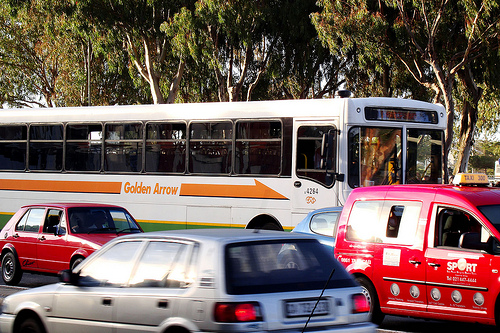
\includegraphics[width=.8\textwidth]{photos/trafficby_warrenski_flickr.jpg}\\
\textit{Foto deur warrenski op Flickr.}
\end{center}
\end{minipage}
   
\begin{enumerate}[noitemsep, label=\textbf{\arabic*}. ] 
    \item \textbf{posisie} of \textbf{verplasing} wat ons vertel van 'n voorwerp se ligging of verandering in ligging.
    \item \textbf{spoed} of \textbf{snelheid} wat vir ons vertel hoe vinnig 'n voorwerp beweeg en waarheen dit oppad is, en
    \item \textbf{versnelling} wat vir ons vertel hoe vinnig 'n voorwerp se spoed en snelheid verander. 
\end{enumerate}

\IFact{\textbf{Ruk} is die naam wat ons die verandering in versnelling noem.}

\chapterstartvideo{VPgiq}

\section{Verwysingsraamwerk}
Die eerste ding op op te fokus wanneer jy die beweging van 'n voorwerp of persoon bestudeer is hulle posisie. Die woord \textsl{posisie} beskryf jou ligging (waar jy is). Dit help egter nie om te s\^e \textsl{hier} of \textsl{daar} nie, jy moet bekende liggings (verwysingspunte) gebruik om jou posisie te spesifiseer.

\begin{minipage}{.35\textwidth}
As jy byvoorbeeld in 'n klaskamer is en jy wil vir jou klasmaats vertel waar jy staan moet jy eers vir hulle 'n verwysingspunt gee. Die verwysingspunt kan dalk die klaskamer se deur wees. Jy sal dan kan se jy is 2~m van die deur af. Dit gee nie steeds nie jou presiese posisie nie. Jy sal 'n verwysingspunt en 'n koordinaatstelsel moet defini\"eer om jou presiese ligging te kan gee.
\end{minipage}
\begin{minipage}{.6\textwidth}
\begin{center}
\textbf{Beskrywing van jou posisie}\\
 \includegraphics[width=.8\textwidth]{photos/youarehereby_chokola_flickr.jpg}\\
\textit{Foto deur chokola op Flickr.}
\end{center}
\end{minipage}\\
Jy sal dan kan s\^e jy is, byvoorbeeld, 2~m weg van die deur aan die binnekant van die klaskamer. Die klaskamer se deur is 'n verywsingspunt en binne/buite is die koordinaatstelsel wat jy gekies het. 'n Verwysingsraamwerk is die verwysingspunt wat as die oorsprong van die koordinaatstelsel dien. Die koordinaatstelsel kan op of af, binne of buite, links of regs of selfs vorentoe en aftertoe wees. Hierdie is almal voorbeelde wat 'n 1 dimensionele koordinaatstelsel defini\"eer. Ons kies een van die rigtings as die \textbf{positiewe} rigting.

\Definition{Verwysingsraamwerk} {'n Verwysingsraamwerk is die verwysings punt gekombineer met 'n stel rigtings.} 
'n Grafiese tentoonstelling van 'n 1 dimensionele verwysingsraamwerk. 
\begin{figure}[H]
 \begin{center}
  \begin{pspicture}(-2,-2)(4,4)
   \psline{->}(-1,0)(3,0)
\rput(2,0.4){$\vec{x}_{i}$}
\rput(2,0){\qdisk(0,0){3pt}}
\rput(3.3,0){$x$}
\rput(0,-1.2){oorsprong}
\psdot(0,0)
\rput[l](.2,.8){positiewe (+) rigting}
\rput[r](-.2,.8){negatiewe (--) rigting}
\psline[linestyle=dashed](0,-1)(0,1)
  \end{pspicture}
 \end{center}
\caption{verwysingsraamwerk}
\label{fig:frameofref}
\end{figure}

Jy kan verskillende verwysingsraamwerke defini\"eer vir dieselfde probleem, maar die uitslag, die fisiese resultate, sal dieselfde wees. Byvoordeeld, 'n seun staan stil in 'n trein wanneer dit uit die stasie beweeg. Jy en die seun defini\"eer julle verwysingsraamwerk as julle eie huidige posisies en die rigting waarin die trein beweeg as die vorentoe rigting. 

Jy staan op die platform en kyk hoe die trein van links na regs beweeg. Vir jou lyk dit of die seun van links na regs beweeg, want relatief tot waar jy staan (die platform), is hy besig om te beweeg. Volgens die seun, en sy verwysingsraamwerk, staan hy stil.\par 
        
'n Verwysingsraamwerk moet 'n oorsprong h\^e (waar jy staan op die platform) en ten minste 'n positiewe rigting. Die trein het van links na regs beweeg, wat na regs positief maak en na jou linkerkant toe, negatief. As iemand anders na dieselfde seun gekyk het, sou hulle verwysingsraamwerk anders gewees het. As hy, byvoorbeeld, aan die ander kant van die platform gestaan het, sou die seun van regs na links beweeg het. \par

\begin{center}
\scalebox{1.3} % Change this value to rescale the drawing.
{
\begin{pspicture}(2.5,-1.5)(12.675,2.2879686)
%\psgrid
\psline[](4.26,-2.2479687)(4.26,-2.2479687)
\psline[](4.24,-2.1679688)(4.24,-2.1679688)
\psframe[linewidth=0.04,dimen=outer](5.06,0.47203124)(3.22,0.13203125)
\psframe[linewidth=0.04,dimen=outer](7.02,0.47203124)(5.18,0.13203125)
\psframe[linewidth=0.04,dimen=outer](9.06,0.47203124)(7.22,0.13203125)
\psline[](9.22,1.4920312)(9.22,0.17203125)
\psline[](0.0,1.6920313)(0.0,1.6920313)
\psline[](9.22,1.4720312)(10.02,1.4720312)
\psline[](10.02,1.4720312)(10.02,0.77203125)
\psline[](10.02,0.77203125)(11.22,0.77203125)
\psline[](11.22,0.77203125)(11.22,0.17203125)
\psline[](11.22,0.17203125)(9.22,0.17203125)
\psline[](10.42,1.4720312)(11.02,1.4720312)
\psline[](11.02,1.4720312)(10.82,0.77203125)
\psline[](10.42,1.4720312)(10.62,0.77203125)
\pscircle[linewidth=0.04,dimen=outer](9.82,-0.12796874){0.3}
\pscircle[linewidth=0.04,dimen=outer](10.72,-0.12796874){0.3}
\pscircle[linewidth=0.04,dimen=outer](8.52,-0.12796874){0.3}
\pscircle[linewidth=0.04,dimen=outer](7.62,-0.12796874){0.3}
\pscircle[linewidth=0.04,dimen=outer](6.52,-0.12796874){0.3}
\pscircle[linewidth=0.04,dimen=outer](5.62,-0.12796874){0.3}
\pscircle[linewidth=0.04,dimen=outer](4.62,-0.12796874){0.3}
\pscircle[linewidth=0.04,dimen=outer](3.72,-0.12796874){0.3}
\psline[linewidth=0.051999997cm](5.02,0.27203125)(5.22,0.27203125)
\psline[linewidth=0.05cm](7.02,0.27203125)(7.22,0.27203125)
\psline[linewidth=0.05cm](9.22,0.27203125)(9.02,0.27203125)
\rput{-14.036243}(-0.19131365,1.5252956){\psellipse[linewidth=0.05,dimen=outer](6.099412,1.5396783)(0.15764816,0.25)}
\psline[linewidth=0.05cm](6.04,1.3120313)(6.02,0.8720313)
\psline[linewidth=0.05cm](6.02,0.8720313)(5.82,0.47203124)
\psline[linewidth=0.05cm](5.82,0.47203124)(5.92,0.47203124)
\psline[linewidth=0.05cm](6.02,0.8720313)(6.02,0.45203125)
\psline[linewidth=0.05cm](6.02,0.47203124)(6.12,0.47203124)
\psline[linewidth=0.05cm](6.04,1.1720313)(5.92,0.97203124)
\psline[linewidth=0.05cm](5.92,0.97203124)(6.12,0.8720313)
\psdots[dotsize=0.12](6.18,1.5920312)
\psline[linewidth=0.05cm,]{->}(9.2,1.8920312)(10.62,1.8920312)

\rput(10.585781,2.1120312){\scriptsize trein beweeg van links na regs}

\rput(6.494219,2.1120312){\scriptsize seun staan stil}

\rput(7.5909376,-0.9479687){\scriptsize In jou verwysingsraamwerk beweeg die seun van links na regs.}
\psline[linewidth=0.05cm](6.02,1.1720313)(6.06,0.8720313)
\psline[linewidth=0.05cm](6.06,0.9320313)(6.1,0.7920312)
\pscustom[linewidth=0.05]
{
\newpath
\moveto(6.08,1.4920312)
\lineto(6.11,1.4620312)
\curveto(6.125,1.4470313)(6.145,1.4270313)(6.16,1.4120313)
}
\pscustom[linewidth=0.05]
{
\newpath
\moveto(6.24,1.8120313)
\lineto(6.12,1.7820313)
\curveto(6.06,1.7670312)(5.99,1.7520312)(5.96,1.7520312)
}
\pscustom[linewidth=0.05]
{
\newpath
\moveto(6.14,1.8120313)
\lineto(6.11,1.8120313)
\curveto(6.095,1.8120313)(6.075,1.8120313)(6.07,1.8120313)
\curveto(6.065,1.8120313)(6.05,1.7920313)(6.04,1.7720313)
\curveto(6.03,1.7520312)(6.015,1.7270312)(6.0,1.7120312)
}
\end{pspicture}  
}
\end{center}
\begin{center}
\begin{pspicture}(0,-0.5)(5,2)
%\psgrid[gridcolor=gray]
\pcline{<->}(0.5,0.5)(4.5,0.5)
\aput{:U}{\parbox[l]{4cm}{'n Seun binne in 'n trein wat van links na regs beweeg.}}
\psline(2.5,0.6)(2.5,0.4)
\uput[d](2.5,0.4){Waar jy staan}
\uput[d](2.5,0.0){op die platform}
\uput[d](2.5,-0.4){(verwysingspunt of oorsprong)}
\uput[r](4.5,0.5){positiewe rigting (na jou regterkant)}
\uput[l](0.5,0.5){negatiewe rigting (na jou linkerkant)}
\end{pspicture}
\end{center}

In hierdie hoofstuk sal ons net verwysingsraamwerke gebruik wat in die $x$ rigting is. Sodoende beperk ons onsself tot \textsl{een dimensionele beweging}. Ons kan die teken van die posisie-waarde (positief of negatief) gebruik om die rigting relatief tot die oorsprong te wys.

\Definition{Een dimensionele beweging}{'n Voorwerp se beweging word beperk tot 'n lyn.}

Byvoorbeeld, die blou kol in die figuur kan net op die $x$ as beweeg.
 \begin{center}
  \begin{pspicture}(-2,-2)(4,4)
   \psline[linewidth=.05cm]{<->}(-3,0)(3,0)
% \rput(2,0.4){$\vec{x}_{i}$}
\rput(2,0){\pscircle[linecolor=blue,fillcolor=blue,fillstyle=solid](0,0){.2}}
\rput(3.3,0){$x$}
\rput(0,-.2){oorsprong}
\psline(0,-.1)(0,.1)
  \end{pspicture}
 \end{center}
%Frames of reference will be covered in more detail in Grade 12.\par       
	
\subsection*{Posisie}
\nopagebreak

\Definition{Posisie} {Posisie is 'n mate van ligging, met verwysing na 'n oorsprong toe.\\
Simbool: $x$\hspace{2cm} S.I. Eenheid: m} 

'n Posisie is 'n mate van 'n ligging binne 'n verwysingsraamwerk. Dit beteken dat posisie negatief of positief kan wees afhangend van die keuse van die verwysingsraamwerk se koordinaatstelsel.
\mindsetvid{Position}{VPgmf}

Afhangende van watter verwysingspunt ons kies, kan ons s\^e dat die skool $300~\text{m}$ van Kosma se huis is (met Kosma se huis as die verwysingspunt of oorsprong), of $500~\text{m}$ van Kevin se huis (met Kevin se huis as die verwysingspunt of oorsprong).\par
\begin{center}
\scalebox{1} % Change this value to rescale the drawing.
{
\begin{pspicture}(0,-1.421875)(14.005,1.386875)
\psframe[linewidth=0.05,dimen=outer](1.82,0.601875)(0.22,-0.298125)
\pstriangle[linewidth=0.05,dimen=outer](1.03,0.541875)(2.06,0.82)
\pstriangle[linewidth=0.05,dimen=outer](13.03,0.561875)(2.06,0.82)
\psline[linewidth=0.05cm,tbarsize=0.07055555cm 5.0]{|-|}(1.06,-0.918125)(13.1,-0.938125)
\psline[linewidth=0.05cm](3.08,-0.798125)(3.08,-1.038125)
\psline[linewidth=0.05cm](5.06,-0.798125)(5.06,-1.038125)
\psline[linewidth=0.05cm](7.06,-0.818125)(7.06,-1.038125)
\psline[linewidth=0.05cm](9.06,-0.798125)(9.06,-1.038125)
\psline[linewidth=0.05cm](11.06,-0.778125)(11.06,-1.018125)

\rput(2.085,-1.283125){\footnotesize $100 ~\text{m}$}
\psframe[linewidth=0.05,dimen=outer](13.86,0.621875)(12.26,-0.278125)
\psframe[linewidth=0.05,dimen=outer](3.62,0.581875)(2.54,-0.298125)
\psframe[linewidth=0.05,dimen=outer](5.6,0.581875)(4.52,-0.298125)
\psframe[linewidth=0.05,dimen=outer](7.6,0.581875)(6.52,-0.298125)
\psframe[linewidth=0.05,dimen=outer](9.62,0.581875)(8.54,-0.298125)
\psframe[linewidth=0.05,dimen=outer](11.62,0.581875)(10.54,-0.298125)
\pstriangle[linewidth=0.05,dimen=outer](3.08,0.521875)(1.36,0.54)
\pstriangle[linewidth=0.05,dimen=outer](7.06,0.521875)(1.36,0.54)
\pstriangle[linewidth=0.05,dimen=outer](5.04,0.521875)(1.36,0.54)
\pstriangle[linewidth=0.05,dimen=outer](9.06,0.521875)(1.36,0.54)
\pstriangle[linewidth=0.05,dimen=outer](11.08,0.521875)(1.36,0.54)

\rput(4.105,-1.263125){\footnotesize $100 ~\text{m}$}

\rput(6.105,-1.283125){\footnotesize $100 ~\text{m}$}

\rput(8.125,-1.263125){\footnotesize $100 ~\text{m}$}

\rput(10.125,-1.263125){\footnotesize $100 ~\text{m}$}

\rput(12.125,-1.283125){\footnotesize $100 ~\text{m}$}

\rput(13.068594,0.161875){\small Winkel}

\rput(1.065,0.171875){Skool}

\rput(3.0773437,0.171875){\small{Komal}}

\rput(5.0554686,0.171875){\small{Kholo}}

\rput(7.065469,0.171875){\small{Kosma}}

\rput(9.0725,0.171875){\small{Kogis}}

\rput(11.065469,0.171875){\small{Kevin}}
\end{pspicture} 
}
\end{center}

Die winkel is ook $300~m$ can Kosma se huis af, maar in die teenoorgestelde rigting as die skool. Wanneer ons 'n verwysingspunt kies, het ons 'n positiewe en negatiewe rigting. As ons die rigting na die skool toe as negatief kies, dan is die rigting na die winkel toe positief. 'n Negatiewe rigting is altyd in die teenoorgestelde rigting as die rigting wat as positief gekies is. 
    
\begin{center}
\scalebox{1} % Change this value to rescale the drawing.
{
\begin{pspicture}(0,-1.1871876)(9.225,1.1871876)
\psline[linewidth=0.05cm,]{<->}(0.0,-0.6428125)(8.0,-0.6428125)
\psline[linewidth=0.05cm](1.02,-0.5028125)(1.02,-0.7828125)
\psline[linewidth=0.05cm](2.02,-0.5028125)(2.02,-0.7828125)
\psline[linewidth=0.05cm](3.0,-0.5028125)(3.0,-0.7828125)
\psline[linewidth=0.05cm](4.02,-0.5028125)(4.02,-0.7828125)
\psline[linewidth=0.05cm](5.02,-0.5028125)(5.02,-0.7828125)
\psline[linewidth=0.05cm](6.02,-0.5028125)(6.02,-0.7828125)
\psline[linewidth=0.05cm](7.02,-0.5028125)(7.02,-0.7828125)

\rput(0.97625,-1.0328125){$-300$}

\rput(1.97625,-1.0328125){$-200$}

\rput(2.97625,-1.0328125){$-100$}

\rput(3.9970312,-1.0128125){$0$}

\rput(5.0025,-1.0128125){$+100$}

\rput(6.0196877,-1.0128125){$+200$}

\rput(7.01625,-1.0128125){$+300$}
\psline[linewidth=0.05cm,]{->}(1.0,0.2971875)(1.0,-0.4428125)
\psline[linewidth=0.05cm,]{->}(4.02,0.3171875)(4.02,-0.4628125)
\psline[linewidth=0.05cm,]{->}(7.02,0.2971875)(7.02,-0.4828125)

\rput(0.965,0.6871875){Skool}

\rput(4.101094,1.0071875){Kosma se huis}

\rput(4.1451564,0.6071875){(verwysingspunt)}

\rput(7.012656,0.6871875){Winkel}

\rput(8.612968,-0.5928125){$x$ (m)}
\end{pspicture}  }
\end{center}

Die oorsprong is by Kosma se huis en die posisie van die skool is $-300~\text{m}$. Posisies na links word gedefini\"eer as negatief en posisies na regs as positief.

Neem kennis dat ons ook die rigting na die skool as positief kan kies. In hierdie geval is Kosma se huis nog steeds $300~m$ van die skool af, maar dit is nou in die positiewe rigting.

\begin{center}
\scalebox{1} % Change this value to rescale the drawing.
{
\begin{pspicture}(0,-1.1871876)(9.225,1.1871876)
\psline[linewidth=0.05cm,]{<->}(0.0,-0.6428125)(8.0,-0.6428125)
\psline[linewidth=0.05cm](1.02,-0.5028125)(1.02,-0.7828125)
\psline[linewidth=0.05cm](2.02,-0.5028125)(2.02,-0.7828125)
\psline[linewidth=0.05cm](3.0,-0.5028125)(3.0,-0.7828125)
\psline[linewidth=0.05cm](4.02,-0.5028125)(4.02,-0.7828125)
\psline[linewidth=0.05cm](5.02,-0.5028125)(5.02,-0.7828125)
\psline[linewidth=0.05cm](6.02,-0.5028125)(6.02,-0.7828125)
\psline[linewidth=0.05cm](7.02,-0.5028125)(7.02,-0.7828125)

\rput(0.97625,-1.0328125){$+300$}

\rput(1.97625,-1.0328125){$+200$}

\rput(2.97625,-1.0328125){$+100$}

\rput(3.9970312,-1.0128125){$0$}

\rput(5.0025,-1.0128125){$-100$}

\rput(6.0196877,-1.0128125){$-200$}

\rput(7.01625,-1.0128125){$-300$}
\psline[linewidth=0.05cm,]{->}(1.0,0.2971875)(1.0,-0.4428125)
\psline[linewidth=0.05cm,]{->}(4.02,0.3171875)(4.02,-0.4628125)
\psline[linewidth=0.05cm,]{->}(7.02,0.2971875)(7.02,-0.4828125)

\rput(0.965,0.6871875){Skool}

\rput(4.101094,1.0071875){Kosma se huis}

\rput(4.1451564,0.6071875){(verwysingspunt)}

\rput(7.012656,0.6871875){Winkel}

\rput(8.612968,-0.5928125){$x$ (m)}
\end{pspicture}  }

\end{center}

Die oorsprong is by Kosma se huis en die posisie van die skool is $+300~\text{m}$. Posisies na links word as positief gedefini\"eer en posisies na regs as negatief.

\begin{groupdiscussion}{Verwysingspunte}
            \nopagebreak
Deel op in groepe van 5 vir hierdie aktiwiteit. Kies 'n verwysingspunt vir 'n reguit lyn. Omdat posisie beide negatiewe en positiewe waardes kan h\^e, bespreek die voor- en nadele as jy die verwysingspunt kies as:
\begin{enumerate}[noitemsep, label=\textbf{\arabic*}. ] 
    \item een kant van die lyn
    \item die middel van die lyn. (Hierdie verwysingspunt kan ook die ``oorsprong'' genoem word.)
\end{enumerate}
Staan in 'n reguit lyn, maak beurte om verskillende mense in jou groep te kies as die oorsprong. Laat die persoon wat die oorsprong is toe om die positiewe rigting te kies. Elkeen behoort dan te probeer om hulle posisies te defini\"eer. Die posisies hoef nie baie presies te wees nie maar jy kan 'n benadering maak. Dit is belangrik om te verstaan hoekom jou posisie positief of negatief is vir elke verskillende oorsprong en koordinaatstelsel.

Neem kennis dat jou posisie elke keer verskillend is maar dat jy nie beweeg het nie. Die manier hoe 'n antwoord geskryf word kan deur die koordinaatstelsel be\"invloed word maar fisiese prosesse behoort nooit be\"invloed te word nie.
\end{groupdiscussion}

\begin{exercises}{Posisie}
\begin{enumerate}[noitemsep, label=\textbf{\arabic*}. ] 
    \item Skryf die posisies neer van voorwerpe by A, B, D en E. Moenie die eenhede vergeet nie.
\begin{figure}[H] % horizontal\label{m38787*id62877}
\begin{center}
\begin{pspicture*}(-6,-1)(6.1,1)
\psset{dotsize=7pt}
%\psgrid[gridcolor=lightgray]
\multirput(0,0)(0,0){1}{
\multido{\n=-4+1}{9}
{\psline{<->}(-5,0)(5,0)
\rput(\n,0){\psline(0,-0.1)(0,0.1)}
\uput[d](\n,-0.1){\n}}
\uput[r](5,0){$x$ (m)}}
\uput[u](0,0.5){verwysingspunt}
\uput[u](-3,0.2){A}
\uput[u](-1,0.2){B}
\uput[u](1,0.2){D}
\uput[u](3,0.2){E}
\psline{->}(0,0.6)(0,0.2)
\end{pspicture*}
\end{center}
 \end{figure}

\item Skryf die posisies neer van voorwerpe by F,G,H en J. Moenie die eenhede vergeet nie.
\begin{figure}[H] % horizontal\label{m38787*id62899}
\begin{center}
\begin{pspicture*}(-6,-1)(6.1,1)
\psset{dotsize=7pt}
%\psgrid[gridcolor=lightgray]
\multirput(0,0)(0,0){1}{
\multido{\n=-4+1}{9}
{\psline{<->}(-5,0)(5,0)
\rput(\n,0){\psline(0,-0.1)(0,0.1)}
\uput[d](-\n,-0.1){\n}}
\uput[r](5,0){$x$ (m)}}
\uput[u](0,0.5){verwysingspunt}
\uput[u](-3,0.2){F}
\uput[u](-1,0.2){G}
\uput[u](1,0.2){H}
\uput[u](3,0.2){J}
\psline{->}(0,0.6)(0,0.2)
\end{pspicture*}
\end{center}
 \end{figure}

\item Daar is 5 huise op Newton straat, A, B, C, D en E. Neem aan die posisies na regs is positief.
\begin{figure}[H] % horizontal\label{m38787*id62920}
\begin{center}
\begin{pspicture*}(-4.2,-0.2)(5.2,2.8)
\def\house{\psframe(0,0)(1,1)\pspolygon(0,1)(0.5,2)(1,1)}
\def\distance{\psline(0.5,2.2)(0.5,2.4)\psline(2.5,2.2)(2.5,2.4)\psline{<->}(0.5,2.3)(2.5,2.3)\uput[u](1.5,2.3){20 m}}
\psset{dotsize=7pt}
%\psgrid[gridcolor=lightgray]
\multirput(-4,0)(2,0){5}{\house}
\multirput(-4,0)(2,0){4}{\distance}
\rput(-3.5,0.5){\Large{\textsf{A}}}
\rput(-1.5,0.5){\Large{\textsf{B}}}
\rput(0.5,0.5){\Large{\textsf{C}}}
\rput(2.5,0.5){\Large{\textsf{D}}}
\rput(4.5,0.5){\Large{\textsf{E}}}
\end{pspicture*}
\end{center}
 \end{figure}       

 
\begin{enumerate}[noitemsep, label=\textbf{\alph*}. ] 
    \item Teken 'n verwysingsraamwerk met huis A as oorsprong en skryf dan die posisies neer van huise B, C, D en E.
    \item Jy bly in huis C. Wat is jou posisie relatief tot huis E?
    \item Wat is die posisies van huise A, B en D as huis B as die verwysingspunt gekies word?
\end{enumerate}
\end{enumerate}

\practiceinfo
 \par \begin{tabular}[h]{cccccc}
 (1.) laG  &  (2.) la7  &  (3.) laA  & \end{tabular}
\end{exercises}

\Tip{Die simbool $\Delta $ word gelees as \textsl{delta}. $\Delta $ is 'n letter van die Griekse alfabet en word in Wiskunde en Wetenskap gebruik om 'n verandering van 'n hoeveelheid, of finale waarde minus aanvanklike waarde, aan te dui. Byvoorbeeld, $\Delta x$ beteken verandering in $x$ terwyl $\Delta t$ verandering in $t$ aandui.}
\subsection*{Verplasing en afstand}
    \nopagebreak
%            \label{m38788} $ \hspace{-5pt}\begin{array}{cccccccccccc}   \end{array} $ \hspace{2 pt}\raisebox{-0.2em}{
\includegraphics[height=1em]{../icons/www.pdf}} {(section shortcode: P10098 )} \par 
\Definition{Verplasing}{ Verplasing is die verandering in 'n voorwerp se posisie. Dit is 'n vektor van die oorspronklike posisie ($\vec{x}_{i}$) na die finale posisie ($\vec{x}_{f}$) wys.\par
Simbool: $\Delta \vec{x}$\hspace{2cm} S.I. Eenheid: $\text{m}$ }

Die verplasing van 'n voorwerp word gedefini\"eer as die verandering in posisie (finale posisie minus aanvanklike posisie). Verplasing het 'n grootte en 'n rigting en is dus 'n vektor. Byvoorbeeld, as die aanvanklike posisie van 'n kar $\vec{x}_{i}$ is en dit beweeg na 'n finale posisie $\vec{x}_{f}$, dan is die verplasing:

        
\begin{equation*}
    \vec{x}_{f}-\vec{x}_{i}
  \end{equation*}
Dit help om die verplasing te visualiseer as jy terug dink aan die stert-na-kop metode. Die verplasing is die vektor wat jy by die aanvanklike posisie tel om die finale posisie te kry.

In Fisika gebruik ons egter die kortpad $\Delta$ om aan te dui dat ons 'n aanvanklike posisie van 'n finale een afgetrek het,     dus skryf ons: 
\begin{equation*}
    \Delta \vec{x}=\vec{x}_{f}-\vec{x}_{i}
\end{equation*}


Die volgende diagram illustreer die konsep van verplasing:
\begin{figure}[H]
 \begin{center}
  \begin{pspicture}(-2,-2)(5,5)
   \psline{<->}(-1,0)(4,0)
\rput(1,0){\qdisk(0,0){2pt}}
\rput(3,0){\qdisk(0,0){2pt}}
\rput[t](0,0.5){$0$}
\psline(0,-.2)(0,.2)
\rput[t](1,0.5){$\vec{x}_{i}$}
\rput[t](3,0.5){$\vec{x}_{f}$}
\psline{->}(1,-.3)(3,-0.3)
\rput[b](2,-.7){$\Delta \vec{x}$}
  \end{pspicture}
 \end{center}
\end{figure}
As jy byvoorbeeld 'n bal $5~\text{m}$ ver in 'n reguit lyn rol is sy verplasing $5~\text{m}$, indien jy die rigting waarin die bal rol as positief vat en die aanvanklike posisie as $0~\text{m}$.

\Tip{Die woorde \textsl{aanvanklik} end \textsl{finaal} word dikwels in Fisika gebruik. \textsl{Aanvanklik} verwys na die situasie aan die begin van die beskrywing/probleem en \textsl{finaal} na die situasie aan die einde. Dit gebeur ook dikwels dat die finale waarde kleiner as die aanvanklike waarde is wat maak dat die verskil negatief is. Dit is nie 'n probleem nie!}
     
Verplasing is nie afhanklik van die pad wat gevolg word nie, net die aanvaklike en finale posisies. Ons gebruik die woord \textsl{afstand} as ons wil beskryf hoe ver 'n voorwerp op 'n sekere pad beweeg het.

\Tip{Ons sal $D$ in hierdie boek gebruik, maar jy sal dalk $d$ in ander boeke sien.}

\Definition{Afstand}{Afstand is die totale lengte van die pad wat gevolg word van die aanvanklike posisie, $\vec{x}_{i}$, na die finale posisie, $\vec{x}_{f}$. Afstand is 'n skalaar.\\Simbool: $D$\hspace{2cm} S.I. Eenheid: $\text{m}$}

In die diagram hieronder kan jy sien dat die pad kronkel as gevolg van heuwels vanaf 'n skool na 'n nabye winkel. Die pad word as 'n strepieslyn aangedui. \\

\begin{minipage}{.5\textwidth}
Afstand is die lengte van die strepieslyn. Dit is hoe very jy sal moet stap as jy die pad volg. Die verplasing is anders. Verplasing is die reguit lyn van die beginpunt tot by die eindpuny -- van die skool na die winkel soos aangedui met die pyl in die figuur.
\end{minipage}
\begin{minipage}{.5\textwidth}
\begin{center}
\begin{pspicture}(0.2,0.2)(5,5)
%\psgrid[gridcolor=lightgray]
\psdots(0.5,1)\psdots(4.5,1)
\pscurve[linestyle=dashed,linecolor=blue](0.5,1)(1,1.5)(2,2.5)(2.5,0)(4,2)(4.5,1)
\rput(0.5,0.7){Begin}
\rput(0.5,0.3){(Skool)}
\rput(4.5,0.7){Einde}
\rput(4.5,0.3){(Winkel)}
% \psline[linewidth=0.05, linestyle=dotted, arrowscale=2]{->}(0.5,1)(4.4,1)
% \psline[linewidth=0.05, linestyle=dotted,arrowscale=2]{->}(4.4,1)(4.4,4.4)
\pcline[arrowscale=2]{->}(0.5,1)(4.5,1)
% \lput*{:U}{Displacement}
\end{pspicture}
\end{center}
\end{minipage}
\Tip{Ons gebruik die uitdrukking \textsl{'soos die kraai vlieg'} om 'n reguit lyn tussen twee punte te beskryf, omdat vo\"els reguit oor hindernisse kan vlieg.}

\mindsetvid{Distance and displacement}{VPgmo}
\subsubsection*{Illustrasie van verplasing en afstand}
As ons dieselfde situasie as vantevore gebruik kan ons die konsep in meer detail bestudeer. Beskou ons beskrywing van die ligging van die huise, die skool en die winkel.

\begin{figure}
\centering
\scalebox{1} % Change this value to rescale the drawing.
{
\begin{pspicture}(0,-1.421875)(14.005,1.386875)
\psframe[linewidth=0.05,dimen=outer](1.82,0.601875)(0.22,-0.298125)
\pstriangle[linewidth=0.05,dimen=outer](1.03,0.541875)(2.06,0.82)
\pstriangle[linewidth=0.05,dimen=outer](13.03,0.561875)(2.06,0.82)
\psline[linewidth=0.05cm,tbarsize=0.07055555cm 5.0]{|-|}(1.06,-0.918125)(13.1,-0.938125)
\psline[linewidth=0.05cm](3.08,-0.798125)(3.08,-1.038125)
\psline[linewidth=0.05cm](5.06,-0.798125)(5.06,-1.038125)
\psline[linewidth=0.05cm](7.06,-0.818125)(7.06,-1.038125)
\psline[linewidth=0.05cm](9.06,-0.798125)(9.06,-1.038125)
\psline[linewidth=0.05cm](11.06,-0.778125)(11.06,-1.018125)

\rput(2.085,-1.283125){\footnotesize $100 ~\text{m}$}
\psframe[linewidth=0.05,dimen=outer](13.86,0.621875)(12.26,-0.278125)
\psframe[linewidth=0.05,dimen=outer](3.62,0.581875)(2.54,-0.298125)
\psframe[linewidth=0.05,dimen=outer](5.6,0.581875)(4.52,-0.298125)
\psframe[linewidth=0.05,dimen=outer](7.6,0.581875)(6.52,-0.298125)
\psframe[linewidth=0.05,dimen=outer](9.62,0.581875)(8.54,-0.298125)
\psframe[linewidth=0.05,dimen=outer](11.62,0.581875)(10.54,-0.298125)
\pstriangle[linewidth=0.05,dimen=outer](3.08,0.521875)(1.36,0.54)
\pstriangle[linewidth=0.05,dimen=outer](7.06,0.521875)(1.36,0.54)
\pstriangle[linewidth=0.05,dimen=outer](5.04,0.521875)(1.36,0.54)
\pstriangle[linewidth=0.05,dimen=outer](9.06,0.521875)(1.36,0.54)
\pstriangle[linewidth=0.05,dimen=outer](11.08,0.521875)(1.36,0.54)

\rput(4.105,-1.263125){\footnotesize $100 ~\text{m}$}

\rput(6.105,-1.283125){\footnotesize $100 ~\text{m}$}

\rput(8.125,-1.263125){\footnotesize $100 ~\text{m}$}

\rput(10.125,-1.263125){\footnotesize $100 ~\text{m}$}

\rput(12.125,-1.283125){\footnotesize $100 ~\text{m}$}

\rput(13.068594,0.161875){\small Winkel}

\rput(1.065,0.171875){Skool}

\rput(3.0773437,0.171875){\small{Komal}}

\rput(5.0554686,0.171875){\small{Kholo}}

\rput(7.065469,0.171875){\small{Kosma}}

\rput(9.0725,0.171875){\small{Kogis}}

\rput(11.065469,0.171875){\small{Kevin}}
\end{pspicture} 
}
\caption{}
\label{position:reference3}
\end{figure}
Komal stap om vir Kevin by sy huis te ontmoet voor hulle skool toe stap. Wat is Komal se verplasing en wat is die afstand wat hy moet stap as hy skool toe stap via Kevin se huis?

Komal l\^e 'n afstand van $400~m$ af na Kevin se huis toe en nog $500~m$ van Kevin se huis na die skool. Hy l\^e dus 'n totale afstand van $900~m$ af. Sy verplasing is egter net $100~m$ na die skool toe. Die rede is omdat verplasing net die beginpunt (sy huis) en die eindpunt (die skool) in ag neem. Dit is nie afhanklik van die roete wat hy geneem het nie.

Om die afstand en verplasing te bereken moet ons 'n verwysingspunt en 'n rigting kies. Kom ons kies Komal se huis as die verwysingspunt en die rigting na Kevin se huis as die positiewe rigting (dit beteken die rigting na die skool toe is negatief). Ons doen die berekeninge dan as volg:\par 
\begin{minipage}{0.35\textwidth}
\begin{eqnarray*}
\text{Afstand (D)} &=& \text{roete gevolg}\\
&=&400\ \text{m} + 500\ \text{m}\\
&=&900\ \text{m}\\
\end{eqnarray*}
\end{minipage}
\begin{minipage}{0.65\textwidth}
\begin{eqnarray*}
\text{Verplasing} (\Delta \vec{x}) &=& \vec{x}_f~ - ~ \vec{x}_i\\
&=&-100\ \text{m} + 0\ \text{m}\\
&=&-100\ \text{m}\\
&=&100\ \text{m} \text{( in ~die~ negatiewe~} x \text{~rigting)}
\end{eqnarray*}
\end{minipage}\par


Jy sal gereeld negatiewe antwoorde in jou berekeninge kry. Byvoorbeeld, Komal se verplasing in die voorbeeld hierbo is as $-100~m$ bereken. Die minus teken voor die antwoord wys dat sy verplasing $100~m$ in die teenoorgestelde rigting (teenoorgestelde rigting as die rigting wat as positief gekies is) is. Wanneer ons 'n berekening begin, kies ons 'n verwysingsraamwerk en 'n positiewe rigting. In die eerste voorbeeld hierbo was dit verwysingspunt Komal se huis en die positiewe rigting was na Kevin se huis toe. Komal se verplasing is dus $100~m$ na die skool toe. Neem kennis dat afstand nie 'n rigting het nie maar verplasing het wel.\par


Kevin stap skool toe saam met Komal en na skool loop hy terug huis toe. Wat is Kevin se verplasing en watter afstand het hy afgel\^e? Vir hierdie berekening gebruik ons Kevin se huis as die verwysingspunt. Kom ons neem aan die rigting na die skool toe is positief.\\
\begin{minipage}{0.5\textwidth}
\begin{eqnarray*}
\text{Afstand (D)} &=& \text{roete~gevolg}\\
&=&500\ \text{m} + 500\ \text{m}\\
&=&1000\ \text{m}
\end{eqnarray*}
\end{minipage}
\begin{minipage}{0.5\textwidth}
\begin{eqnarray*}
\text{Verplasing} (\Delta \vec{x}) &=& \vec{x}_f~ - ~ \vec{x}_i\\
&=&0\ \text{m} + 0\ \text{m}\\
&=&0\ \text{m}
\end{eqnarray*}
\end{minipage} 
\par
Dit is moontlik om 'n verplasing van $0~m$ te h\^e en 'n afstand wat nie $0~m$ is nie. Dit gebeur wanneer jy eindig waar jy begin het.

\subsubsection*{Die verskil tussen afstand en verplasing}
            \nopagebreak
Die verskille tussen afstand en verplasing kan as volg opgesom word:\par
\begin{center}
\begin{tabular}{|l|l|}\hline
\textbf{ Afstand} & \textbf{ Verplasing} \\\hline
1. Afhanklik van roete & 1. Onafhanklik van roete \\\hline
2. altyd positief & 2. negatief of positief \\\hline
3. is 'n skalaar & 3. is 'n vektor\\\hline
\end{tabular}
\end{center}
    \par
\label{m38788*secfhsst!!!underscore!!!id498}
\begin{exercises}{Verwysingsraamwerke, verplasing en afstand}
\nopagebreak \noindent
\begin{enumerate}[noitemsep, label=\textbf{\arabic*}. ] 
\item Gebruik Figuur~\ref{position:reference3} om die volgende te beantwoord.
\begin{enumerate}[noitemsep, label=\textbf{\alph*}. ] 
    \item Kogis stap na Kosma se huis en dan skool toe. Wat is haar afstand en verplasing?
    \item Kholo stap na Kosma se huis en dan skool toe. Wat is haar afstand en verplasing?
    \item Komal stap winkel en daarna skool toe.i Wat is sy afstand en verplasing?
    \item Watter verwysingspunt het jy vir elk van die vrae gebruik?
\end{enumerate}
                
\item Jy staan by die voordeur van jou huis (verplasing, $\Delta \vec{x}=0~\text{m}$). Die straat is $10~\text{m}$ van die voordeur af. Jy stap na die straat toe en terug.
\begin{enumerate}[noitemsep, label=\textbf{\alph*}. ] 
    \item Wat is die afstand wat jy gestap het?
    \item Wat is jou finale verplasing?
    \item Is verplasing 'n vektor of 'n skalaar? Gee redes vir jou antwoord.
\end{enumerate}
\end{enumerate}
  \label{m38788**end}
\practiceinfo
 \par \begin{tabular}[h]{cccccc}
 (1.) lDl  &  (2.) las  & \end{tabular}
\end{exercises}



\section{Spoed and snelheid} 
    \nopagebreak

\Definition{Gemiddelde spoed}
{Gemiddelde spoed is die \textbf{afstand} ($D$) afgel\^e gedeel deur die tyd ($\Delta t$) wat die reis geneem het.\\
Simbool: $v_{av}$\hspace{2cm} S.I. Eenhede: $\text{m}\cdot \text{s}^{-1}$} 


\Definition{Gemiddelde snelheid}{Gemiddelde snelheid is die \textbf{verplasing} van 'n liggam gedeel deur die tyd wat dit geneem het vir die verplasing om te gebeur.\\
Simbool: $\vec{v}_{av}$\hspace{2cm} S.I. Eenhede: $\text{m}\cdot \text{s}^{-1}$} 

Neem kennis dat die gemiddelde spoed 'n groot waarde kan h\^e terwyl die gemiddelde snelheid nul is. \mindsetvid{VPgjq}


Gemiddelde snelheid is die tempo waarteen posisie verander. Dit s\^e vir ons hoeveel 'n voorwerp se se posisie verander in 'n eenheid van tyd. Snelheid is 'n vektor. Ons gebruik die simbool $\vec{v}_{av}$ vir gemiddelde snelheid. As ons 'n verplasing het van $\Delta \vec{x}$ en 'n tyd geneem van $\Delta t$ word $\vec{v}_{av}$ dan gedefini\"eer as:\par 
\begin{eqnarray*}
\text{gemiddelde snelheid (in m} \cdot \text{s}^{-1}) &=& \frac{\text{verandering in verplasing (in m)}}{\text{verandering in tyd (in s)}}\\
\vec{v}_{av} &=& \frac{\Delta \vec{x}}{\Delta t}
\end{eqnarray*}\label{eq:pr:velocity}
Snelheid kan positief of negatief wees. 'n Positiewe snelheid wys in die rigting wat jy as positief gekies het in jou koordinaatstelsel. 'n Negatiewe snelheid wys in die teenoorgestelde rigting as die positiewe rigting.

Gemiddelde spoed (simbool $v_{av}$) is die afstand wat afgel\^e is ($D$), gedeel deur die tyd ($\Delta t$) wat dit geneem het om die afstand af te \^e. Afstand en tyd is skalare en dus is spoed ook 'n skalaar. Spoed word as volg bereken:\par 
        
\begin{equation*}
\text{gemiddelde spoed (in m} \cdot {\text{s}}^{-1}\text{)}  =  \frac{\text{afstand (in m)}}{\text{tyd (in s)}} 
\end{equation*}
\label{m38791*id64639}\nopagebreak\noindent{}
\begin{equation*}
v_{av}=\frac{D}{\Delta t}
\end{equation*}
     

 
\begin{wex}{Gemiddelde spoed en snelheid}
{James stap $2 \text{ km}$ van sy huis af in 30 minute. Hy draai dan om en stap huis toe volgens dieselfde roete, ook in 30 minute. Bereken James se gemiddelde spoed en gemiddelde snelheid.\\
\begin{center}
\begin{pspicture}(0,0)(3,0.5)
%\psgrid
\psline[linewidth=1pt]{->}(0,0)(2,0)
\psline[linewidth=1pt]{->}(2,0.5)(0,0.5)
% \psarc[linewidth=1pt]{->}(2.1,0.25){0.25}{-90}{90}
\uput[d](1,1){$2 \text{ km}$}
\end{pspicture}
\end{center}}
{

\westep{Identifiseer watter inligting gegee is en wat verlang word.}
Die vraag gee uitdruklik
\begin{itemize}
    \item die afstand en tyd daarheen ($2\text{ km}$ in 30 minute)
    \item die afstand en tyd terug ($2\text{ km}$ in 30 minute)
\end{itemize}

\westep{Maak seker dat alle eenhede SI eenhede is}
Die informasie is nie in SI eenhede nie en moet dus omgeskakel word.\\
Om km na m om te skakel weet ons dat:
\begin{eqnarray*}
1\ \text{km} &=&1\ 000\ \text{m}\\
\therefore\quad 2\ \text{km} &=&2\ 000\ \text{m} \quad \text{(vermenigvuldig albei kante met $2$.)}
\end{eqnarray*}
Op 'n soortgelyke manier kan ons 30 minute na sekondes omskakel
\begin{eqnarray*}
1\ \text{min} &=&60 \text{s}\\
\therefore\quad 30\ \text{min} &=&1\ 800\ \text{s} \quad \mbox{(vermenigvuldig albei kante met 30)}
\end{eqnarray*}

\westep{Bereken James se verplasing en afstand}
James het by die huis begin en teruggekeer huis toe, sy verplasing is dus 0 m.
$\Delta \vec{x} = 0\ \text{m}$\\
James het 'n totale afstand van $4 000 \text{ m}$ ($2\ 000\text{ m}$ daarheen en $2\ 000\text{ m}$ terug).\\
$D = 4\ 000\;\text{m}$
 
\westep{Bereken sy totale tyd}
James het $1~800\text{ s}$ geneem om daarheen te stap en $1~800\text{ s}$ om terug te stap.\\
$\Delta t = 3\ 600\;\text{s}$

\westep{Bereken sy gemiddelde spoed}
\begin{eqnarray*}
v_{av}&=&\frac{D}{\Delta t}\\
&=&\frac{4\ 000\ \text{m}}{3\ 600\ \text{s}}\\
&=&1,11\ ~\text{m}\cdot \text{s}^{-1}
\end{eqnarray*}

\westep{Bereken sy gemiddelde snelheid}
\begin{eqnarray*}
{\vec{v}_{av}}&=&\frac{\Delta \vec{x}}{\Delta t}\\
&=&\frac{0\ \text{m}}{3\ 600\ \text{s}}\\
&=& 0\ ~\text{m}\cdot \text{s}^{-1}
\end{eqnarray*}}
\end{wex}


\subsection*{Die verskil tussen sped en snelheid}
Die verskille tussen spoed en snelheid kan as volg opgesom word:\par
\begin{center}
\begin{tabular}{|p{5cm}|p{5cm}|}\hline
\textbf{Spoed} & \textbf{Snelheid} \\\hline
1. afhanklik van die roete & 1. onafhanklik van die roete \\\hline
2. altyd positief & 2. kan positief of negatief wees \\\hline
3. is 'n skalaar & 3. is 'n vektor \\\hline
4. onafhanklik van rigting en is dus positief & 4. rigting kan bepaal word van die teken (d.w.s. positief of negatief) \\\hline
\end{tabular}
\end{center}
    \par
Daarbenewens kan 'n voorwerp 'n op 'n plek begin en terugkeer na dieselfde plek en 'n snelheid van 0 h\^e maar 'n teen 'n nie-nul spoed beweeg. \par

\begin{exercises}{Verplasing en verwante hoeveelhede} \noindent
\nopagebreak
\begin{enumerate}[noitemsep, label=\textbf{\arabic*}. ] 
    \item Bongani moet winkel toe stap om melk te koop. Nadat hy $100~\text{m}$ gestap het kom hy agter hy het nie genoeg geld gebring nie en stap terug huis toe. As dit hom twee minute geneem het om die huis te verlaat en terug te keer, bereken die volgende:
    \begin{enumerate}[noitemsep, label=\textbf{\alph*}. ] 
        \item Hoe lank wys hy buite die huis (die tydsinterval $\Delta t$ in sekondes)?
        \item Hoe ver het hy gestap (afstand ($D$))?
        \item Wat was sy verplasing ($\Delta \vec{x}$)?
        \item Wat was sy gemiddelde snelheid (in $\text{m} \cdot \text{s}^{-1}$)?
        \item Wat was sy gemiddelde spoed (in $\text{m} \cdot \text{s}^{-1}$)?
\end{enumerate}
	
\begin{figure}[H] % horizontal\label{m38791*id66785}
\begin{center}
\scalebox{0.5} % Change this value to rescale the drawing.
{
\begin{pspicture}(0,-3.7525)(6.5721874,3.7325)
\psline[]{->}(5.4625,-2.4475)(-5.8225,-2.4675)
\psline[]{->}(-5.8825,-2.7875)(5.4625,-2.7875)
\rput(0,-3.1575){\huge 100 m}
\rput(0,-1.3){\huge 2 minute daarheen en terug}
\rput(0,-2){\huge $100 \text{ m}$}
\rput(6.53625,-2.5975){\huge huis}
\rput(-6.70765626,-2.5975){\huge winkel}
\end{pspicture} 
}
\end{center}
\end{figure}

\item Bridget kyk na 'n reguit stuk pad vanuit haar klaskamer se venster. Sy kan twee pale sien wat sy vroe\"er gemeet het as $50\text{ m}$ van mekaar af. Sy gebruik haar stophorlosie om te meet dat meeste karre $3 \text{ s}$ neem om van een paal na die volgende te ry.
\begin{enumerate}[noitemsep, label=\textbf{\alph*}. ] 
    \item Gebruik die vergelyking vir snelheid, ($\vec{v}_{av}$ = $\frac{\Delta \vec{x}}{\Delta t}$), en wys al die stappe wat nodig is om die snelheid van 'n kar te bereken wat van links na regs beweeg.
    \item As Bridget die snelheid van 'n rooi Golf meet as $-16,67~\text{m}\ensuremath{\cdot}\text{s}{}^{-1}$, in watter rigting beweeg die Golf?\par
    Bridget los haar stophorlosie aan en sien dat 'n taxi by $t=5,0~\text{s}$ verby die linkerkantste paal ry en 'n bus wat terselfdertyd verby die regterkantste paal ry. By die tyd $t=7,5~\text{s}$ ry die taxi verby die regterkantste paal. Wanneer die tyd $t=9,0~\text{s}$ is, ry die bus verby die linkerkantste paal.
    \item Hoe lank het dit die taxi en die bus geneem om tussen die twee pale te ry? (Bereken die tydsinterval ($\Delta t$) vir beide die taxi en die bus).
    \item Wat was die gemiddelde snelheid van die taxi en die bus?
    \item Wat was die gemiddelde spoed van die taxi en die bus?
    \item Wat was die gemiddelde spoed van die taxi en die bus in $\text{km}\ensuremath{\cdot}\text{h}{}^{-1}$?
\end{enumerate}
	\begin{figure}[H] % horizontal\label{m38791*id66998}
\begin{center}
\scalebox{1} % Change this value to rescale the drawing.
{
\begin{pspicture}(0,-3.22)(6.74,3.2)
\psframe[linewidth=0.04,dimen=outer](1.12,3.2)(1.02,0.2)
\psframe[linewidth=0.04,dimen=outer](5.22,3.2)(5.12,0.2)
\psline[]{<->}(1.12,0.3)(5.12,0.3)

\rput(3.080625,0.61){50 m}
\psline[](0.82,-0.4)(1.12,-0.5)
\psline[](1.12,-0.5)(1.12,-0.7)
\psline[](1.12,-0.7)(0.92,-0.7)
\psline[](0.72,-0.7)(0.42,-0.7)
\psline[](0.72,-0.2)(0.82,-0.4)
\pscircle[linewidth=0.04,dimen=outer](0.32,-0.7){0.1}
\pscircle[linewidth=0.04,dimen=outer](0.82,-0.7){0.1}
\psline[](0.72,-0.2)(0.32,-0.2)
\psline[](0.32,-0.2)(0.22,-0.4)
\psline[](0.22,-0.4)(0.02,-0.4)
\psline[](0.02,-0.4)(0.02,-0.7)
\psline[](0.02,-0.7)(0.22,-0.7)
\psline[](4.82,-0.4)(5.12,-0.5)
\psline[](5.12,-0.5)(5.12,-0.7)
\psline[](5.12,-0.7)(4.92,-0.7)
\psline[](4.72,-0.7)(4.42,-0.7)
\psline[](4.72,-0.2)(4.82,-0.4)
\pscircle[linewidth=0.04,dimen=outer](4.32,-0.7){0.1}
\pscircle[linewidth=0.04,dimen=outer](4.82,-0.7){0.1}
\psline[](4.72,-0.2)(4.32,-0.2)
\psline[](4.32,-0.2)(4.22,-0.4)
\psline[](4.22,-0.4)(4.02,-0.4)
\psline[](4.02,-0.4)(4.02,-0.7)
\psline[](4.02,-0.7)(4.22,-0.7)
\psline[](5.12,0.2)(5.12,-3.2)
\psline[](1.12,0.2)(1.12,-3.2)
\psline[]{->}(1.12,-0.56)(5.12,-0.56)

\rput(2.6164062,-0.39){3 s}
\psline[](0.9,-2.7)(1.1,-2.7)
\psline[](1.1,-2.7)(1.1,-2.4)
\psline[](1.1,-2.4)(0.9,-2.2)
\pscircle[linewidth=0.04,dimen=outer](0.8,-2.7){0.1}
\pscircle[linewidth=0.04,dimen=outer](0.3,-2.7){0.1}
\psline[](0.7,-2.7)(0.4,-2.7)
\psline[](0.2,-2.7)(0.0,-2.7)
\psline[](0.0,-2.7)(0.0,-2.2)
\psline[](0.0,-2.2)(0.9,-2.2)
\psline[](0.1,-3.2)(0.1,-3.2)
\psline[](5.12,-1.8)(5.42,-1.8)
\psline[](5.62,-1.8)(6.12,-1.8)
\psline[](6.32,-1.8)(6.72,-1.8)
\pscircle[linewidth=0.04,dimen=outer](5.52,-1.8){0.1}
\pscircle[linewidth=0.04,dimen=outer](6.22,-1.8){0.1}
\psline[](5.12,-1.8)(5.12,-1.5)
\psline[](5.12,-1.5)(5.22,-1.3)
\psline[](5.22,-1.3)(6.72,-1.3)
\psline[](6.72,-1.3)(6.72,-1.8)
\psframe[linewidth=0.04,dimen=outer](5.62,-1.4)(5.42,-1.6)
\psframe[linewidth=0.04,dimen=outer](5.92,-1.4)(5.72,-1.6)
\psframe[linewidth=0.04,dimen=outer](6.22,-1.4)(6.02,-1.6)
\psframe[linewidth=0.04,dimen=outer](6.52,-1.4)(6.32,-1.6)
\psframe[linewidth=0.04,dimen=outer](0.7,-2.3)(0.5,-2.5)
\psframe[linewidth=0.04,dimen=outer](0.4,-2.3)(0.1,-2.5)
\pspolygon[linewidth=0.04](5.22,-1.7)(5.32,-1.7)(5.32,-1.4)(5.22,-1.4)(5.22,-1.6)
\psline[](0.78,-2.3)(0.78,-2.3)
\psline[](0.8,-2.48)(1.0,-2.48)
\psline[](1.0,-2.48)(1.0,-2.38)
\psline[](0.98,-2.38)(0.9,-2.3)
\psline[](0.9,-2.3)(0.78,-2.3)
\psline[](0.78,-2.28)(0.78,-2.5)
\psline[]{->}(5.12,-1.58)(1.12,-1.6)
\psline[]{->}(1.1,-2.5)(5.16,-2.5)

\rput(1.5720313,-2.3){t = 5 s}

\rput(4.5,-2.3){t = 7,5 s}

\rput(0.8720313,-1.39){t = 9 s}

\rput(4.5,-1.39){t = 5 s}
\end{pspicture} 
}
\end{center}
 \end{figure}
\label{m38791*uid51}\item 'n Haas hardloop oor 'n snelweg. Daar is 'n kar $100~\text{m}$ ver weg wat na die haas toe beweeg.
\begin{figure}[H] % horizontal\label{m38791*id671892}
\begin{center}
\scalebox{1} % Change this value to rescale the drawing.
{
\begin{pspicture}(0,-1.9421875)(6.02,1.9221874)
\psline[](0.0,1.9021875)(6.0,1.9021875)
\psline[](0.0,-1.0978125)(6.0,-1.0978125)
\psline[](0.0,0.9021875)(6.0,0.9021875)
\psline[](0.0,-0.0978125)(5.9,-0.0978125)
\psframe[linewidth=0.05,dimen=outer](5.6,1.7021875)(4.5,1.1021875)

\rput(4.915,1.4321876){kar}
\psline[linewidth=0.034cm,](4.48,1.7821875)(4.52,-1.5378125)
\psline[linewidth=0.034cm,](0.4,1.7821875)(0.4,-1.5378125)
\psline[](0.3,-1.4978125)(0.5,-1.6978126)
\psline[](0.5,-1.4978125)(0.3,-1.6978126)
\psline[]{<->}(3.2,1.9021875)(3.2,0.9021875)
\psline[]{<->}(3.2,0.9021875)(3.2,-0.0978125)
\psline[]{<->}(3.2,-0.0978125)(3.2,-1.0978125)

\rput(2.871875,1.4121875){3 m}

\rput(2.871875,0.4121875){3 m}

\rput(2.871875,-0.5878125){3 m}
\psline[]{<->}(0.4,-1.5978125)(4.5,-1.5978125)

\rput(2.538125,-1.7878125){100 m}
\psline[]{->}(4.5,1.4021875)(3.8,1.4021875)
\end{pspicture} 
}
\end{center}
 \end{figure}       
\begin{enumerate}[noitemsep, label=\textbf{\alph*}. ] 
    \item As die kar teen $120~\text{km}\ensuremath{\cdot}\text{h}{}^{-1}$ beweeg, wat is die kar se spoed in $\text{m}\ensuremath{\cdot}\text{s}{}^{-1}$?.
    \item Hoe lank sal dit die kar neem om die $100~\text{m}$ af te l\^?
    \item As die haas teen $10~\text{km}\ensuremath{\cdot}\text{h}{}^{-1}$ hardloop, wat is sy spoed in $\text{m}\ensuremath{\cdot}\text{s}{}^{-1}$?
    \item As die snelweg 3 bane het, en elke baan is $3~\text{m}$ wyd, hoe lank sal dit die haas neem oor al drie lane te hardloop?
    \item As die kar in die baan is wat die verste van die haas is, sal die haas oor al 3 bane kan hardloop voor die kar by hom is?
\end{enumerate}
\end{enumerate}

\practiceinfo
 \par \begin{tabular}[h]{cccccc}
 (1.) lDi  &  (2.) lD3  &  (3.) laF  & \end{tabular}
\end{exercises} \pagebreak


\begin{Investigation}{'n Veiligheidsoefening}
            \nopagebreak
Deel op in groepe van 4 en doen die volgende ondersoeking. Elke groep sal dieselfde ondersoeking doen maar die mikpunt van elke groep sal anders wees.\par

\begin{enumerate}[noitemsep, label=\textbf{\arabic*}. ] 
    \item Kies 'n mikpunt uit die volgende lys vir jou ondersoek en formuleer 'n hipotese:
    \begin{itemize}[noitemsep]
        \item Ry motoriste teen die korrekte spoedgrens?
        \item Is dit veilig om die pad oor te steek buite 'n voetoorgang?
        \item Het jou kar se kleur 'n invloed op die spoed waarteen jy ry?
        \item Enige ander vraag wat jy sal wil ondersoek.
\end{itemize}

\item Op 'n pad wat jy gereeld oorsteek, meet $50~\text{m}$ op 'n reguit seksie, ver weg van verkeers\-ligte of interseksies
\item Gebruik 'n stophorlosie om die tyd te meet wat elke van 20 karre neem om die $50~\text{m}$ af te l\^e.
\item Ontwerp 'n tabel om jou resultate ten toon te stel. Gebruik jou resultate om die vraag in jou ondersoeking te beantwoord. Jy sal dalk meer metings moet neem vir jou ondersoek. Beplan in jou groep wat nog gedoen moet word.
\item Voltooi enige addisionele metings en skryf jou ondersoek op en gebruik die volgende opskrifte:
\begin{itemize}[noitemsep]
    \item Mikpunt en Hiptese
    \item Aparaat
    \item Metode
    \item Resultate
    \item Bespreking
    \item Gevolgtrekkings
\end{itemize}

\item Beantwoord die volgende vrae:
\begin{enumerate}[noitemsep, label=\textbf{\alph*}. ] 
    \item Hoeveel karre het minder as $3~\text{s}$ geneem om die $50~\text{m}$ af te l\^e?
    \item Wat was die kortste tyd wat 'n kar geneem het om $50~\text{m}$ af te l\^e?
    \item Wat was die gemiddelde tyd wat die 20 karre geneem het?
    \item Wat was die gemiddelde spoed van die 20 karre?
    \item Skakel die gemiddelde spoed om na $\text{km}\ensuremath{\cdot}\text{h}{}^{-1}$.
\end{enumerate}
        \end{enumerate}
\begin{center}
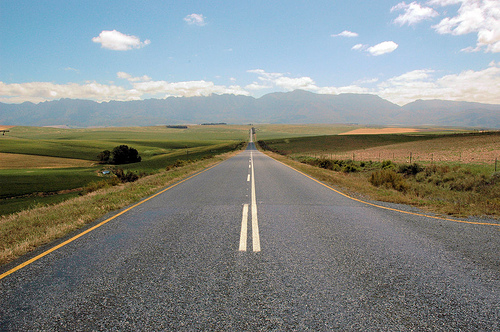
\includegraphics[width=0.5\textwidth]{photos/roadby_cornstaruk_flickr.jpg}
\end{center}
\end{Investigation}



\section{Versnelling}
\Definition{Gemiddelde versnelling} {Gemiddelde versnelling is die verandering in gemiddelde snelheid gedeel deur die tyd wat geneem is.\\
Simbool: $\vec{a}_{av}$\hspace{2cm} S.I. Eenhede: $\text{m} \cdot \text{s}^{-2}$ } 

Versnelling is 'n mate van hoe vinnig  die snelheid van 'n voorwerp oor tyd verander. As ons 'n verander in snelheid ($\Delta \vec{v}$) het, oor 'n tydsinterval ($\Delta t$), dan word die gemiddelde versnelling ($\vec{a}_{av}$) gedefini\"eer as:

\begin{equation*}
    \text{gemiddelde versnelling (in m} \cdot {\text{s}}^{-2}\text{)} =\frac{\text{verandering in snelheid (in m} \cdot {\text{s}}^{-1}\text{)}}{\text{verandering in tyd (in s)}}
      \end{equation*}
        
    \begin{equation*}
    \vec{a}_{av}=\frac{\Delta \vec{v}}{\Delta t}
      \end{equation*}

Ons werk net met probleme wat konstante versnelling behels. Dit beteken dat die gemiddelde versnelling en die oombliklike versnelling diselfde is. Om dinge makliker te maak sal ons net praat van versnelling en nie ``gemiddeld'' of ``oombliklik'' nie. Dit word as $\vec{a}$ voorgstel. Ons het ook die grootte van die versnelling. Dit is:
\begin{equation*}
    a=\frac{\Delta \vec{v}}{\Delta t}
\end{equation*}

Versnelling is 'nm vektor. Versnelling s\^e niks van die beweging nie maar net hoe vinnig die bewegin verander. Dit is nie moontlik om te s\^e hoe vinnig 'n voorwerp beweeg of in watter rigting dit beweeg van die snelheid aleenlik nie.\par \mindsetvid{Acceleration}{VPgly}


Soos snelheid, kan versnelling ook positief of negatief wees. Wanneer die teken van die versnelling en die snelheid dieselfde is, beweeg die voorwerp al hoe vinniger. As die beide die versnelling en snelheid positief is, beweeg die voorwerp al hoe vinniger in die positiewe rigting. Netso, as beide negatief is beweeg die voorwerp die al hoe vinniger in die negatiewe rigting.      

\Tip{Vermy die woord \textsl{vertraging} as jy na 'n negatiewe versnelling verwys. Dit beteken gewoonlik \textsl{vermindering in spoed} maar dit is moontlik vir 'n voorwerp om spoed te verminder met beide 'n positiewe of negatiewe versnelling, want die teken van die snelheid moet ook in ag geneem word om vas te stel of 'n voorwerp spoed verminder of nie.}

Ons kan dit sien in die volgende diagram:
\begin{figure}[H]
 \begin{center}
  \begin{pspicture}(-5,-1)(5,3)
\rput(-3,0){
\pspolygon(0,0)(0,1)(1,1)(1,0)(0,0)
\psline{->}(0.3,1.1)(0.9,1.1)
\rput[tl](0.3,1.5){$\vec{v}$}
\psline{->}(0.5,0.5)(1.5,0.5)
\rput[tr](1.5,0.3){$\vec{a}$}
\rput(.8,-.3){beweeg vinniger}}
\rput(-0.5,0){
\pspolygon(0,0)(0,1)(1,1)(1,0)(0,0)
\psline{<-}(0.3,1.1)(0.9,1.1)
\rput[tl](0.3,1.5){$\vec{v}$}
\psline{->}(0.5,0.5)(1.5,0.5)
\rput[tr](1.5,0.3){$\vec{a}$}
\rput(.8,-.3){beweeg stadiger}
}
\rput(3,0){
\pspolygon(0,0)(0,1)(1,1)(1,0)(0,0)
\psline{<-}(0.3,1.1)(0.9,1.1)
\rput[tl](0.3,1.5){$\vec{v}$}
\psline{->}(0.5,0.5)(-0.5,0.5)
\rput[tr](-.5,0.3){$\vec{a}$}
\rput(.8,-.3){beweeg vinniger}
\rput(.8,-.6){negatiewe versnelling}}
  \end{pspicture}
 \end{center}
\end{figure}

As snelheid positief is en versnelling is negatief, dan sal die voorwerp se spoed verminder. Op dieselfde manier, as die snelheid negatief en die versnelling positief is, sal die voorwerp se spoed verminder. Dit word in die volgende voorbeeld illustreer.

\begin{wex}{Versnelling}{'n Kar versnel eenvormig van 'n aanvanklike snelheid van 2 m$\cdot$s$^{-1}$ tot 'n finale snelheid van 10 m$\cdot$s$^1$ in 8 sekondes. Dit verminder dan spoed teen 'n egalige tempo tot 'n finale snelheid van 4 m$\cdot$s$^{-1}$ in 6 sekondes. Bereken die versnelling van die kar gedurende die eerste 8 sekondes en gedurende die laaste 6 sekondes.}
{
\westep{Kies 'n verwysingsraamwerk}
Ons kies die punt waar die kar sy versnelling begin as die oorsproing en die rigting waarin hy alreeds beweeg as die positiewe rigting.
\westep{Identifiseer watter inligting gegee is en wat gevra word}
Beskou die beweging van die kar in twee dele: die eerste 8 sekondes en die laaste 6 sekondes.\\

\begin{minipage}{0.5\textwidth}
\center{Vir die eerste 8 sekondes:}
\begin{eqnarray*}
\vec{v}_i &=& 2~\text{m}\cdot \text{s}^{-1}\\
\vec{v}_f &=& 10~\text{m}\cdot \text{s}^{-1}\\
t_i &=& 0~\text{s}\\
t_f &=& 8~\text{s}
\end{eqnarray*}
\end{minipage}
\begin{minipage}{0.5\textwidth}
\center{Vir die laaste 6 sekondes:}
\begin{eqnarray*}
\vec{v}_i &=& 10~\text{m}\cdot \text{s}^{-1}\\
\vec{v}_f &=& 4~\text{m}\cdot \text{s}^{-1}\\
t_i &=& 8~\text{s}\\
t_f &=& 14~\text{s}
\end{eqnarray*}

\end{minipage}\\

\westep{Bereken die versnelling}
\begin{minipage}[t]{0.5\textwidth}
\center{Vir die eerste 8 sekondes:}
\begin{eqnarray*}
a &=& \frac{\Delta v}{\Delta t}\\
&=& \frac{10\textrm{ \text{m}\cdot \text{s}^{-1}} - 2\textrm{ \text{m}\cdot \text{s}^{-1}}}{8\textrm{ s} - 0\textrm{ s}}\\
&=& 1~\text{m}\cdot \text{s}^{-2}
\end{eqnarray*}

\end{minipage}
\begin{minipage}[t]{0.5\textwidth}
\center{Vir die laaste 6 sekondes:}
\begin{eqnarray*}
a &=& \frac{\Delta v}{\Delta t}\\
&=& \frac{4\textrm{ \text{m}\cdot \text{s}^{-1}} - 10\textrm{ \text{m}\cdot \text{s}^{-1}}}{14\textrm{ s} - 8\textrm{ s}}\\
&=& -1~\text{m}\cdot \text{s}^{-2}
\end{eqnarray*}

\end{minipage}\\
Gedurende die eerste 8 sekondes het die kar 'n positiewe versnelling. Die kar se snelheid is ook positief en dus vermeerder die kar se spoed.\par
Gedurende die volgende 6 sekondes het die kar 'n negatiewe versnelling maar 'n positiewe snelheid. Dit beteken die kar verminder spoed.
}
\end{wex}


\begin{exercises}{Versnelling}
      
\noindent
\begin{enumerate}[noitemsep, label=\textbf{\arabic*}. ] 
    \item 'n Atleet versnel eenvormig van 'n aanvanklike snelheid van 0 m$\ensuremath{\cdot}$s${}^{-1}$ tot 'n finale snelheid van 4 m$\ensuremath{\cdot}$s${}^{-1}$ in 2 sekondes. Bereken sy versnelling. Maak die rigting waarin die atleet hardloop positief.    
    \item \n Bus versnel eenvormig van 'n aanvanklike snelheid van 15 m$\ensuremath{\cdot}$s${}^{-1}$ tot 'n finale snelheid van 7~m$\ensuremath{\cdot}$s${}^{-1}$ in 4 sekondes. Bereken die versnelling van die bus. Maak die rigting waarin die bus beweeg positief.

    \item 'n Vliegtuig versnel eenvormig van 'n snelheid van 200 m$\ensuremath{\cdot}$s${}^{-1}$ tot 'n snelheid van100 m$\ensuremath{\cdot}$s${}^{-1}$in 10 sekondes. Dit versnel dan eenvormig tot 'n finale snelheid van 240 m$\ensuremath{\cdot}$s${}^{-1}$in 20 sekondes. Maak die rigting waarin die vliegtuig beweeg positief.
 
    \begin{enumerate}[noitemsep, label=\textbf{\alph*}. ] 
            \item Bereken die versnelling van die vliegtuig gedurende die eerste 10 sekondes.
            \item Bereken die versnelling van die vliegtuig gedurende die volgende 14 sekondes.
    \end{enumerate}
\end{enumerate}
\practiceinfo
\par \begin{tabular}[h]{cccccc}
(1.) l1k  &  (2.) l10  &  (3.) l18  & \end{tabular}
\end{exercises}


\section{Oombliklike snelheid en spoed}


\begin{minipage}{.5\textwidth}
\begin{center}
\textbf{Naellopers spring weg}\\
\includegraphics[width=.8\textwidth]{photos/sprintersstarting_wwarby_flickr.jpg}\\
\textbf{Einde van resies}\\
\includegraphics[width=.8\textwidth]{photos/sprintersending_wwarby_flickr.jpg}\\
\textit{Fotos deur wwarby op Flickr.}
\end{center}
\end{minipage}
\begin{minipage}{.5\textwidth}

Ons het gekyk na die gemiddelde snelheid en spoed maar soms wil ons meer presies weet wat gebeur tussen die aanvanklike en finale tye in 'n probleem.

Oombliklike snelheid is die snelheid op 'n spesifieke tyd. Dit kan anders wees as die gemiddelde snelheid as die snelheid nie konstant is nie.

Kyk na die fotos van die naellopers in 'n wedloop. Hul snelheid by die wegspring is anders as aan die einde van die resies. Hulle gemiddelde snelheid vir die resies verander nie maar hulle oombklilike snelheid, soos vasgevang in die fotos op 'n sekere tyd, verander wel. Die snelheid van die naelloper toe die die foto geneem is, is sy oombliklike snelheid.

\end{minipage}

\Tip{'n Oomblik in tyd is anders as die tyd geneem of 'n tydsinterval. Dit is dus handig om die simbool $t$ te gebruik vir 'n oomblik in tyd (byvoorbeeld gedurende die 4$^\text{e}$ sekonde) en die simbool $\Delta t$ vir 'n tydsinterval (byvoorbeeld die eerste 5 sekondes van die beweging).}\\


\Definition{Oombliklike snelheid}{Oombliklike snelheid is die verandering in posisie oor die verandering in 'n bye kort tydsinterval. ($\Delta t \approx 0$). \\
Simbool: $\vec{v}$\hspace{2cm} S.I. Eenhede: $\text{m}\cdot \text{s}^{-1}$} 

\Definition{Oombliklike spoed}{Oombliklike spoed is die grootte van oombliklike snelheid.\\
Symbol: $v$\hspace{2cm} S.I. Units: $\text{m}\cdot \text{s}^{-1}$} 

Oombliklike snelheid is 'n vektor. Oombliklike spoed is die grootte van oombliklike snelheid. Die het dieselfde waarde maar het nie 'n rigting nie en is dus nie 'n vektor nie.


\section{Beskrywing van beweging}
%NTS this section needs a formal project on acceleration

Die doel van hierdie hoofstuk is om beweging te beskryf en nou dat ons die definisies van verplasing, afstand, snelheid, spoed en versnelling verstaan, is ons gereed om hierdie idees te gebruik om te beskryf hoe 'n voorwerp of persoon beweeg. Ons sal na drie maniere  om beweging te beskryf kyk:\par 
\begin{enumerate}[noitemsep, label=\textbf{\arabic*}. ] 
    \item woorde
    \item diagramme
    \item grafieke
\end{enumerate}
Hierdie metodes sal in die volgende seksie beskryf word. \par 
Ons sal drie soorte beweging beskou: wanneer 'n voorwerp nie beweeg nie (stilstaande voorwerp), wanneer 'n voorwerp teen 'n konstante snelheid bweeg (eenvormige beweging) en wanneer 'n voorwerp teen 'n konstante tempo versnel (beweging teen konstante versnelling).\par 

\subsection*{Stilstaande Voorwerpe}
\nopagebreak
Die eenvoudigste bewegin wat ons te\"e kom is di\'e van 'n stilstaande voorwerp. 'n Stilstaande voorwerp beweeg nie en sy posisie verander nie.

\begin{minipage}{.5\textwidth}
Beskou die volgende voorbeeld. Vivian wag vir 'n taxi. Sy staan twee meter vanaf 'n stopstraat by $t=0~\text{s}$. Na een minuut, by $t=60~\text{s}$, staan sy nog steeds 2 meter van die stopstraat en na twee minute, by $t=120~\text{s}$ staan sy ook  2 meter vanaf die stopstraat. Haar posisie het nie verander nie. Haar verplasing is nul (want haar posisie is nog dieselfde), haar snelheid is nul want haar verplasing is nul en haar versnelling is ook nul (want haar snelheid het nie verander nie ).

Ons kan nou grafieke trek van posisie teen tyd ($\vec{x}$ vs. $t$), snelheid teen tyd ($\vec{v}$ vs. $t$) en versnelling teen tyd ($\vec{a}$ vs. $t$) vir 'n stilstaande voorwerp. Die grafieke word hieronder gewys.
\end{minipage}
\begin{minipage}{.5\textwidth}
\begin{center}
 \textbf{Vivian staan by 'n stopstraat.}\\
%\includegraphics[width=.8\textwidth]{photos/stopstreet_by_CarolynColes_Flickr.jpg}\\
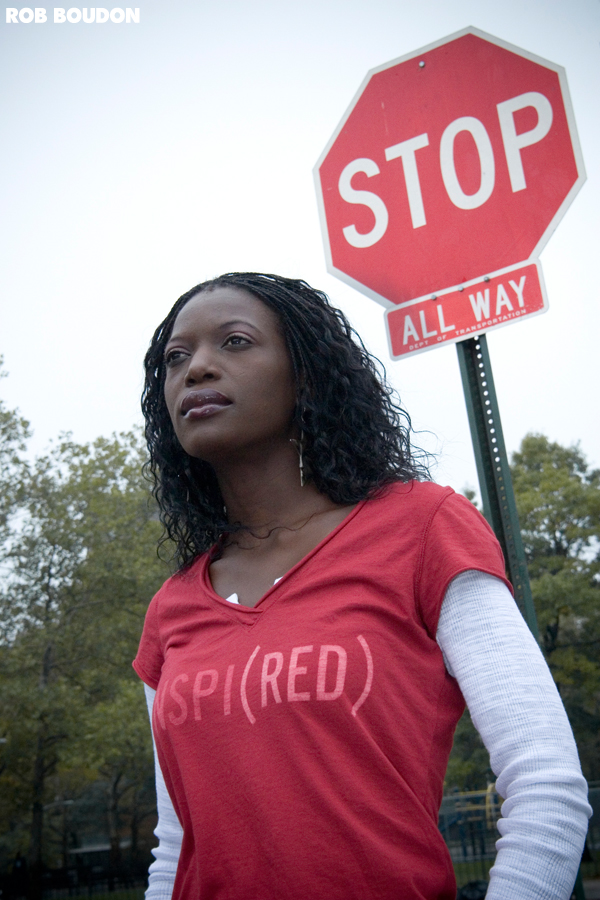
\includegraphics[width=.8\textwidth]{photos/stopstreet_by_RobBoudon_Flickr.jpg}\\
\textit{Foto deur Rob Boudon op Flickr}
\end{center}
\end{minipage}



\begin{center}
\scalebox{1} % Change this value to rescale the drawing.
{
\begin{pspicture}(0,-2.3034375)(15.0207815,2.3034375)

\rput(9.671615,2.3734374){   }
\psline[]{->}(0.79578125,-1.1865625)(0.79578125,1.8134375)
\psline[]{->}(0.79578125,-1.1865625)(3.7957811,-1.1865625)
\psline[]{->}(5.795781,-1.1865625)(5.795781,1.8134375)
\psline[]{->}(5.795781,-1.1865625)(8.795781,-1.1865625)
\psline[]{->}(10.795781,-1.1865625)(10.795781,1.8134375)
\psline[]{->}(10.795781,-1.1865625)(13.795781,-1.1865625)
\psline[linewidth=0.09cm](10.795781,-1.1865625)(12.795781,-1.1865625)
\psline[linewidth=0.09cm](5.795781,-1.1865625)(7.795781,-1.1865625)
\psline[linewidth=0.09cm](0.79578125,0.8134375)(2.7957811,0.8134375)

\rput(1.7615625,-1.4765625){60}

\rput(2.8382812,-1.4765625){120}

\rput(0.574375,0.8234375){2}

\rput(0.54265624,-0.1765625){1}

\rput(0.5728125,-1.2765625){0}

\rput(7.838281,-1.4765625){120}

\rput(12.738281,-1.4765625){120}
\psline[](1.7957813,-1.0865625)(1.7957813,-1.1865625)
\psline[](2.7957811,-1.0865625)(2.7957811,-1.1865625)
\psline[](6.795781,-1.0865625)(6.795781,-1.1865625)
\psline[](7.795781,-1.0865625)(7.795781,-1.1865625)
\psline[](11.795781,-1.0865625)(11.795781,-1.1865625)
\psline[](12.795781,-1.0865625)(12.795781,-1.1865625)
\psline[](0.69578123,-0.1865625)(0.8957813,-0.1865625)
\psline[](0.69578123,0.8134375)(0.79578125,0.8134375)

\rput(4.4365625,-1.1765625){tyd(s)}

\rput(9.436563,-1.1765625){tyd (s)}

\rput(14.436563,-1.1765625){tyd (s)}

\rput{-270.0}(0.571875,0.2365625){\rput(0.16890626,0.4234375){posisie $x$ (m)}}

\rput{-270.0}(5.9035935,-5.0960937){\rput(5.496719,0.4234375){snelheid $v$ (\ms)}}

\rput{-270.0}(10.958906,-10.150469){\rput(10.541875,0.4234375){versnelling $a$ (m$\cdot$s$^{-2}$)}}

\rput(5.6728125,-1.2765625){0}

\rput(10.672812,-1.2765625){0}

\rput(6.7615623,-1.4765625){60}

\rput(11.761562,-1.4765625){60}

\rput(1.9809375,-2.0765624){(a)}

\rput(6.9909377,-2.0765624){(b)}

\rput(11.980938,-2.0765624){(c)}
\psline[](2.7957811,0.8134375)(2.7957811,-1.0865625)
\end{pspicture} 
}
\caption{Grafieke vir 'n stilstaande voorwerp (a) posisie teen tyd (b) snelheid teen tyd (c) versnelling teen tyd.}
\label{fig:pr:stationary}
\end{center}

Vivian se posisie is 2~meter vanaf die stopstraat as die stopteken as die verwysingspunt geneem word. Haar posisie bly 2~meter vir 120~sekondes. Die grafiek is 'n horisontale lyn by $2 \text{ m}$. Die snelheid en versnelling grafieke word ook gewys. Hulle is albei horisontale lyne op die $x$-as. Omdat haar posisie nie verander nie, is haar snelheid $0~\text{m}\ensuremath{\cdot}\text{s}{}^{-1}$ en omdat haar snelheid nie verander nie, is haar versnelling $0~\text{m}\ensuremath{\cdot}\text{s}{}^{-2}$.\par 


\par
\Definition{Gradi\"ent} {Die gradi\"ent, $m$, van 'n lyn kan bereken word deur die verandering in die $y$ waarde (afhanklike veranderlike) te deel deur die verandering in die $x$ waarde (onafhanklike veranderlike) $$m = \frac{\Delta y}{\Delta x}$$ \par  } 

Omdat ons weet dat snelheid die tempo van verandering van posisie is, kan ons die waarde van die snelheid teen tyd grafiek bevesting deur die gradi\"ent van die $\vec{x}$ vs. $t$ grafiek te bereken.\par 

\Tip{Die gradi\"ent van 'n posisie teen tyd grafiek gee die snelheid.}
	\par
As ons die gradi\"ent van die $\vec{x}$~vs.~$t$ grafiek van 'n stilstaande voorwerp bereken, kry ons:\par 
        \label{m38795*id69332}\nopagebreak\noindent{}
    \begin{align*}
	v &= \frac{\Delta \vec{x}}{\Delta t}\\
	&= \frac{\vec{x}_{f}-\vec{x}_{i}}{{t}_{f}-{t}_{i}}\\
	&= \frac{2~\text{m}-2~\text{m}}{120~\text{s}-60~\text{s}} \left(\text{aanvanklike\; posisie}=\text{finale\; posisie}\right)\\ 
	&= 0~\text{m}\ensuremath{\cdot}{\text{s}}^{-1}  \left(\text{gedurende\; die \; tyd\; wat\; Vivian\; stilstaande\; is}~\right) \\
      \end{align*}
Op 'n soortgelyke manier kan ons die waarde van die versnelling bevestig deur die gradi\"ent van die snelheid teen tyd grafiek te bereken.\par 

\Tip{Die gradi\"ent van 'n snelheid teen tyd grafiek is die versnelling.}
	\par
As ons die gradi\"ent van die $\vec{v}$ vs. $t$ grafiek van 'n stilstaande voorwerp bereken, kry ons:\par 
        \label{m38795*id69594}\nopagebreak\noindent{}
          
    \begin{align*}
    a &= \frac{\Delta v}{\Delta t}\hfill \\ 
    &= \frac{\vec{v}_{f}-\vec{v}_{i}}{{t}_{f}-{t}_{i}}\hfill \\ 
    &= \frac{0~\text{m}\cdot\text{s}^{-1}-0~\text{m}\cdot\text{s}^{-1}}{120~\text{s}-60~\text{s}}\\ 
    &= 0~\text{m}\cdot\text{s}^{-2}
      \end{align*}

Daarbenewens, omdat die snelheid teen tyd grafiek verwant is aan die posisie teen tyd grafiek, kan ons die oppervlak onder die snelheid teen tyd grafiek gebruik om die verplasing van 'n voorwerp te bereken.\par 

\Tip{Die oppervlak onder die snelheid teen tyd grafiek gee die verplasing.}
	\par

Die verplasing van die voorwerp word gegee deur die oppervlak onder die grafiek, wat $0~\text{m}$ is. Dit is voor die hand liggend want die voorwerp beweeg nie.\par 


\subsection*{Beweging teen konstante snelheid}
\nopagebreak
Beweging teen 'n konstante snelheid of \textsl{eenvormige beweging} beteken dat die posisie van 'n voorwerp teen 'n konstante tempo verander.\par 
Neem aan dat dit Vivian $100~\text{s}$ vat om die $100~\text{m}$ na die taxi-stop af te l\^e. As ons aanneem dat Vivian se huis die oorsprong is, dan is Vivian se snelheid:\par 
        \label{m38795*id69850}\nopagebreak\noindent{}
          
    \begin{align*}
    	v&= \frac{\Delta \vec{x}}{\Delta t}\hfill \\ 
	&= \frac{{x}_{f}-{x}_{i}}{{t}_{f}-{t}_{i}}\hfill \\ 
	&= \frac{100~\text{m}-0~\text{m}}{100~\text{s}-0~\text{s}}\\ 
	 &= 1~\text{m}\cdot{\text{s}}^{-1}
      \end{align*}
Vivian se snelheid is 1 m$\ensuremath{\cdot}$s${}^{-1}$. Dit beteken dat sy $1~\text{m}$ gestap het in die eerste sekonde, nog 'n meter in die tweede sekonde, en nog 'n meter in die derde sekonde ensovoorts. Byvoorbeeld, na $50~\text{s}$ sal sy $50~\text{m}$ van die huis af wees.from home. Haar posisie vermeerder met $1~\text{m}$ elke $1~\text{s}$. 'n Diagram van Vivian se posisie word hieronder gewys:\par 

\begin{center}
\scalebox{1} % Change this value to rescale the drawing.
{
\begin{pspicture}(0,-1.57375)(9.02,1.53375)
\psline[]{->}(2.0,-0.46625)(9.0,-0.46625)
\psframe[linewidth=0.04,dimen=outer](2.0,0.53375)(0.0,-0.46625)
\pstriangle[linewidth=0.04,dimen=outer](1.0,0.53375)(2.0,1.0)
\psframe[linewidth=0.04,dimen=outer](1.2,0.23375)(0.8,-0.46625)
\psframe[linewidth=0.04,dimen=outer](1.8,0.23375)(1.4,-0.06625)
\psframe[linewidth=0.04,dimen=outer](0.6,0.23375)(0.2,-0.06625)
\psellipse[linewidth=0.04,dimen=outer](2.15,0.53375)(0.15,0.2)
\psline[](2.1,0.33375)(2.1,0.33375)
\psline[linewidth=0.051999997cm](2.14,0.37375)(2.14,-0.02625)
\psline[](2.14,-0.02625)(2.24,-0.24625)
\psline[](2.24,-0.24625)(2.2,-0.42625)
\psline[](2.2,-0.42625)(2.3,-0.42625)
\psline[](2.12,-0.00625)(2.1,-0.26625)
\psline[](2.1,-0.26625)(2.02,-0.42625)
\psline[](2.02,-0.42625)(2.12,-0.42625)
\psline[](2.12,0.27375)(2.04,0.03375)
\psline[](2.04,0.03375)(2.22,0.15375)
\psline[](2.12,0.21375)(2.24,-0.02625)
\psline[](2.24,-0.02625)(2.32,0.03375)
\psdots[dotsize=0.04](2.2,0.59375)
\pscustom[linewidth=0.04]
{
\newpath
\moveto(2.12,0.51375)
\lineto(2.17,0.47375)
\curveto(2.195,0.45375)(2.225,0.43875)(2.24,0.45375)
}
\pscustom[linewidth=0.04]
{
\newpath
\moveto(2.24,0.69375)
\lineto(2.19,0.70375)
\curveto(2.165,0.70875)(2.12,0.70875)(2.1,0.70375)
\curveto(2.08,0.69875)(2.05,0.67875)(2.04,0.66375)
\curveto(2.03,0.64875)(2.015,0.62875)(2.0,0.61375)
}
\pscustom[linewidth=0.04]
{
\newpath
\moveto(2.0,0.61375)
\lineto(2.03,0.64375)
\curveto(2.045,0.65875)(2.08,0.67875)(2.1,0.68375)
\curveto(2.12,0.68875)(2.165,0.69375)(2.19,0.69375)
\curveto(2.215,0.69375)(2.245,0.68375)(2.26,0.65375)
}
\pscustom[linewidth=0.04]
{
\newpath
\moveto(2.14,0.71375)
\lineto(2.1,0.67375)
\curveto(2.08,0.65375)(2.055,0.61875)(2.04,0.57375)
}

\rput[l](8,-1.05625){$x$ = 100 m}

\rput[l](2,-0.73625){t = 0 s}

\rput[l](5,-0.73625){t = 50 s}

\rput[l](8,-0.73625){t = 100 s}

\rput[l](5,-1.05625){$x$ = 50 m}

\rput[l](2,-1.05625){$x$ = 0 m}
\psline[](5.0,1.07375)(5.0,-0.44625)
\psline[](7.98,1.05375)(7.98,-0.46625)
\psellipse[linewidth=0.04,dimen=outer](5.17,0.51375)(0.15,0.2)
\psline[](5.12,0.31375)(5.12,0.31375)
\psline[linewidth=0.051999997cm](5.16,0.35375)(5.16,-0.04625)
\psline[](5.16,-0.04625)(5.26,-0.26625)
\psline[](5.26,-0.26625)(5.22,-0.44625)
\psline[](5.14,-0.02625)(5.12,-0.28625)
\psline[](5.12,-0.28625)(5.04,-0.44625)
\psline[](5.14,0.25375)(5.06,0.01375)
\psline[](5.06,0.01375)(5.24,0.13375)
\psline[](5.14,0.19375)(5.26,-0.04625)
\psline[](5.26,-0.04625)(5.34,0.01375)
\psdots[dotsize=0.04](5.22,0.57375)
\pscustom[linewidth=0.04]
{
\newpath
\moveto(5.14,0.49375)
\lineto(5.19,0.45375)
\curveto(5.215,0.43375)(5.245,0.41875)(5.26,0.43375)
}
\pscustom[linewidth=0.04]
{
\newpath
\moveto(5.26,0.67375)
\lineto(5.21,0.68375)
\curveto(5.185,0.68875)(5.14,0.68875)(5.12,0.68375)
\curveto(5.1,0.67875)(5.07,0.65875)(5.06,0.64375)
\curveto(5.05,0.62875)(5.035,0.60875)(5.02,0.59375)
}
\pscustom[linewidth=0.04]
{
\newpath
\moveto(5.02,0.59375)
\lineto(5.05,0.62375)
\curveto(5.065,0.63875)(5.1,0.65875)(5.12,0.66375)
\curveto(5.14,0.66875)(5.185,0.67375)(5.21,0.67375)
\curveto(5.235,0.67375)(5.265,0.66375)(5.28,0.63375)
}
\pscustom[linewidth=0.04]
{
\newpath
\moveto(5.16,0.69375)
\lineto(5.12,0.65375)
\curveto(5.1,0.63375)(5.075,0.59875)(5.06,0.55375)
}
\psellipse[linewidth=0.04,dimen=outer](8.13,0.55375)(0.15,0.2)
\psline[](8.08,0.35375)(8.08,0.35375)
\psline[linewidth=0.051999997cm](8.12,0.39375)(8.12,-0.00625)
\psline[](8.1,0.01375)(8.08,-0.24625)
\psline[](8.1,0.29375)(8.02,0.05375)
\psline[](8.02,0.05375)(8.2,0.17375)
\psline[](8.1,0.23375)(8.22,-0.00625)
\psline[](8.22,-0.00625)(8.3,0.05375)
\psdots[dotsize=0.04](8.18,0.61375)
\pscustom[linewidth=0.04]
{
\newpath
\moveto(8.1,0.53375)
\lineto(8.15,0.49375)
\curveto(8.175,0.47375)(8.205,0.45875)(8.22,0.47375)
}
\pscustom[linewidth=0.04]
{
\newpath
\moveto(8.22,0.71375)
\lineto(8.17,0.72375)
\curveto(8.145,0.72875)(8.1,0.72875)(8.08,0.72375)
\curveto(8.06,0.71875)(8.03,0.69875)(8.02,0.68375)
\curveto(8.01,0.66875)(7.995,0.64875)(7.98,0.63375)
}
\pscustom[linewidth=0.04]
{
\newpath
\moveto(7.98,0.63375)
\lineto(8.01,0.66375)
\curveto(8.025,0.67875)(8.06,0.69875)(8.08,0.70375)
\curveto(8.1,0.70875)(8.145,0.71375)(8.17,0.71375)
\curveto(8.195,0.71375)(8.225,0.70375)(8.24,0.67375)
}
\pscustom[linewidth=0.04]
{
\newpath
\moveto(8.12,0.73375)
\lineto(8.08,0.69375)
\curveto(8.06,0.67375)(8.035,0.63875)(8.02,0.59375)
}
\psline[](8.14,-0.44625)(8.22,-0.44625)
\psline[](8.02,-0.44625)(8.1,-0.44625)
\psline[](8.12,-0.00625)(8.22,-0.22625)
\psline[](8.08,-0.22625)(8.02,-0.44625)
\psline[](8.22,-0.20625)(8.14,-0.44625)
\psline[](5.02,-0.42625)(5.12,-0.42625)
\psline[](5.2,-0.42625)(5.28,-0.42625)

\rput[l](5,-1.37625){$v$ = 1\text{m}\cdot \text{s}^{-1}}

\rput[l](8,-1.39625){$v$ = 1\text{m}\cdot \text{s}^{-1}}
\end{pspicture} 
}
\end{center}
\caption{Diagram van Vivian se beweging teen 'n konstante snelheid van 1 \text{m}\cdot \text{s}^{-1} wys.}
\label{fig:pr:diagram:uniform}

Ons kan nou grafieke van posisie teen tyd ($\vec{x}$ vs. $t$), snelheid teen tyd ($\vec{v}$ vs. $t$) en versnelling teen tyd ($\vec{a}$ vs. $t$) teken vir Vivian se beweging teen 'n konstante snelheid. Die grafieke word hier gewys:
\begin{center}
\scalebox{1} % Change this value to rescale the drawing.
{
\begin{pspicture}(0,-2.3034375)(15.220781,2.3034375)
\definecolor{color1158b}{rgb}{0.8,0.8,0.8}

\rput(9.871614,2.3734374){   }
\psline[]{->}(0.99578124,-1.1865625)(0.99578124,1.8134375)
\psline[]{->}(0.99578124,-1.1865625)(3.9957812,-1.1865625)
\psline[]{->}(5.9957814,-1.1865625)(5.9957814,1.8134375)
\psline[]{->}(5.9957814,-1.1865625)(8.995781,-1.1865625)
\psline[]{->}(10.995781,-1.1865625)(10.995781,1.8134375)
\psline[]{->}(10.995781,-1.1865625)(13.995781,-1.1865625)
\psline[linewidth=0.09cm](10.995781,-1.1865625)(12.995781,-1.1865625)
\psline[linewidth=0.09cm](5.9957814,-0.1865625)(7.9957814,-0.1865625)
\psline[linewidth=0.09cm](0.99578124,-1.1865625)(2.9957812,0.8134375)

\rput(1.9607812,-1.4765625){50}

\rput(3.0382812,-1.4765625){100}

\rput(0.53828126,0.8234375){100}

\rput(0.66078126,-0.1765625){50}

\rput(0.7728125,-1.2765625){0}

\rput(8.038281,-1.4765625){100}

\rput(12.938281,-1.4765625){100}
\psline[](1.9957813,-1.0865625)(1.9957813,-1.1865625)
\psline[](2.9957812,-1.0865625)(2.9957812,-1.1865625)
\psline[](6.9957814,-1.0865625)(6.9957814,-1.1865625)
\psline[](7.9957814,-1.0865625)(7.9957814,-1.1865625)
\psline[](11.995781,-1.0865625)(11.995781,-1.1865625)
\psline[](12.995781,-1.0865625)(12.995781,-1.1865625)
\psline[](0.8957813,-0.1865625)(1.0957812,-0.1865625)
\psline[](0.8957813,0.8134375)(0.99578124,0.8134375)

\rput(4.6365623,-1.1765625){tyd (s)}

\rput(9.636562,-1.1765625){tyd (s)}

\rput(14.636562,-1.1765625){tyd (s)}

\rput{-270.0}(0.571875,0.2365625){\rput(0.16890626,0.4234375){posisie $x$ (m)}}

\rput{-270.0}(5.8035936,-4.9960938){\rput(5.396719,0.4234375){snelheid $v$ (\ms)}}

\rput{-270.0}(11.0,-10.350469){\rput(10.741875,0.4234375){versnelling $a$ (m$\cdot$s$^{-2}$)}}

\rput(5.8728123,-1.2765625){0}

\rput(10.872812,-1.2765625){0}

\rput(6.960781,-1.4765625){50}

\rput(11.960781,-1.4765625){50}

\rput(2.1809375,-2.0765624){(a)}

\rput(7.1909375,-2.0765624){(b)}

\rput(12.180938,-2.0765624){(c)}
\psline[](2.9957812,0.8134375)(2.9957812,-1.0865625)

\rput(5.742656,-0.1765625){1}
\psline[](5.895781,-0.1865625)(6.0957813,-0.1865625)
\psline[](2.8957813,0.8134375)(0.99578124,0.8134375)
\psline[](7.9957814,-0.1865625)(7.9957814,-1.1865625)
\psframe[linewidth=0.02,linecolor=color1158b,dimen=outer,fillstyle=solid,fillcolor=color1158b](7.9757814,-0.2265625)(6.0157814,-1.1465625)
\psline[linewidth=0.03cm,](2.5757813,0.3534375)(2.5757813,-0.5865625)
\psline[linewidth=0.03cm,](2.5757813,-0.5865625)(1.6357813,-0.5865625)
\rput[l](2.7,-0.1365625){$\Delta$x}
\rput(2.2054687,-0.7315625){\footnotesize $\Delta$t}
\end{pspicture} 
}
\caption{Grafieke vir konstante snelheid (a) posisie teen tyd (b) snelheid teen tyd (c) versnelling teen tyd. Die oppervlak van die ingekleurde deel in die $v$ vs. $t$ grafiek stem ooreen met die voorwerp se verplasing.}
\label{fig:pr:uniform}
\end{center}

In die aand loop Vivian $100~\text{m}$ van die busstop to by haar huis in $100~\text{s}$. Ons neem aan Vivian se huis is die oorsprong. Die volgende grafieke kan geteken word om die beweging te beskryf.\par 
\begin{center}
\scalebox{1} % Change this value to rescale the drawing.
{
\begin{pspicture}(0,-2.3034375)(15.220781,2.3034375)
\definecolor{color1158b}{rgb}{0.8,0.8,0.8}

\rput(9.871614,2.3734374){   }
\psline[]{->}(0.99578124,-1.1865625)(0.99578124,1.8134375)
\psline[]{->}(0.99578124,-1.1865625)(3.9957812,-1.1865625)
\psline[]{<->}(6.0110865,1.8133594)(5.980476,-1.1864845)
\psline[]{->}(5.9957814,0.8134375)(8.995781,0.8134375)
\psline[]{->}(10.995781,-1.1865625)(10.995781,1.8134375)
\psline[]{->}(10.995781,-1.1865625)(13.995781,-1.1865625)
\psline[linewidth=0.09cm](10.995781,-1.1865625)(12.995781,-1.1865625)
\psline[linewidth=0.09cm](5.9957814,-0.1865625)(7.9957814,-0.1865625)
\psline[linewidth=0.09cm](0.97578126,0.8134375)(2.9957812,-1.1865625)

\rput(1.9607812,-1.4765625){50}

\rput(3.0382812,-1.4765625){100}

\rput(0.53828126,0.8234375){100}

\rput(0.66078126,-0.1765625){50}

\rput(0.7728125,-1.2765625){0}

\rput(7.938281,1.0234375){100}

\rput(12.938281,-1.4765625){100}
\psline[](1.9957813,-1.0865625)(1.9957813,-1.1865625)
\psline[](2.9957812,-1.0865625)(2.9957812,-1.1865625)
\psline[](6.9957814,0.9134375)(6.9957814,0.8134375)
\psline[](7.9957814,0.9134375)(7.9957814,0.8134375)
\psline[](11.995781,-1.0865625)(11.995781,-1.1865625)
\psline[](12.995781,-1.0865625)(12.995781,-1.1865625)
\psline[](0.8957813,-0.1865625)(1.0957812,-0.1865625)
\psline[](0.8957813,0.8134375)(0.99578124,0.8134375)

\rput(4.6365623,-1.1765625){tyd (s)}

\rput(9.536563,0.8234375){tyd (s)}

\rput(14.636562,-1.1765625){tyd (s)}

\rput{-270.0}(0.571875,0.2365625){\rput(0.16890626,0.4234375){posisie $x$ (m)}}

\rput{-270.0}(5.8035936,-4.9960938){\rput(5.396719,0.4234375){snelheid $v$ (\ms)}}

\rput{-270.0}(11.158906,-10.350469){\rput(10.741875,0.4234375){versnelling $a$ (m$\cdot$s$^{-2}$)}}

\rput(5.7728124,0.8234375){0}

\rput(10.872812,-1.2765625){0}

\rput(6.960781,1.0234375){50}

\rput(11.960781,-1.4765625){50}

\rput(2.1809375,-2.0765624){(a)}

\rput(7.1909375,-2.0765624){(b)}

\rput(12.180938,-2.0765624){(c)}

\rput(5.7164063,-0.1765625){-1}
\psline[](5.895781,-0.1865625)(6.0957813,-0.1865625)
\psline[](7.9957814,0.8134375)(7.9957814,-0.1865625)
\psframe[linewidth=0.02,linecolor=color1158b,dimen=outer,fillstyle=solid,fillcolor=color1158b](7.9757814,0.7734375)(6.0157814,-0.1465625)
\psline[linewidth=0.03cm,](2.5757813,0.1534375)(2.5757813,-0.7865625)
\psline[linewidth=0.03cm,](2.5757813,0.2134375)(1.6357813,0.2134375)

\rput(2.7920313,-0.2315625){\footnotesize $\Delta$x}

\rput(2.2854688,0.3684375){\footnotesize $\Delta$t}
\end{pspicture} 
}
\caption{Grafieke vir 'n bewegin met konstante negatiewe snelheid (a) posisie teen tyd (b) snelheid teen tyd (c) versnelling teen tyd. Die oppervlak van die ingekleurde area in die $v$ vs.$t$ grafiek stem ooreen met die voorwerp se verplasing.}
\label{fig:pr:uniform:negative}
\end{center}

Ons sien dat die $\vec{v}$ vs. $t$ grafiek 'n horisontale lyn is. As die snelheid teen tyd grafiek 'n horisontale lyn is, beteken dit dat die snelheid \textsl{konstant} is (verander nie). Bewegin teen 'n konstante snelheid word  \textsl{eenvormige beweging} genoem.\par 

Ons kan die $\vec{x}$ vs. $t$ grafiek gebruik om die snelheid te bereken deur die gradi\"ent van die lyn te bereken.\par
        \label{m38795*id70291}\nopagebreak\noindent{}
          
    \begin{align*}
    v &= \frac{\Delta \vec{x}}{\Delta t}\hfill \\ 
      &= \frac{\vec{x}_{f}-\vec{x}_{i}}{{t}_{f}-{t}_{i}}\\ 
      &= \frac{0~\text{m}-100~\text{m}}{100~\text{s}-0~\text{s}}\hfill \\ 
      &= -1~\text{m}\ensuremath{\cdot}{\text{s}}^{-1}
      \end{align*}

Vivian het 'n snelhied van $-1~\text{m}\ensuremath{\cdot}\text{s}{}^{-1}$, of $1~\text{m}\ensuremath{\cdot}\text{s}{}^{-1}$ na haar huis toe. Jy sal sien dat die $\vec{v}$~vs.~$t$ grafiek 'n horisontale lyn is wat ooreenstem met 'n snelheid van $-1~\text{m}\ensuremath{\cdot}\text{s}{}^{-1}$. Die horisontale lyn beteken dat haar snelheid dieselfde bly (konstant is) gedurende die tyd wat sy stap. Dit is unforme snelheid.\par 

Ons kan die $\vec{v}$ vs. $t$ grafiek gebruik om die versnelling te bereken deur die gradi\"ent van die lyn te vind.\par 
          
    \begin{align*}
      a&= \frac{\Delta \vec{v}}{\Delta t}\\ 
      &= \frac{\vec{v}_{f}-\vec{v}_{i}}{{t}_{f}-{t}_{i}}\\ 
      &= \frac{1~\text{m}\ensuremath{\cdot}{\text{s}}^{-1}-1~\text{m}\ensuremath{\cdot}{\text{s}}^{-1}}{100~\text{s}-0~\text{s}}\\ 
      &= 0~\text{m}\ensuremath{\cdot}{\text{s}}^{-2}
      \end{align*}

Vivian het 'n versnelling van $0~\text{m}\ensuremath{\cdot}\text{s}{}^{-2}$. Jy sal sien dat die $\vec{a}$ vs.$t$ grafiek 'n horisontale lyn is wat ooreenstem met 'n versnelling van $0~\text{m}\ensuremath{\cdot}\text{s}{}^{-2}$. Daar is geen versnelling nie wat haar snelheid verander nie.\par 


Ons kan die $\vec{v}$ vs. $t$ grafiek gebruik om die verplasing te bereken deur die oppervlak onder die kurwe uit te werk.\par 
        \label{m38795*id70902}\nopagebreak\noindent{}
          
    \begin{align*}
    \Delta \vec{x} &= \text{Area}~\text{under}~\text{graph}\\ 
		   &= \ell \ensuremath{\times}~b\\ 
		    &= 100~\left(-1\right)\hfill \\ & =& -100\phantom{\rule{3.33333pt}{0ex}}\text{m}\hfill \end{array}
      \end{align*}

Dit beteken Vivian het 'n verplasing van $100~\text{m}$ na haar huis toe.\par 

\begin{exercises}{Snelheid en versnelling}
\begin{enumerate}[noitemsep, label=\textbf{\arabic*}. ] 
\item Gebruik die grafieke in Figuur~\ref{fig:pr:uniform} om die volgende te bereken:
\begin{enumerate}[noitemsep, label=\textbf{\alph*}. ] 
    \item Bereken Vivian se snelheid tussen $50~\text{s}$ en $100~\text{s}$ deur die $x$ vs. $t$ grafiek te gebruik. Wenk: Vind die gradi\"ent van die lyn.
    \item Bereken Vivian se versnelling deur die hele beweging deur die $v$ vs. $t$ grafiek te gebruik.
    \item Bereken Vivian se verplasing deur die hele beweging deur van die $v$ vs. $t$ grafiek gebruik te maak.
\end{enumerate}

\item Thandi neem $200~\text{s}$ om  $100~\text{m}$ te loop na die busstop elke oggend. In die aand neem Thandi $200~\text{s}$ om $100~\text{m}$ van die busstop na haar huis te loop.

\begin{enumerate}[noitemsep, label=\textbf{\alph*}. ] 
    \item  Skets 'n grafiek van Thandi se posisie as 'n funksie van tyd in die oggend (neem aan dat Thandi se huis die verwysingspunt is). Gebruik die gradi\"ent van die $x$ vs. $t$ grafiek om die grafiek van die snelheid teen tyd grafiek te skets. Gebruik die gradi\"ent van die $v$ vs. $t$ grafiek om die versnelling teen tyd grafiek te skets.
    \item  Skets 'n grafiek van Thandi se posisie as 'n funksie van tyd in die aand. (neem aan dat Thandi se huis die verwysingspunt is ). Gebruik die gradi\"ent van die $x$ vs. $t$ grafiek om die grafiek van snelheid teen tyd te skets. Gebruik die gradi\"ent van die $v$ vs. $t$ grafiek om die grafiek van versnelling teen tyd te skets.
    \item Bespreek die verskille tussen die twee stelle grafieke in vraag 2 en 3.
\end{enumerate}
\end{enumerate}

\practiceinfo
\par \begin{tabular}[h]{cccccc}
(1.) l19  &  (2.) l19  & \end{tabular}
\end{exercises}



\begin{g_experiment}{Beweging teen konstante snelheid}
            \nopagebreak
\textbf{Doel:}\\

Om die posisie en tyd gedurende konstante snelheid te meet en om die gemiddelde snelheid as die gradi\"ent van 'n ``Posisie teen Tyd" grafiek vas te stel.\par 

\textbf{Apparatus:}\\
'n Battery aangedrewe speelgoed motor, stophorlosie, meterstok of maatband.\par 
\textbf{Method}\\
\begin{enumerate}[noitemsep, label=\textbf{\arabic*}. ] 
    \item Werk saam met 'n vriend. Maak 'n kopie van die tabel hieronder in jou boek.
    \item Voltooi die tabel deur die tyd wat die motor neem elke afstand af te l\^e te meet.
    \item Meet die tyd twee keer vir elke afstand en gebruik die gemiddeld as jou aanvaarde waarde.
    \item Gebruik die afstand en gemiddelde tyd waardes om 'm grafiek van ``Afstand teen Tyd" te skets \textbf{op grafiekpapier}. Plak die grafiekpapier in jou werkboek. (Onthou dat ``A teen B" altyd beteken ``y teen x").
    \item Plaas alle asse se byskrifte en eenhede op jou grafiek.
    \item Teken die beste reguit lyn deur jou datapunte.
    \item Kry die gradi\"ent van die reguit lyn.  Dit is die gemiddelde snelheid.
\end{enumerate}
        \par 
\textbf{Resultate:}
\begin{center}
\begin{tabular}{|c|p{0.5cm}|p{0.5cm}|p{0.5cm}|}\hline
\multirow{2}{*}{Distance (m)}&\multicolumn{3}{c|}{Time (s)}\\\cline{2-4}
&1&2&Ave.\\\hline
0&&&\\\hline
0,5&&&\\\hline
1,0&&&\\\hline
1,5&&&\\\hline
2,0&&&\\\hline
2,5&&&\\\hline
3,0&&&\\\hline
\end{tabular}
\end{center}
    \par

\textbf{Gevolgtrekkings:}\\
Beantwoord die volgende vrae in jou werkboek:
\begin{enumerate}[noitemsep, label=\textbf{\arabic*}. ] 
    \item Het die motor met 'n konstante snelheid beweeg?
    \item Hoe kan jy s\^e die snelheid is konstant deur na die ``Afstand teen Tyd'' grafiek te kyk?
    \item Hoe sal die ``Afstand teen Tyd'' grafiek lyk vir 'n kar met 'n vinniger snelheid?
    \item Hoe sal ``Afstand teen Tyd'' grafiek lyk vir 'n kar met 'n kleiner snelheid?
\end{enumerate}
\end{g_experiment}
        \par 


\subsection*{Bewegin teen konstante versnelling}
            \nopagebreak
Die finale situasie wat ons gaan bestudeer is beweging teen konstante versnelling. Ons weet dat versnelling die tempo van verandering is van snelheid is, dit beteken dat snelheid teen 'm konstante tempo verander.\par 
        
Koms ons kyk na ons eerste voorbeeld van Vivian wat by die taxi stop wag. 'n Taxi arriveer en Vivian klim in. Die taxi stop by die stopstraat en versnel dan as volg: Na $1~\text{s}$ het die taxi $2,5~\text{m}$ afgel\^e, na $2~\text{s}$ het dit $10~\text{m}$ afgel\^e, na $3~\text{s}$ het dit $22,5~\text{m}$ afgel\^e en na $4~\text{s}$ het dit $40~\text{m}$ afgel\^e. Die taxi l\^e 'n groter afstand elke sekonde af. Dit beteken die taxi versnel.\par 

\begin{figure}[H]
%taxi at constant acceleration
\begin{center}
\scalebox{1} % Change this value to rescale the drawing.
{
\begin{pspicture}(0,-2.8925)(10.3475,-0.5)
\psline[]{->}(1.7,-2.0475)(10.0,-2.0475)
\psline[linewidth=0.06cm](1.7,-1.1475)(1.7,-2.0475)
\psline[](4.3,2.8525)(4.3,2.8525)
\pscircle[linewidth=0.04,dimen=outer](0.55,-1.8975){0.15}
\pscircle[linewidth=0.04,dimen=outer](1.25,-1.8975){0.15}
\psline[](0.7,-1.9475)(1.1,-1.9475)
\psline[](1.4,-1.9475)(1.7,-1.9475)
\psline[](1.7,-1.9475)(1.7,-1.6475)
\psline[](1.7,-1.6475)(1.5,-1.2475)
\psline[](1.5,-1.2475)(0.1,-1.2475)
\psline[](0.1,-1.2475)(0.0,-1.6475)
\psline[](0.0,-1.6475)(0.0,-1.9475)
\psline[](0.0,-1.9475)(0.4,-1.9475)
\psframe[linewidth=0.04,dimen=outer](0.5,-1.3475)(0.2,-1.6475)
\psframe[linewidth=0.04,dimen=outer](0.9,-1.3475)(0.6,-1.6475)
\psframe[linewidth=0.04,dimen=outer](1.3,-1.3475)(1.0,-1.6475)
\psline[](1.4,-1.6475)(1.6,-1.6475)
\psline[](1.6,-1.6475)(1.4,-1.3475)
\psline[](1.4,-1.3475)(1.4,-1.6475)
\psline[](2.2,-1.9475)(2.2,-2.1475)
\psline[](2.9,-1.9475)(2.9,-2.1475)
\psline[](6.2,-1.9475)(6.2,-2.1475)
\psline[](9.7,-1.9475)(9.7,-2.1475)
\pspolygon[linewidth=0.04](1.6,-1.1475)(1.6,-1.1475)(1.6,-1.1475)(1.8,-1.1475)(2.0,-0.9475)(2.0,-0.7475)(1.8,-0.5475)(1.6,-0.5475)(1.4,-0.7475)(1.4,-0.9475)

\rput(3.748125,-2.3375){10 m}

\rput(9.766406,-2.3375){40 m}

\rput(2.3153124,-2.3375){2,5 m}

\rput(6.5053124,-2.3375){22,5 m}

\rput(2.3520312,-2.7375){t = 1 s}

\rput(3.8520312,-2.7375){t = 2 s}

\rput(6.352031,-2.7375){t = 3 s}

\rput(9.852032,-2.7375){t = 4 s}
\psline[](2.7,-1.9475)(3.1,-1.9475)
\psline[](3.4,-1.9475)(3.7,-1.9475)
\psline[](6.3,-1.9475)(6.3,-1.6475)
\psline[](3.7,-1.6475)(3.5,-1.2475)
\psline[](2.4,-1.9475)(2.0,-1.9475)
\psline[](2.0,-1.9475)(2.0,-1.6475)
\psline[](2.0,-1.6475)(2.1,-1.2475)
\psline[](2.1,-1.2475)(3.5,-1.2475)
\pscircle[linewidth=0.04,,dimen=outer](2.55,-1.8975){0.15}
\pscircle[linewidth=0.04,,dimen=outer](3.25,-1.8975){0.15}
\psframe[linewidth=0.04,,dimen=outer](2.5,-1.3475)(2.2,-1.6475)
\psframe[linewidth=0.04,,dimen=outer](2.9,-1.3475)(2.6,-1.6475)
\psframe[linewidth=0.04,,dimen=outer](3.3,-1.3475)(3.0,-1.6475)
\psline[](3.4,-1.3475)(3.4,-1.6475)
\psline[](3.4,-1.6475)(3.6,-1.6475)
\psline[](3.6,-1.6475)(3.4,-1.3475)
\psline[](5.3,-1.9475)(5.7,-1.9475)
\psline[](6.0,-1.9475)(6.3,-1.9475)
\psline[](6.3,-1.6475)(6.1,-1.2475)
\psline[](5.0,-1.9475)(4.6,-1.9475)
\psline[](4.6,-1.9475)(4.6,-1.6475)
\psline[](4.6,-1.6475)(4.7,-1.2475)
\psline[](4.7,-1.2475)(6.1,-1.2475)
\pscircle[linewidth=0.04,,dimen=outer](5.15,-1.8975){0.15}
\pscircle[linewidth=0.04,,dimen=outer](5.85,-1.8975){0.15}
\psframe[linewidth=0.04,,dimen=outer](5.1,-1.3475)(4.8,-1.6475)

\psframe[linewidth=0.04,,dimen=outer](5.5,-1.3475)(5.2,-1.6475)
\psframe[linewidth=0.04,,dimen=outer](5.9,-1.3475)(5.6,-1.6475)
\psline[](6.0,-1.3475)(6.0,-1.6475)
\psline[](6.0,-1.6475)(6.2,-1.6475)
\psline[](6.2,-1.6475)(6.0,-1.3475)
\psline[](3.6,-1.9475)(3.6,-2.1475)
\psline[](5.4,-2.0475)(5.8,-2.0475)
\psline[](6.1,-2.0475)(6.4,-2.0475)
\psline[](3.7,-1.9475)(3.7,-1.6475)
\psline[](9.7,-1.9475)(9.7,-2.1475)
\psline[](9.8,-1.9475)(9.8,-1.6475)
\psline[](8.8,-1.9475)(9.2,-1.9475)
\psline[](9.5,-1.9475)(9.8,-1.9475)
\psline[](9.8,-1.6475)(9.6,-1.2475)
\psline[](8.5,-1.9475)(8.1,-1.9475)
\psline[](8.1,-1.9475)(8.1,-1.6475)
\psline[](8.1,-1.6475)(8.2,-1.2475)
\psline[](8.2,-1.2475)(9.6,-1.2475)
\pscircle[linewidth=0.04,,dimen=outer](8.65,-1.8975){0.15}
\pscircle[linewidth=0.04,,dimen=outer](9.35,-1.8975){0.15}
\psframe[linewidth=0.04,,dimen=outer](8.6,-1.3475)(8.3,-1.6475)
\psframe[linewidth=0.04,,dimen=outer](9.0,-1.3475)(8.7,-1.6475)
\psframe[linewidth=0.04,,dimen=outer](9.4,-1.3475)(9.1,-1.6475)
\psline[](9.5,-1.3475)(9.5,-1.6475)
\psline[](9.5,-1.6475)(9.7,-1.6475)
\psline[](9.7,-1.6475)(9.5,-1.3475)

\rput(1.7004688,-0.8625){\tiny STOP}
\end{pspicture} 
}
\end{center}
\end{figure}       
        
Om die snelheid van die taxi te bereken moet ons die gradi\"ent van die lyn bereken vir elke sekonde:\par
            
\begin{align*}
    {v}_{1s} &= \frac{\Delta \vec{x}}{\Delta t}\\ 
    &= \frac{\vec{x}_{f}-\vec{x}_{i}}{{t}_{f}-{t}_{i}}\\ 
    &= \frac{5~\text{m}-0~\text{m}}{1,5~\text{s}-0,5~\text{s}}\\ 
    &= 5~\text{m}\ensuremath{\cdot}{\text{s}}^{-1}
\end{align*}	  
  

		
\begin{align*}
    {v}_{2s}&= \frac{\Delta \vec{x}}{\Delta t}\\ 
    &= \frac{\vec{x}_{f}-\vec{x}_{i}}{{t}_{f}-{t}_{i}} \\ 
    &= \frac{15~\text{m}-5~\text{m}}{2,5~\text{s}-1,5~\text{s}}\\ 
    &=10~\text{m}\ensuremath{\cdot}{\text{s}}^{-1}
\end{align*}

            
\begin{align*}
    {v}_{3s}&= \frac{\Delta \vec{x}}{\Delta t}\\ 
    &= \frac{\vec{x}_{f}-\vec{x}_{i}}{{t}_{f}-{t}_{i}}\\ 
    &= \frac{30~\text{m}-15~\text{m}}{3,5~\text{s}-2,5~\text{s}}\\ 
    &= 15~\text{m}\ensuremath{\cdot}{\text{s}}^{-1}
  \end{align*}
        \par 
Van hierdie snelhede kan ons die snelheid-tyd grafiek teken wat 'n reguit lyn is.\par
Die versnelling is die gradi\"ent van die $v$ vs. $t$ grafiek en word as volg bereken:\par
\begin{align*}
    a&= \frac{\Delta \vec{v}}{\Delta t} \\ 
    &= \frac{\vec{v}_{f}-\vec{v}_{i}}{{t}_{f}-{t}_{i}}\\ 
    &= \frac{15~\text{m}\ensuremath{\cdot}{\text{s}}^{-1}-5~\text{m}\ensuremath{\cdot}{\text{s}}^{-1}}{3~\text{s}-1~\text{s}}\\ 
    &= 5~\text{m}\ensuremath{\cdot}{\text{s}}^{-2}
\end{align*}
Die versnelling verander nie gedurende die beweging nie (die gradi\"ent bly konstant). Hierdie is beweging teen konstante of uniforme versnelling. \par

Die grafieke vir hierdie situasie word hieronder gewys:
    
\begin{center}
\scalebox{1} % Change this value to rescale the drawing.
{
\begin{pspicture}(0,-2.5784376)(15.220781,2.5584376)
\definecolor{color1977b}{rgb}{0.8,0.8,0.8}

\rput(9.871614,2.0984375){   }
\psline[]{->}(0.99578124,-1.4615625)(0.99578124,2.5384376)
\psline[]{->}(0.99578124,-1.4615625)(4.895781,-1.4615625)
\psline[]{->}(5.9957814,-1.4615625)(5.9957814,1.9384375)
\psline[]{->}(5.9957814,-1.4615625)(9.495781,-1.4615625)
\psline[]{->}(10.995781,-1.4615625)(10.995781,1.5384375)
\psline[]{->}(10.995781,-1.4615625)(13.995781,-1.4615625)
\psline[linewidth=0.09cm](10.995781,-0.3615625)(12.995781,-0.3615625)
\psline[linewidth=0.09cm](5.9957814,-1.4615625)(8.995781,1.5384375)

\rput(1.9426563,-1.7515625){1}

\rput(2.974375,-1.7515625){2}

\rput(0.56,0.8684375){22,5}

\rput(0.62828124,-0.4715625){10}

\rput(0.7728125,-1.5515625){0}

\rput(7.974375,-1.7315625){2}

\rput(12.974375,-1.7515625){2}
\psline[](1.9957813,-1.3615625)(1.9957813,-1.4615625)
\psline[](2.9957812,-1.3615625)(2.9957812,-1.4615625)
\psline[](6.9957814,-1.3615625)(6.9957814,-1.5615625)
\psline[](7.9957814,-1.3615625)(7.9957814,-1.5615625)
\psline[](11.995781,-1.3615625)(11.995781,-1.4615625)
\psline[](12.995781,-1.3615625)(12.995781,-1.4615625)
\psline[](0.8957813,-0.4615625)(1.0957812,-0.4615625)
\psline[](0.91578126,0.8384375)(1.0957812,0.8384375)

\rput(4.8365626,-1.6515625){tyd (s)}

\rput(9.636562,-1.6515625){tyd (s)}

\rput(14.636562,-1.4515625){tyd (s)}

\rput{-270.0}(0.396875,0.0615625){\rput(0.16890626,0.2484375){posisie $x$ (m)}}

\rput{-270.0}(5.5285935,-5.271094){\rput(5.396719,0.1484375){snelheid $v$ (\ms)}}

\rput{-270.0}(10.683907,-10.305469){\rput(10.481875,0.2084375){versnelling $a$ (m$\cdot$s$^{-2}$)}}

\rput(5.8728123,-1.5515625){0}

\rput(10.872812,-1.5515625){0}

\rput(6.942656,-1.7315625){1}

\rput(11.9426565,-1.7515625){1}

\rput(2.1809375,-2.3515625){(a)}

\rput(7.1909375,-2.3515625){(b)}

\rput(12.180938,-2.3515625){(c)}
\psline[](4.295781,0.7384375)(4.295781,-1.1615624)
\psline[](4.295781,0.7384375)(2.2957811,-1.0615625)
\psline[](2.4957812,-1.0615625)(4.375781,-1.0615625)

\rput(3.7340624,-0.2915625){$\Delta$ x}
\psline[](7.9957814,0.5384375)(7.9757814,-0.4415625)
\psline[](7.9757814,-0.4415625)(6.9957814,-0.4615625)

\rput(8.714531,0.0684375){$\Delta$ v}

\rput(7.4965625,-0.7115625){$\Delta$ t}

\rput(3.4165626,-0.9115625){$\Delta$ t}
\psline[linestyle=dotted,dotsep=0.16cm](7.9957814,0.4584375)(7.9957814,-1.4615625)
\psline[linestyle=dotted,dotsep=0.16cm](7.9957814,0.5384375)(6.0157814,0.5384375)

\rput(5.648281,0.5484375){10}
\psline[](5.895781,0.5384375)(6.0957813,0.5384375)

\rput(10.765312,-0.3515625){5}
\psline[](5.895781,1.5384375)(6.0957813,1.5384375)
\psline[](5.895781,-0.4615625)(6.0957813,-0.4615625)

\rput(5.6653123,-0.4515625){5}

\rput(5.6428127,1.5484375){15}

\rput(8.963437,-1.7315625){3}
\psline[](8.995781,-1.5615625)(8.995781,-1.3615625)
\psline[](3.9957812,-1.3615625)(3.9957812,-1.4615625)

\rput(3.9634376,-1.7515625){3}
\psdots[dotsize=0.1](2.9957812,-0.4615625)
\psdots[dotsize=0.1](3.9957812,0.8384375)
\psdots[dotsize=0.1](1.9957813,-1.1615624)
\pscustom[linewidth=0.04]
{
\newpath
\moveto(4.9957814,2.5384376)
\lineto(4.795781,2.0884376)
\curveto(4.695781,1.8634375)(4.4957814,1.4634376)(4.395781,1.2884375)
\curveto(4.295781,1.1134375)(4.020781,0.7134375)(3.8457813,0.4884375)
\curveto(3.6707811,0.2634375)(3.2207813,-0.1865625)(2.9457812,-0.4115625)
\curveto(2.6707811,-0.6365625)(2.1957812,-1.0115625)(1.9957813,-1.1615624)
\curveto(1.7957813,-1.3115625)(1.5457813,-1.4615625)(1.4957813,-1.4615625)
\curveto(1.4457812,-1.4615625)(1.3207812,-1.4615625)(1.0957812,-1.4615625)
}
\psline[](12.995781,-0.3615625)(12.995781,-1.4615625)
\psframe[linewidth=0.04,linecolor=color1977b,dimen=outer,fillstyle=solid,fillcolor=color1977b](13,-0.4)(11.03,-1.435)
\end{pspicture} 
}
\caption{Grafieke vir beweging met 'n konstante versnelling (a) posisie teen tyd (b) snelheid teen tyd (c) versnelling teen tyd.}
\label{fig:pr:acceleration:uniform}
\end{center}


\subsubsection*{Snelheid vanaf versnelling teen tyd grafieke}
            \nopagebreak
Net soos wat ons die snelheid teen tyd grafieke gebruik het om verplasing te bereken, kan ons die versnelling teen tyd grafieke gebruik om die die snelheid van 'n voorwerp vir 'n gegewe oomblik in tyd te bereken. Ons hoef slegs die oppervlak onder die versnelling teen tyd grafiek vir 'n gegewe tydstip te bereken. In die grafiek hieronder, wat 'n voorwerp met konstante positiewe versnelling wys, is die vermeerdering in snelheid van die voorwerp na 2 s dieselfde as die ingekleurde oppervlak. \par
          \label{m38795*id72760}\nopagebreak\noindent{}
            
    \begin{align*}
    v=\text{area}~\text{of}~\text{reghoek}&= a\ensuremath{\times}\Delta t\\ 
      &= 5~\text{m}\ensuremath{\cdot}{\text{s}}^{-2}\ensuremath{\times}2~\text{s}\\ 
      &= 10~\text{m}\ensuremath{\cdot}{\text{s}}^{-1}
      \end{align*}
Die snelheid van die voorwerp by $t=2\text{s}$ is dus $10~\text{m}\ensuremath{\cdot}\text{s}{}^{-1}$. %sThis corresponds with the values obtained in Figure~\ref{fig:pr:acceleration:uniform}.\par 
    \label{m38795*cid8}


\subsection*{Opsomming van grafieke}
            \nopagebreak
Die verwantskap tuseen grafieke van posisie, snelheid en versnelling as funksies van tyd word opsgesom in Figuur~\ref{fig:relation}.\par 
    \setcounter{subfigure}{0}
\begin{center}
\begin{tabular}{p{2cm}ccc}
Stilstaande voorwerp &
\begin{pspicture*}(-0.75,-0.2)(3.1,3.5) %asterisk means clipping is on!
\psset{unit=0.75}\psaxes[labels=none]{->}(3,3)
\psline[linewidth=2pt](0,1.5)(2.5,1.5)
\uput[u](0,3){$x$ (m)}
\uput[r](3,0){$t$ (s)}
\end{pspicture*}
&
\begin{pspicture*}(-0.75,-0.2)(3.1,3.5) %asterisk means clipping is on!
\psset{unit=0.75}\psaxes[labels=none]{->}(3,3)
\psline[linewidth=2pt](0,0)(2.5,0)
\uput[u](0,3){$v$ (\ms)}
\uput[r](3,0){$t$ (s)}
\end{pspicture*}
&
\begin{pspicture*}(-0.75,-0.2)(3.1,3.5) %asterisk means clipping is on!
\psset{unit=0.75}\psaxes[labels=none]{->}(3,3)
\psline[linewidth=2pt](0,0)(2.5,0)
\uput[u](0,3){$a$ (m$\cdot$s$^{-2}$)}
\uput[r](3,0){$t$ (s)}
\end{pspicture*}
\\
Uniforme Beweging&
\begin{pspicture*}(-0.75,-0.2)(3.1,3.5) %asterisk means clipping is on!
\psset{unit=0.75}\psaxes[labels=none]{->}(3,3)
\psline[linewidth=2pt](0,0)(2.5,2.5)
\uput[u](0,3){$x$ (m)}
\uput[r](3,0){$t$ (s)}
\end{pspicture*}
&
\begin{pspicture*}(-0.75,-0.2)(3.1,3.5) %asterisk means clipping is on!
\psset{unit=0.75}\psaxes[labels=none]{->}(3,3)
\psline[linewidth=2pt](0,1)(2.5,1)
\uput[u](0,3){$v$ (\ms)}
\uput[r](3,0){$t$ (s)}
\end{pspicture*}
&
\begin{pspicture*}(-0.75,-0.2)(3.1,3.5) %asterisk means clipping is on!
\psset{unit=0.75}\psaxes[labels=none]{->}(3,3)
\psline[linewidth=2pt](0,0)(2.5,0)
\uput[u](0,3){$a$ (m$\cdot$s$^{-2}$)}
\uput[r](3,0){$t$ (s)}
\end{pspicture*}
\\
Beweging met konstante versnelling &
\begin{pspicture*}(-0.75,-0.2)(3.1,3.5) %asterisk means clipping is on!
%\psgrid
\psset{unit=0.75}\psaxes[labels=none]{->}(3,3)
\psplot[plotstyle=curve,linewidth=2pt]{0}{1.7}{x x mul}
\uput[u](0,3){$x$ (m)}
\uput[r](3,0){$t$ (s)}
\end{pspicture*}
&
\begin{pspicture*}(-0.75,-0.2)(3.1,3.5) %asterisk means clipping is on!
%\psgrid
\psset{unit=0.75}\psaxes[labels=none]{->}(3,3)
\psline[linewidth=2pt](0,0)(2.5,2.5)
\uput[u](0,3){$v$ (\ms)}
\uput[r](3,0){$t$ (s)}
\end{pspicture*}
&
\begin{pspicture*}(-0.75,-0.2)(3.1,3.5) %asterisk means clipping is on!
%\psgrid
\psset{unit=0.75}\psaxes[labels=none]{->}(3,3)
\psline[linewidth=2pt](0,1)(2.5,1)
\uput[u](0,3){$a$ (m$\cdot$s$^{-2}$)}
\uput[r](3,0){$t$ (s)}
\end{pspicture*}
\end{tabular}
\caption{Posisie-tyd, snelheid-tyd en versnelling-tyd grafieke.}
\label{fig:relation}
\end{center}

\Tip{Die beskrywing van die beweging wat deur 'n grafiek verteenwoordig word behoort die volgende, waar moontlik, in te sluit:\par 
\begin{enumerate}[noitemsep, label=\textbf{\arabic*}. ] 
     \item hetsy die voorwerp in die positiewe of negatiewe rigting beweeg
     \item hetsy die voorwerp in rus is, teen 'n konstante snelheid beweeg, beweeg met 'm konstante positiewe versnelling of beweeg met 'n konstante negatiewe versnelling
\end{enumerate}}
Jy sal ook dikwels die grafieke vanaf 'n beskrywing van die beweging in woorde, of vanaf 'n diagram, moet skets. Onthou dat hierdie verskillende maniere is 'm dieselfde inligting weer te gee. As jy die algemene vorms van die grafieke in gedagte hou, behoort jy te kan verduidelik wat besig is om te gebeur.
	\par
    \label{m38795*eip-774}

\begin{f_experiment}{Posisie teen tyd met 'n tydtikker}
            \nopagebreak
\textbf{Doel:}\\
Om die posisie en tyd gedurende beweging te meet en die data te gebruik om 'n ``Posisie teen Tyd'' grafiek te teken \par

\textbf{Apparaat:}\\
Trollie, tydtikker aparaat, papierband, grafiekpapier, liniaal, oprit \par
\textbf{Metode:}
\begin{enumerate}[noitemsep, label=\textbf{\arabic*}. ] 
    \item Werk saam met 'n virend. Skryf die tabel oor in jou werkboek.
    \item Maak 'n stuk van die papierband aan die trollie vas.
    \item Plaas die ander kant van die band deur die tydtikker.
    \item Begin die tydtikker en laat die trollie teen die oprit af ry.
    \item Herhaal stappe 1 - 3.
    \item Meet die afstand tussen elke kolletjie op die papier bande. Skryf hierdie waardes in die tabel.
    \item Gebruik die frekwensie van die tydtikker om die tydinterval tussen kolletjies te bereken. Skryf hierdie waardes in die tabel. 
    \item Bereken die gemiddelde waardes van afstand en tyd
    \item Gebruik die gemiddelde afstand en tyd waardes om 'n grafiek te skets van ``Afstand teen Tyd'' \textbf{op die grafiek papier}. Plak die grafiek in jou werkboek, (Onthou dat ``A vs. B" beteken altyd ``y vs. x").
    \item Plaas al die byskrifte en eenhede op jou grafiek.
    \item Trek die beste reguit lyn deur jou datapunte.
\end{enumerate}
        \par 
        \label{m38795*id7141045}
          \textbf{Results:}\\
        \par 
    % \textbf{m38795*id7141349}\par
          \begin{table}[H]
    % \begin{table}[H]
    % \\ '' '0'
        \begin{center}
      \label{m38795*id7141349}
      \begin{tabular}{|l|l|l|l|l|l|}\hline
    % My position: 0
    % my spanname: 
    % my ct of spanspec: 0
    % my column-count: 3
    \multicolumn{3}{|c|}{Afstand (m)}
     &
      % My position: 1
    % my spanname: 
    % my ct of spanspec: 0
    % my column-count: 3
    \multicolumn{3}{c|}{Tyd (s)}
     \\ \hline
        1 &
        2 &
        Gem. &
        1 &
        2 &
        Gem. \\ \hline
         &
         &
         &
         &
         &
      \\ \hline
         &
         &
         &
         &
         &
       \\ \hline
         &
         &
         &
         &
         &
       \\ \hline
         &
         &
         &
         &
         &
        \\ \hline
         &
         &
         &
         &
         &
        \\ \hline
         &
         &
         &
         &
         &
       \\ \hline
         &
         &
         &
         &
         &
      \\ \hline
    \end{tabular}
      \end{center}
\end{table}
    \par
\textbf{Bespreking:}\\
Beskryf die beweging van die trollie teen oprit.
\end{f_experiment}

\subsection*{Voorbeelde}
            \nopagebreak
Die voorbeelde in hierdie seksie demonstreer die tipe vrae wat oor grafieke gevra kan word. 
\clearpage
\begin{wex}{Beskryf die beweging gebasseer op 'n posisie-tyd grafiek.}{Die posisie teen tyd gradiek vir die bewegin van 'n kar word gegee. Teken die ooreenstemmende snelheid teen tyd en versnelling teen tyd grafieke en beskryf dan die beweging van die kar.
\begin{center}
\scalebox{.8}{
\begin{pspicture}(-0.6,-0.6)(7.4,6.6)
%\psgrid[gridcolor=lightgray]
\psaxes[dx=1,Dx=1]{->}(0,0)(6.5,6)
\rput(2,0){\psline[linewidth=1pt]{-}(-2,0)(0,0)
\psplot[linewidth=1pt,plotstyle=curve]{0}{2}{x 2 exp}
\psline[linewidth=1pt]{-}(2,4)(4,5)
\psline[linewidth=1pt,linestyle=dashed]{-}(0,0)(0,0)
\psline[linewidth=1pt,linestyle=dashed]{-}(4,0)(4,5)
\psline[linewidth=1pt,linestyle=dashed]{-}(2,0)(2,4)}
\uput[u](0,6){$\vec{x}$ (m)}
\uput[r](6.5,0){$t$ (s)}
\end{pspicture}
}\end{center}
}{%
\westep{Identifiseer watter inligting gegee is en wat gevra word.}
Die vraag gee 'n posisie teen tyd grafiek en die volgende 3 items word gevra:
\begin{enumerate}[label=\textbf{\arabic*}.]
\item Teken 'n $v$ vs. $t$ grafiek.
\item Teken 'n $a$ vs. $t$ grafiek
\item Beskryf die beweging van die kar.
\end{enumerate}
Om hierdie vrae te beantwoord, breek ons die beweging op in 3 dele: 0 -- 2 sekondes, 2 -- 4 sekondes and 4 -- 6 sekondes.\\

\westep{Snelheid teen tyd grafiek vir 0 -- 2 sekondes}
Vir die eerste 2 sekondes kan ons sien dat die verplasing konstant bly - so die voorwerp beweeg nie, dit het dus 'n snelheid vna nul gedurende hierdie tyd. Ons kan hierdie gevolgtrekking maak met 'n ander metode ook: onthou dat die gradi\"ent van 'n verplasing teen tyd grafiek die snelheid is. Vir die eerste 2 sekondes kan ons sien dat die verplasing teen tyd grafiek 'n horisontale lyn is, die gradi\"ent is nul. Die snelheid is is dus ook nul gedurende hierdie tyd en die voorwerp staan stil. \\

\westep{Snelheid teen tyd grafiek vir 2 -- 4 sekondes.}
Vir die volgende 2 sekondes vermeerder die versplasing met tyd so die voorwerp beweeg. As ons kyk na die gradi\"ent van die verplasing grafiek kan ons sien dit is nie konstant nie. Die gradi\"ent word in werklikheid meer soos tyd aangaan. Dus, as ons onthou dat die gradi\"ent die snelheid is, vermeerder die snelheid gedurende hierdie tyd. \\

\westep{Snelheid teen tyd grafiek vir 4 -- 6 sekondes}
Vir die finale 2 sekondes sien ons dat die verplasing steeds vermeerder met tyd, maar hierdie keer is die gradi\"ent konstant, so ons weet dat die voorwerp nou teen 'n konstante snelheid beweeg, dus is die snelheid teen tyd grafiek 'n horisontale lyn gedurende hierdie fase. Ons kan nou die grafieke teken:

Ons snelheid teen tyd grafiek lyk soos die een hieronder. Omdat ons nie enige waardes op die vertikale as van die verplasing teen tyd grafiek gegee is nie, kan ons nie die presiese gradi\"ente bereken nie en dus die presiese snelhede nie. In hierdie tipe vraag is dit belangrik om te wys of die snelhede positief of negatief is, vermeerder, verminder of konstant is.

\begin{center}
\scalebox{.8}{
\begin{pspicture*}(-0.8,-0.2)(7.4,4)
\rput(2,1){\psset{yunit=0.5cm}
\psaxes[dx=1,Dx=1,dy=10,Dy=1]{->}(-2,-1)(4.5,5)
\psline[linewidth=2pt]{-}(-2,-1)(0,-1)
\psline[linewidth=1pt]{-}(0,-1)(2,3)
\psline[linewidth=1pt]{-}(2,3)(4,3)
\psline[linewidth=1pt,linestyle=dashed]{-}(4,-1)(4,3)
\psline[linewidth=1pt,linestyle=dashed]{-}(2,-1)(2,3)
\uput[u](-2,4.7){$\vec{v}$ (\ms)}
\uput[r](4.5,-1){$t$ (s)}}
\end{pspicture*}
}
\end{center}

Sodra ons die snelheid teen tyd grafiek het is dit baie makliker om die versnelling teen tyd grafiek te kry omdat ons weet die gradi\"ent van snelheid teen tyd grafiek is die versnelling.\\

\westep{Versnelling teen tyd grafiek vir 0 -- 2 sekondes}
Vir die eerste 2 sekondes os die snelheid teen tyd grafiek horisontaal en het 'n waarde van nul, dus is die gradi\"ent nul en daar is geen versnelling in hierdie tyd nie. (Dit maak sin omdat ons weet van die verplasing teen tyd grafiek dat die voorwerp in rus was gedurende hierdie tyd, so dit het nie versnel nie).\\ 

\westep{Versnelling teen tyd grafiek vir 2 -- 4 sekondes}
Vir die volgende 2 sekondes het die snelheid teen tyd grafiek 'n positiewe gradi\"ent. Hierdie gradi\"ent verander nie (konstant) in hierdie 2 sekondes nie so daar moet 'n positiewe versnelling wees. \\

\westep{Versnelling teen tyd grafiek vir 4 -- 6 sekondes}
Vir die finale 2 sekondes beweeg die voorwerp teen 'n konstante snelheid. Gedurende hierdie tyd is die snelheid teen tyd grafiek weer nul, dus versnel die voorwerp nie. Die versnelling teen tyd grafiek lyk dus so:

\begin{center}
\scalebox{.8}{
\begin{pspicture}(-2.8,-1)(6,3)
\psset{yunit=0.5cm}
\psaxes[labels=none]{->}(-2,-1)(5,5)
\psline[linewidth=2pt]{-}(-2,-1)(0,-1)
\psline[linewidth=1pt]{-}(0,2)(2,2)
\psline[linewidth=2pt]{-}(2,-1)(4,-1)
\psline[linewidth=1pt,linestyle=dashed]{-}(0,-1)(0,2)
\psline[linewidth=1pt,linestyle=dashed]{-}(2,-1)(2,2)
\uput[u](-2,4.8){$a$ (m$\cdot$s$^{-2}$)}
\uput[r](5,-1){$t$ (s)}
\rput(-2,-1.5){0}
\rput(0,-1.5){2}
\rput(2,-1.5){4}
\rput(4,-1.5){6}
\end{pspicture}
}
\end{center}

\westep{'n Beskrywing van die voorwerp se beweging}
'n Kort beskrywing van die voorwerp se beweging kan wees: By $t=0$ s staan die voorwerp stil by 'n posisie bly in rus tot $t=2$ s wanneer dit begin versnel. Dit versnel in 'n positiewe rigting vir 2 sekondes tot $t=4$ s en beweeg dan teen 'n konstante snelheid vir 'n verdere 2 sekondes.
}
\end{wex}

    \noindent 
\begin{wex}{Berekeninge vanaf 'n snelheid teen tyd grafiek}
{Snelheid teen tyd grafiek van 'n vragmotor word gegee. Bereken die afstand en verplasing van die vragmotor na 15 sekondes.
\begin{center}
\scalebox{.8}{
\begin{pspicture}(-1,-2.4)(13,5)
\psset{xunit=0.75}
\psaxes[dx=1,dy=1,Dx=1,Dy=1]{<->}(0,0)(0,-2.4)(16,4.4)
\psline[linewidth=2pt](0,0)(5,4)(12,4)(15,-2)
\psline[linewidth=1pt,linestyle=dashed](5,0)(5,4)
\psline[linewidth=1pt,linestyle=dashed](12,0)(12,4)
\psline[linewidth=1pt,linestyle=dashed](15,0)(15,-2)
\psline[linewidth=1pt,linestyle=dashed](0,-2)(15,-2)
\uput[u](0,4.4){$\vec{v}$ (m$\cdot$s$^{-1}$)}
\uput[r](16,0){$t$ (s)}
\end{pspicture}
}
\end{center}}
{\westep{Besluit hoe om die probleem aan te vat.}
Ons word gevra om die afstand en verplasing van die vragmotor te bereken. Al wat ons moet onthou is dat ons die oppervlak onder die snelheid teen tyd grafiek kan gebruik om verplasing en afstand te bereken.\\

\westep{Bereken die oppervlak onder die snelheid teen tyd grafiek}
Breek die beweging op: 0 -- 5 sekondes, 5 -- 12 sekondes, 12 -- 14 sekondes en 14 -- 15 sekondes.\\
\\
\begin{minipage}{0.4\textwidth}
Vir 0 -- 5 sekondes: Die verplasing is gelyk aan die area van die driehoek aan die linkerkant:
\begin{eqnarray*}
\text{Area}_{\triangle} &=& \frac{1}{2}~b \times h\\
&=& \frac{1}{2} \times 5\text{~s}\ \times 4 ~\text{m}\cdot \text{s}^{-1}  \\
&=&10\ \text{m}\\
\end{eqnarray*}
\end{minipage}
\begin{minipage}{0.05\textwidth}
\begin{center}
\end{center}
\end{minipage}
\begin{minipage}{0.4\textwidth}
Vir 5 -- 12 sekondes: Die verplasing is gelyk aan die reghoek:\\
\begin{eqnarray*}
\text{Area}_{\Box} &=& \ell \times b\\
&=&7\text{~s}\ \times 4 ~\text{m}\cdot \text{s}^{-1}\ \\
&=&28\ \text{m}^2\\
\end{eqnarray*}
\end{minipage}

\begin{minipage}{0.4\textwidth}
Vir 12 -- 14 sekondes: die verplasing is gelyk aan die areavan die driehoek aan die regterkant:
\begin{eqnarray*}
\text{Area}_{\triangle} &=& \frac{1}{2}~b \times h\\
&=& \frac{1}{2} \times 2\text{~s}\ \times 4 ~\text{m}\cdot \text{s}^{-1} \ \\
&=&4\ \text{m}\\
\end{eqnarray*}
\end{minipage}
\begin{minipage}{0.05\textwidth}
\begin{center}
\end{center}
\end{minipage}
\begin{minipage}{0.4\textwidth}
Vir 14 -- 15 sekondes is die verplasing gelyk aan die oppervlak onder die tyd as:
\begin{eqnarray*}
\text{Area}_{\triangle} &=& \frac{1}{2}~b \times h\\
&=& \frac{1}{2} \times 1\text{~s}\ \times 2 ~\text{m}\cdot \text{s}^{-1}\ \\
&=&1\ \text{m}\\
\end{eqnarray*}
\end{minipage}
\\
\westep{Bereken die totale afstand van die vragmotor}
Die totale afstand is som van al hierdie oppervlaktes:
\begin{eqnarray*}
D&=&10\text{~m} + 28\text{~m} + 4\text{~m} + 1\text{~m}\\
&=&43\ \text{m}
\end{eqnarray*}
\\
\westep{Bereken die totale verplasing van die vragmotor}
Die totale verplasing is die som van die areas, MAAR omdat die snelheid negatief was gedurende die laaste sekonde (van $t=14$ s tot $t=15$ s) was die vragmotor besig om in die teenoorgestelde rigting te beweeg, in die rigting vanwaar dit gekom het! So om die totale verplasing te vind moet ons die eerste 3 oppervlaktes optel (di\'e met positiewe verplasing) en die laaste een aftrek (die een met negatiewe verplasing).
\begin{eqnarray*}
\Delta \vec{x}&=&10\text{~m} +28\text{~m} +4\text{~m} -1\text{~m}\\
&=&41\ \text{m}\ \mbox{in die positiewe rigting}
\end{eqnarray*}
}
\end{wex}

\begin{wex}{Versnelling vanaf 'n posisie teen tyd grafiek}{Die posisie teen tyd grafiek hieronder bskryf die beweging van 'n atleet.\\
\begin{center}
\scalebox{.8}{
\begin{pspicture}(-0.6,-0.6)(8.2,5)
%\psgrid[gridcolor=lightgray]
\psaxes[dx=1,dy=1]{->}(0,0)(7.3,4.4)
\psline[linewidth=2pt](0,0)(4,4)(7,4)
\psline[linewidth=1pt,linestyle=dashed](4,0)(4,4)
\psline[linewidth=1pt,linestyle=dashed](7,0)(7,4)
\uput[u](0,4.4){$\vec{x}$ (m)}
\uput[r](7.3,0){$t$ (s)}
\end{pspicture}
}
\end{center}\begin{enumerate}[label=\textbf{\arabic*}.]
\item Wat is die snelheid van die atleet gedurende die eerste 4 sekondes?
\item Wat is die snelheid van die atleet vanaf $t=4$ s tot $t=7$ s?
\end{enumerate}}
{
\westep{Die snelheid gedurende die eerste 4 sekondes}
Die snelheid word gegee deur die gradi\"ent van 'n posisie teen tyd grafiek. Gedurende die eerste 4 sekondes is dit
\begin{eqnarray*}
\vec{v}&=&\frac{\Delta \vec{x}}{\Delta t}\\
&=&\frac{4\text{~m} - 0\text{~m}}{4\text{~s} - 0\text{~s}}\\
&=&1\ ~\text{m}\cdot \text{s}^{-1}
\end{eqnarray*}

\westep{Die snelheid gedurende die laaste 3 sekondes.}
Vir die laaste 3 sekondes kan ons sien dat die verplasing konstant bly. Die grafiek wys 'n horisontale lyn en dus is die gradi\"ent nul. Dus is ${v}=0\ ~\text{m}\cdot \text{s}^{-1}$.}
\end{wex} 

\begin{wex}{Teken 'n $v$ vs. $t$ grafiek vanaf 'n $a$ vs. $t$ grafiek}
{Die versnelling teen tyd grafiek van 'n kar wat uit rus begin word gegee. Bereken die snelheid van die kar en teken die snelheid teen tyd grafiek.
\begin{center}
\scalebox{.8}{
\begin{pspicture*}(-0.8,-2.4)(7.4,3)
\psaxes[dx=1,dy=1]{<->}(0,0)(0,-2.4)(6.4,2.4)
\psline[linewidth=2pt]{-}(0,2)(2,2)
\psline[linewidth=2pt]{-}(2,0)(4,0)
\psline[linewidth=2pt]{-}(4,-2)(6,-2)
\psline[linewidth=1pt,linestyle=dashed]{-}(2,0)(2,2)
\psline[linewidth=1pt,linestyle=dashed]{-}(4,0)(4,-2)
\psline[linewidth=1pt,linestyle=dashed]{-}(6,0)(6,-2)
\uput[u](0,2.4){$a$ (m$\cdot$s$^{-2}$)}
\uput[r](6.4,0){$t$ (s)}
\end{pspicture*}
}
\end{center}}
{
\westep{Bereken die snelheid waardes deur die oppervlak on die elke deel van die grafiek te bereken.}
Die beweging van die kar kan opgedeel word in 3 dele: 0 -- 2 sekondes; 2~--~4 sekondes en 4 -- 6 sekondes. Om die snelheid teen tyd grafiek te teken moet ins die snelheid vir elke deel bereken. Die snelheid is gelyk aan die oppervlak onder die grafiek.\\
\\
\begin{minipage}{0.3\textwidth}
Vir 0 -- 2 sekondes:
\begin{eqnarray*}
\text{Area}_{\square} &=& \ell \times b\\
&=& 2\text{~s}\ \times 2~\text{m}\cdot \text{s}^{-2}\ \\
&=&4\ ~\text{m}\cdot \text{s}^{-1}\\
\end{eqnarray*}
Die snelheid van die kar is 4~m$\cdot$s$^{-1}$ by t = 2s.\\
\\
\\
\\
\end{minipage}
\begin{minipage}{0.03\textwidth}
\begin{center}
\end{center}
\end{minipage}
\begin{minipage}{0.3\textwidth}
Vir 2 -- 4 sekondes:
\begin{eqnarray*}
\text{Area}_{\square} &=& \ell \times b\\
&=& 2\text{~s}\ \times 0~\text{m}\cdot \text{s}^{-2}\\
&=&0\ ~\text{m}\cdot \text{s}^{-1}\\
\end{eqnarray*}
Die snelheid van die kar is 0~\ms ~van $t=2$ s tot $t=4$ s.\\
\\
\\
\end{minipage}
\begin{minipage}{0.03\textwidth}
\begin{center}
\end{center}
\end{minipage}
\begin{minipage}{0.3\textwidth}
Vir 4 -- 6 sekondes:
\begin{eqnarray*}
\text{Area}_{\square} &=& \ell \times b\\
&=& 2\text{~s}\ \times -2~\text{m}\cdot \text{s}^{-2}\ \\
&=&-4\ ~\text{m}\cdot \text{s}^{-1}
\end{eqnarray*}
Die versnelling het 'n negatiewe waarde, wat beteken dat die snelheid besig is om te verminder. Dit begin by 'n snelheid van 4~\ms ~en verminder tot 0~\ms.\\
\end{minipage}

\westep{Gebruik die waardes om die snelheid teen tyd grafiek te teken}
\begin{minipage}{0.3\textwidth}
Die snelheid teen tyd grafiek lyk so:
\end{minipage}
\begin{minipage}{0.7\textwidth}
\begin{center}
\scalebox{.8}{
\begin{pspicture*}(-0.8,-0.6)(7.2,5)
\psaxes[dx=1,dy=1]{->}(0,0)(6.4,4.4)
\psline[linewidth=2pt](0,0)(2,4)(4,4)(6,0)
\psline[linewidth=1pt,linestyle=dashed]{-}(0,4)(2,4)
\psline[linewidth=1pt,linestyle=dashed]{-}(2,0)(2,4)
\psline[linewidth=1pt,linestyle=dashed]{-}(4,0)(4,4)
\uput[u](0,4.4){$\vec{v}$ (\ms)}
\uput[r](6.4,0){$t$ (s)}
\end{pspicture*}
}
\end{center}
\end{minipage}
}
\end{wex}

    \noindent
   \label{m38795*secfhsst!!!underscore!!!id3332}
\begin{exercises}{Graphs}
            \nopagebreak \noindent

\begin{enumerate}[noitemsep, label=\textbf{\arabic*}. ] 
    \item 'n Kar word $10~\text{m}$ van die huis af parkeer vir 10 minute. Teken 'n verplasing-tyd, snelheid-tyd en versnelling-tyd grafiek vir die beweging. Merk al die asse.

    \item 'n Bus beweeg teen 'n konstante snelheid van $12~\text{m}\ensuremath{\cdot}\text{s}{}^{-1}$ vir 6 sekondes. Teken die verplasing-tyd, snelheid-tyd en versnelling-tyd grafiek vir die beweging en merk die asse.

    \item 'n Atleet hardloop teen 'n konstante versnelling van $1~\text{m}\ensuremath{\cdot}\text{s}{}^{-2}$ vir $4~\text{s}$. Teken die versnelling-tyd, snelheid-tyd en verplasing-tyd grafieke vir die beweging. Akkurate waardes word net benodig vir die versnelling-tyd en snelheid-tyd grafieke. 

    \item Die volgende snelheid-tyd grafiek beskryf die beweging vna 'n kar. Teken die verplasing-tyd grafiek en die versnelling-tyd grafiek en beskryf die beweging van die kar in terme van die grafieke. 
\begin{figure}[H] % horizontal\label{m38795*id73065}
\begin{center}
\scalebox{.8}{
\begin{pspicture}(0,0)(3,3)
%\psgrid
\psframe[fillstyle=solid](0,0)(2,1)
\psaxes[labels=none, ticks=none]{->}(3,2.5)
\psline[linewidth=1pt]{-}(0,1)(2.8,1)
%\psline[linewidth=1pt,linestyle=dashed]{-}(2,0)(2,1)
\rput(-0.2,1){6}
\rput(2,-0.2){2}
\uput[l](0,0){0}
\uput[u](0,2.5){$v$ (\ms)}
\uput[r](3,0){$t$ (s)}
\end{pspicture}
}
\end{center}

\end{figure}   

\item Die volgende snelheid-tyd grafiek beskryf die beweging van 'n vragmotor. Teken die verplasing-tyd en versnelling-tyd grafieke en beskryf die beweging van die vragmotor in terme van die grafieke.
\begin{figure}[H] % horizontal\label{m38795*id73089}
\begin{center}
\scalebox{.8}{
\begin{pspicture}(0,0)(3,3)
%\psgrid
\psaxes[labels=none, ticks=none]{->}(3,2.5)
%\psline[linewidth=1pt]{-}(0,1)(2.8,1)
\psline[linewidth=1pt](0,0)(2,2)
\psline[linewidth=1pt,linestyle=dashed]{-}(2,0)(2,2)
\psline[linewidth=1pt,linestyle=dashed]{-}(0,2)(2,2)
\rput(-0.2,2){8}
\rput(2,-0.2){4}
\uput[l](0,0){0}
\uput[u](0,2.5){$v$ (\ms)}
\uput[r](3,0){$t$ (s)}
\end{pspicture}
}
\end{center}
 \end{figure}               \end{enumerate}


\insertpracticeinfo{5}
\end{exercises}


\section{Die vergelykings van beweging}
    \nopagebreak
      
In hierdie seksie kyk ons 'n die derde manier om beweging te beskryf. Ons het gesien dat ons beweging deur woorde en grafieke kan beskryf. In hierdie seksie bestudeer ons vergelykings wat gebruik kan word om beweging te beskryf.\par

Hierdie seksie behandel probleem oplossing wat verwant is aan eenvormige versnellende bewegings. In ander woorde, beweging teen konstante versnelling.

Die volgende veranderlikes gaan in hierdie bookdeel gebruik word:\par      
      
\label{m38796*id75611}\nopagebreak\noindent{}
\begin{eqnarray*}
\vec{v}_i &=& \mbox{aanvanklike snelheid (\ms) at $t$ = 0 s} \\
\vec{v}_f &=& \mbox{finale snelheid (\ms) by tyd $t$}\\
\Delta \vec{x} &=& \mbox{verplasing (m)} \\
t &=& \mbox{tyd (s)} \\
\Delta t &=& \mbox{tyd interval (s)} \\
\vec{a} &=& \mbox{versnelling (m$\cdot$s$^{-2}$)}
\end{eqnarray*}
      \label{m38796*eip-506}\nopagebreak\noindent{}
\begin{eqnarray}
\vec{v}_f &=& \vec{v}_i + \vec{a}t \label{eq:eq1}\\
\Delta \vec{x} &=& \frac{(\vec{v}_i + \vec{v}_f)}{2} t\label{eq:eq2}\\
\Delta \vec{x} &=& \vec{v}_it + \frac{1}{2}\vec{a}t^2 \label{eq:eq3}\\
v_f^2 &=& v_i^2 + 2\vec{a} \Delta \vec{x} \label{eq:eq4}
\end{eqnarray}

Die probleme kan heelwat van mekaar verskil, maar die volgende metode om hulle te beantwoord sal altyd werk. Gebruik dit wanneer jy 'n vraag aanpak wat beweging met konstante versnelling behels. Jy kort enige drie van die waardes, ($\vec{v}_{i}$, $\vec{v}_{f}$, $\Delta \vec{x}$, $t$ or $\vec{a}$) om die vierde een te kan bereken.\par

\begin{enumerate}[noitemsep, label=\textbf{\arabic*}. ] 
    \item Lees die vraag noukeurig deur en identifiseer die waardes wat gegee is. Skryf hulle neer.
    \item Identifiseer die vergelykings wat jy kan gebruik. \textsl{Skryf hulle neer!!!}
    \item Maak seker dat al die waardes in die korrekte eenhede is en plaas hulle in jou vergelyking.
    \item Bereken jou antwoord en maak seker jou eenhede is reg.
\end{enumerate}

\IFact{Galileo Galilei van Pisa, Itali\"e, was die eerste persoon wat die wiskundige wet van versnelling vasgestel het: die totale afstand wat afgel\^e is, as jy van rus begin, is eweredig aan die kwadraat van die tyd. Hy het ook vasgestel dat voorwerpe hulle snelheid behou tensy 'n krag -- dikwels wrywing -- op hulle uitgeoefen word, teenstaande met die bestaande hipotese van Aristotle dat voorwerpe ``van nature'' vertraag word en stop, tensy 'n krag op hulle uitgeoefen word. Hierdie beginsel is ingesluit in Newton se bewegingswette (1ste wet).}
	\par
      \label{m38796*uid134}
%Should this next section be out?
            
\begin{wex}{Vergelykings van beweging}{'m Resieskar beweeg in 'n noordelike rigting. Dit versnel eenvormig om 'n afstand van 725 m in 10 s af te l\^e. Bereken sy versnelling.}
{
\westep{Identifiseer watter inligting is gegee en wat gevra word} 
Ons is gegee:
\begin{eqnarray*}
\vec{v}_i&=&10\ \text{m} \cdot \text{s}^{-1}\\
\Delta \vec{x}&=&725\ \text{m}\\
t&=&10\ \text{s}\\
\vec{a}&=&?
\end{eqnarray*}
\westep{Vind 'n vergelyking van beweging wat die gegewe inligting vergelyk met die versnelling}
As jy sukkel om die regte vergelyking te vind, vind die waarde wat nie gegee is nie en soek vir 'n vergelyking wat hierdie waarde in het. \\
Ons kan vergelyking \ref{eq:eq3} gebruik
\begin{displaymath}
\Delta \vec{x}=\vec{v}_it +\frac{1}{2}\vec{a}t^2
\end{displaymath}

\westep{Sit jou waardes in die vergelyking en bereken die antwoord}
\begin{eqnarray*}
\Delta \vec{x} &=& \vec{v}_it +\frac{1}{2}\vec{a}t^2\\
725\text{~m} &=& (10~\text{m}\cdot \text{s}^{-1} \times 10\text{~s}) + \frac{1}{2} \vec{a} \times (10\text{~s})^2\\
725\text{~m} - 100\text{~m} &=& (50\text{~s}^2)~ \vec{a}\\
\vec{a} &=& 12,5~ \text{m} \cdot\text{s}^{-2}
\end{eqnarray*}

\westep{Gee die finale antwoord}
Die resieskar versnel teen 12,5 m$\cdot$s$^{-2}$ noord.}
\end{wex}

% \label{m38796*secfhsst!!!underscore!!!id5126}\vspace{.5cm} 
      \noindent
\begin{wex}{Vergelykings van beweging I}
{'n Motorfiets, wat oos beweeg, begin van rus en beweeg in 'n reguit lyn met konstante versnelling en l\^e 'n afstand van 64 m af in 4 s. Bereken
\begin{itemize}
    \item sy versnelling
    \item sy finale snelheid
    \item by watter tyd die motorfiets die helfte van die afstand afgel\^e het
    \item watter afstand die motorfiets afgel\^e het in die helfte van die tyd.
\end{itemize}}
{
\westep{Identifiseer watter inligting is gegee and wat verlang word.}
Ons is gegee:
\begin{eqnarray*}
\vec{v}_i&=&0\ ~\text{m}\cdot \text{s}^{-1} \mbox{(want hy begin vanuit rus.)}\\
\Delta \vec{x}&=&64\ \text{m}\\
t&=&4\ \text{s}\\
\vec{a}&=&?\\
\vec{v}_f&=&?\\
t&=&?\ \mbox{by die helfte van die afstand $\Delta \vec{x}$~=~32~m.}\\
\Delta \vec{x}&=&?\ \mbox{by die helfte van die tyd $t$~=~2~s.}
\end{eqnarray*}
Alle waardes is in  SI eenhede.

\westep{\underline{Acceleration}: Soek 'n vergelyking om die versnelling te bereken}
Ons kan vergelyking \ref{eq:eq3} gebruik om die versnelling te bereken
\begin{displaymath}
\Delta \vec{x} = \vec{v}_it +\frac{1}{2}\vec{a}t^2
\end{displaymath}

\westep{Plaas jou waardes in die vergelyking en bereken die versnelling}
\begin{eqnarray*}
\Delta \vec{x} &=& \vec{v}_it +\frac{1}{2}\vec{a}t^2\\
64\ \text{m} &=& (0\ ~\text{m}\cdot \text{s}^{-1} \times 4\ \text{s}) + \frac{1}{2} \vec{a} \times (4\ \text{s})^2\\
64\ \text{m} &=& (8\ \text{s}^2) \vec{a}\\
\vec{a} &=&8\ ~\text{m}\cdot \text{s}^{-2}~\text{oos}
\end{eqnarray*}

\westep{\underline{Finale snelheid}: Vind 'n vergelyking om die finale snelheid te bereken} 
Ons kan vergelyking \ref{eq:eq1} gebruik - Onthou, ons weet nou wat die voorwerp se versnelling is.
\begin{displaymath}
\vec{v}_f = \vec{v}_i + \vec{a}t
\end{displaymath}

\westep{Plaas die waardes in die vergelyking en bereken die finale snelheid}
\begin{eqnarray*}
\vec{v}_f &=& \vec{v}_i + at\\
\vec{v}_f &=& 0\ ~\text{m}\cdot \text{s}^{-1} +(8\ ~\text{m}\cdot \text{s}^{-2})(4\ \text{s})\\
&=&32\ ~\text{m}\cdot \text{s}^{-1}~\text{oos}
\end{eqnarray*}

\westep{\underline{Tyd wanneer die helfte van die afstand afgel\^e is}: Vind 'n vergelyking om die tyd te bereken}
Ons kan vergelyking \ref{eq:eq3} gebruik:
\begin{eqnarray*}
\Delta \vec{x} &=& \vec{v}_i + \frac{1}{2}\vec{a}t^2\\
32\ \text{m} &=& (0\ ~\text{m}\cdot \text{s}^{-1})t + \frac{1}{2}(8\ ~\text{m}\cdot \text{s}^{-2})(t)^2\\
32\ \text{m} &=& 0 + (4\ ~\text{m}\cdot \text{s}^{-2})t^2\\
8\ \text{s}^2 &=& t^2\\
t &=& 2,83~\text{s}
\end{eqnarray*}

\westep{\underline{Afstand afgel\^e wanneer die helfte van die tyd verby is}: Vind 'n vergelyking wat die afstand en tyd vergelyk.}
Die helfte van van die tyd is 2 s, dus het ons $\vec{v}_i$, $\vec{a}$ en $t$ - almal is in die korrekte eenhede. Ons kan nou vergelyking \ref{eq:eq3} gebruik om die afstand te bereken:
\begin{eqnarray*}
\Delta \vec{x}&=&\vec{v}_it+\frac{1}{2}at^2\\
&=&(0)(2)+\frac{1}{2}(8)(2)^2\\
&=&16\ \emm~\text{oos}
\end{eqnarray*}
}
\end{wex}


\noindent
\begin{exercises}{Equations of motion}
\nopagebreak \noindent
\begin{enumerate}[noitemsep, label=\textbf{\arabic*}. ] 
%Q1            
    \item \n Kar begin by 10 m$\ensuremath{\cdot}$s${}^{-1}$ en versnel teen 1 m$\ensuremath{\cdot}$s${}^{-2}$ vir 10 s. Wat is sy finale snelheid?
%Q2
    \item 'n Trein begin vanuit rus en versnel teen 1 m$\ensuremath{\cdot}$s${}^{-2}$ vir 10 s. Hoe ver beweeg die trein?
%Q3
\item 'n Bus beweeg teen 30 m$\ensuremath{\cdot}$s${}^{-1}$ en stop in 5~s. Wat is die stopafstand vir hierdie spoed?
%Q4
\item \n Resieskar beweeg teen 20 m$\ensuremath{\cdot}$s${}^{-1}$ en stop in 'n afstand van 20~m. Wat is sy versnelling? 
%Q5
\item 'n Bal het 'n eenvormige versnelling van 4~m$\ensuremath{\cdot}$s${}^{-1}$. Neem aan die bal beweeg vanuit rus. Bereken die snelheid en die verplasing na 10~s.
%Q6
\item 'n Motorfiets het 'n eenvormige versnelling van 4~m$\ensuremath{\cdot}$s${}^{-1}$. Neem aan dat die motorfiets 'n aanvanklike snelheid van 20~m$\ensuremath{\cdot}$s${}^{-1}$ het. Bereken die snelheid en verplasing na 12~s.\newline
%Q7
\item 'n Vliegtuig versnel eenvormig sodat dit van rus na 144 km$\ensuremath{\cdot}$hr${}^{-1}$ beweeg in 8~s. Bereken die versnelling en die totale afstand wat afgel\^e is in hierdie tyd.
\end{enumerate}
    \label{m38796*cid11}
\practiceinfo
 \par \begin{tabular}[h]{cccccc}
 (1.) l1Q  &  (2.) l1U  &  (3.) l1P  &  (4.) l1E  &  (5.) l1m  &  (6.) l1y  & (7.) l1V \end{tabular}
\end{exercises}

\subsection*{Supplement\^er: Afleiding van vergelykings van beweging}
\nopagebreak
Die volgende is nie deel van die sillabus nie en kan as supplement\^ere inligting gesien word.\par
            
\subsubsection*{Afleiding van vergelyking \ref{eq:eq1}}
\nopagebreak
Na aanleiding van die definisie van versnelling:\par 
\label{m38796*id76246}\nopagebreak\noindent{}
            
    \begin{equation*}
    \vec{a}=\frac{\Delta \vec{v}}{t}
      \end{equation*}
          waar $\Delta \vec{v}$ die verandering in snelheid is, d.w.s. $\Delta v=\vec{v}_{f}$ - $\vec{v}_{i}$.
Dus het ons \par 
\nopagebreak\noindent{}
            
    \begin{equation*}
    \begin{array}{ccc}\hfill \vec{a}& =& \frac{\vec{v}_{f}-\vec{v}_{i}}{t}\hfill \\ \hfill \vec{v}_{f}& =& \vec{v}_{i}+\vec{a}t\hfill \end{array}
      \end{equation*}
        \label{m38796*uid136}
            

\subsubsection*{Afleiding van vergelyking \ref{eq:eq2}}
            \nopagebreak
Ons het gesien dat verplasing bereken kan word vanaf die oppervlak onder 'n snelheid teen tyd grafiek. Vir \textsl{eenvormige versnellende bewegings} is die mees gekompliseerde snelheid teen tyd grafiek 'n reguit lyn. Kyk na die grafiek hieronder - dit verteenwoordig 'n voorwerp wat met 'n snelheid van \textsl{$\vec{v}_{i}$} begin, versnel tot 'n finale snelheid van \textsl{$\vec{v}_{f}$} oor 'n tydperk van \textsl{$t$}.\par 
          \label{m38796*id76474}
    \setcounter{subfigure}{0}
	\begin{figure}[H] % horizontal\label{m38796*id76477}
\begin{center}
\begin{pspicture*}(-0.8,-0.6)(4,3.6)
%\psgrid[gridcolor=lightgray]
\pspolygon[fillcolor=lightgray,fillstyle=solid](0,0)(0,1)(2,2)(2,0)
\psaxes[labels=none,ticks=none]{->}(0,0)(3,3)
\psline[linewidth=2pt](0,1)(2,2)
\psline[linewidth=1pt,linestyle=dashed]{-}(0,1)(2,1)
\psline[linewidth=1pt,linestyle=dashed]{-}(2,0)(2,2)
\psline[linewidth=1pt,linestyle=dashed]{-}(0,2)(2,2)
\uput[u](0,3){$\vec{v}$ (\ms)}
\uput[r](3,0){$t$ (s)}
\uput[l](0,1){\emph{$\vec{v}_i$}}
\uput[l](0,2){\emph{$\vec{v}_f$}}
\uput[d](2,0){\emph{$t$}}
\end{pspicture*}
\end{center}
 \end{figure}       
          \par 

Om die finale verplasing te bereken moet ons die oppervlak onder die grafiek - dit is net die oppervlak van die reghoek plus die oppervlak van die driehoek. Hierdie deel van die grafiek is ingekleur om dit duidelik te maak.\par
          
\label{m38796*id76488}\nopagebreak\noindent{}
            
    \begin{equation*}
    \begin{array}{ccc}\hfill {\text{Oppervlak}}_{▵}& =& \frac{1}{2}b\ensuremath{\times}h\hfill \\ & =& \frac{1}{2}t\ensuremath{\times}\left({v}_{f}-{v}_{i}\right)\hfill \\ & =& \frac{1}{2}{v}_{f}t-\frac{1}{2}{v}_{i}t\hfill \end{array}
      \end{equation*}
            
    \begin{equation*}
    \begin{array}{ccc}\hfill {\text{Oppervlak}}_{\square }& =& \ell \ensuremath{\times}b\hfill \\ & =& t\ensuremath{\times}{v}_{i}\hfill \\ & =& {v}_{i}t\hfill \end{array}
      \end{equation*}
            
    \begin{equation*}
    \begin{array}{ccc}\hfill \text{Verplasing}& =& {\text{Oppervlak}}_{\square }+{\text{Oppervlak}}_{▵}\hfill \\ \hfill \Delta \vec{x}& =& {v}_{i}t+\frac{1}{2}{v}_{f}t-\frac{1}{2}{v}_{i}t\hfill \\ \hfill \Delta \vec{x}& =& \frac{\left({v}_{i}+{v}_{f}\right)}{2}t\hfill \end{array}
      \end{equation*}

\subsubsection*{Afleiding van vergelyking \ref{eq:eq3}}
            \nopagebreak
Hierdie vergelyking word maklik verkry deur die finale snelheid ${v}_{f}$ in vergelyking \ref{eq:eq2} te verwyder. Ons onthou van vergelyking \ref{eq:eq1} dat\par 
          \label{m38796*id76891}\nopagebreak\noindent{}
            
    \begin{equation*}
    \vec{v}_{f}=\vec{v}_{i}+\vec{a}t
      \end{equation*}
          \label{m38796*id76925}vergelyking \ref{eq:eq2}word dan\par 
          \label{m38796*id76932}\nopagebreak\noindent{}
            
    \begin{equation*}
    \begin{array}{ccc}\hfill \Delta \vec{x}& =& \frac{\vec{v}_{i}+\vec{v}_{i}+\vec{a}t}{2}t\hfill \\ & =& \frac{2\vec{v}_{i}t+\vec{a}{t}^{2}}{2}\hfill \\ \hfill \Delta \vec{x}& =& \vec{v}_{i}t+\frac{1}{2}\vec{a}{t}^{2}\hfill \end{array}
      \end{equation*}
        \label{m38796*uid138}


\subsubsection*{Afleiding van vergelyking \ref{eq:eq4}}
            \nopagebreak
Hierdie vergelyking word afgelei deur die tyd veranderlike te verwyder met substitusie van die vergelyking hierbo. Van vergelyking \ref{eq:eq1} weet ons dat\par 
          \label{m38796*id77095}\nopagebreak\noindent{}
            
    \begin{equation*}
    t=\frac{\vec{v}_{f}-\vec{v}_{i}}{a}
      \end{equation*}
          \label{m38796*id77132}Gebruik substitusie en plaas dit in vergelyking \ref{eq:eq3} wat gee\par 
          \label{m38796*uid139}\nopagebreak\noindent{}
            
    \begin{equation*}
    \begin{array}{ccc}
\hfill \Delta \vec{x}& =& \vec{v}_{i}\left(\frac{\vec{v}_{f}-\vec{v}_{i}}{a}\right)+\frac{1}{2}a{\left(\frac{\vec{v}_{f}-\vec{v}_{i}}{\vec{a}}\right)}^{2}\hfill \\ 
& =& \frac{\vec{v}_{i}\vec{v}_{f}}{\vec{a}} - \frac{\vec{v}_{i}^{2}}{\vec{a}}+\frac{1}{2}\vec{a}\left(\frac{\vec{v}_{f}^{2}-2\vec{v}_{i}\vec{v}_{f}+\vec{v}_{i}^{2}}{\vec{a}^{2}}\right)\hfill \\ 
& =& \frac{\vec{v}_{i}\vec{v}_{f}}{\vec{a}}-\frac{\vec\vec{v}_{i}^{2}}{\vec{a}}+\frac{\vec{v}_{f}^{2}}{2\vec{a}}-\frac{\vec{v}_{i}\vec{v}_{f}}{\vec{a}}+\frac{\vec{v}_{i}^{2}}{2\vec{a}}\hfill \\
 \hfill 2\vec{a}\Delta \vec{x}& =& -2\vec{v}_{i}^{2}+\vec{v}_{f}^{2}+\vec{v}_{i}^{2}\hfill \\ \hfill \vec{v}_{f}^{2}& =& \vec{v}_{i}^{2}+2\vec{a}\Delta \vec{x}\hfill
 \end{array}
      \end{equation*}

Dit gee die finale snelheid in terme van die beginsnelheid, versnelling en verplasing en is onafhanklik van die tyd veranderlike.\par


\subsection*{Toepassings in die regte w\^ereld}
            \nopagebreak
Wat ons geleer het in hierdie hoofstuk is direk van toepassing op padveiligheid. Ons kan die verwantskappe tussen spoed en stopafstand analiseer. Die volgende voorbeeld illustreer hierdie konsep.\par

\begin{wex}{Stopafstand}
{'n Lorrie beweeg teen 'n konstante snelheid van 10 \ms wanneer die bestuurder 'n kind 50 m voor hom in die pad sien. Hy trap die remme om die lorrie te stop. Die lorrie versnel teen 'n tempo van -1.25 m$\cdot$s$^{-2}$. Sy reaksietyd om die rem te trap is 0,5 sekondes. Sal die lorrie die kind tref?}{
\westep{Analiseer die probleem en identifiseer watter inligting gegee is.}
Dit is handig om 'n tydlyn te teken:
\begin{center}
\scalebox{1.5} % Change this value to rescale the drawing.
{
\begin{pspicture}(0,-1.7620312)(5.3028126,1.7620312)
\psline[linewidth=0.02cm](0.1375,-0.71828127)(5.1375,-0.71828127)

\rput{-90.0}(-0.47734374,0.70390624){\rput(0.10265625,0.57671875){\footnotesize bestuurder sien kind}}

\rput{-90.0}(1.0889063,2.4701562){\rput(1.7689062,0.6767188){\footnotesize bestuurder trap rem}}

\rput(1.0214063,-0.93328124){\scriptsize konstante v}

\rput(3.6060936,-0.93328124){\scriptsize negatiewe versnelling}

\rput{-90.0}(4.7589064,5.5401564){\rput(5.1385937,0.37671876){\footnotesize kind is hier}}

\rput(0.15,-0.5232813){\footnotesize A}

\rput(1.7328125,-0.5232813){\footnotesize B}

\rput(5.132969,-0.5232813){\footnotesize C}
\psdots[dotsize=0.08](0.1375,-0.71828127)
\psdots[dotsize=0.12](1.7375,-0.71828127)
\psdots[dotsize=0.12](5.1375,-0.71828127)
\psdots[dotsize=0.12](0.1375,-0.71828127)
\psline[linewidth=0.02cm,tbarsize=0.07055555cm 5.0]{|-|}(0.1375,-1.4182812)(5.1375,-1.4182812)

\rput(2.6225,-1.6232812){\footnotesize 50 m}
\psline[linewidth=0.02cm,]{<->}(0.2375,-0.41828126)(1.6375,-0.41828126)

\rput(1.0020312,-0.23328125){\scriptsize 0,5 s}

\rput(0.9459375,0.06671875){\scriptsize v = 10 \text{m}\cdot \text{s}^{-1}}
\end{pspicture} 
}
\end{center}
Ons moet die volgende weet:
\begin{itemize}
    \item Hoe ver die lorrie beweeg voor die bestuurder rem trap.
    \item Hoe lank dit die lorrie vat om te stop nadat die rem getrap is.
    \item Wat is die totale afstand wat die lorrie beweeg voor ht stop.
\end{itemize}
\westep{Bereken die afstand AB}
Voor die bestuurder rem trap beweeg die lorrie teen 'n konstante snelheid. Daar is geen versnelling en dus word die vergelykings van beweging nie gebruik nie. Om die afstand te bereken gebruik ons:
\begin{eqnarray*}
v &=& \frac{d}{t}\\
10 &=& \frac{d}{0,5}\\
d &=& 5~\text{m}
\end{eqnarray*}
Die lorrie beweeg 5 m voor die bestuurder die remme trap. \\
\westep{Bereken die tyd BC}
Ons het die volgende inligting vir die beweging tussen B en C:
\begin{eqnarray*}
\vec{v}_i &=& 10 ~\text{m}\cdot \text{s}^{-1}\\
\vec{v}_f &=& 0 ~\text{m}\cdot \text{s}^{-1}\\
a &=& -1,25 ~\text{m}\cdot \text{s}^{-2}\\
t &=& ?
\end{eqnarray*}
Ons kan vergelyking \ref{eq:eq1} gebruik
\begin{eqnarray*}
\vec{v}_f &=& \vec{v}_i + at\\
0 &=& 10 + (-1,25)t\\
-10 &=& -1,25t\\
t &=& 8~\text{s}
\end{eqnarray*}
\westep{Bereken die afstand BC}
Om die afstand te bereken kan ons vergelyking \ref{eq:eq2} of \ref{eq:eq3} gebruik. Ons sal vergelyking \ref{eq:eq2} gebruik:
\begin{eqnarray*}
\Delta \vec{x} &=& \frac{(\vec{v}_i + \vec{v}_f)}{2}t\\
\Delta \vec{x} &=& \frac{10 + 0}{s}(8)\\
\Delta \vec{x} &=& 40~\text{m}
\end{eqnarray*}
\westep{Skryf die finale antwoord}
Die totale afstand wat die lorrie afgel\^e het is $d_{AB}$ + $d_{BC}$ = 5 + 40 = 45 meter.
Die kind is 50 meter ver. Die lorrie sal nie die kind tref nie.
}
\end{wex}
            


\summary{VPgjl}


\begin{itemize}[noitemsep]
    \item 'n Verwysingspunt is die punt vanwaar jy jou metings maak.
    \item Verwysingsraamwerk is 'n verwysingspunt met 'n stel rigtings.
    \item Jou posisie is jou ligging relatief tot jou verwysingspunt.
    \item Die verplasing van 'n voorwerp is die afstand tussen die voorwerp en die verwysingspunt. Dit is die kortste afstand tussen die voorwerp en die verwysingspunt. Dit het grootte en rigting omdat dit 'n vektor is.
    \item Afstand is die lengte van die roete wat gevolg is tussen die begin en eindpunt. Dit het net grootte want dit is 'n skalaar.
    \item Spoed ($v$) is die afstand afgel\^e ($D$) gedeel deur die tyd wat geneem is,($\Delta t$):
        \begin{equation*}
        v=\frac{D}{\Delta t}
        \end{equation*}
    \item Gemiddelde snelheid ($\vec{v}_{av}$) is dei verplasing ($\Delta \vec{x}$) gedeel deur die tyd geneem,($\Delta t$):
        \label{m38796*id80827}\nopagebreak\noindent{}
        \begin{equation*}
        \vec{v}_{av}=\frac{\Delta \vec{x}}{\Delta t}
        \end{equation*}
    \item Oomblilike spoed is die spoed op 'n spesifieke tydstip.
    \item Oombliklike snelheid snelheid op 'n spesifieke tydstip.
    \item Versnelling ($\vec{a}$) is die verandering in snelheid ($\Delta \vec{v}$) oor 'n tydinterval ($\Delta t$):
        \label{m38796*id80925}\nopagebreak\noindent{}
        \begin{equation*}
        \vec{a}=\frac{\Delta \vec{v}}{\Delta t}
        \end{equation*}
    \item Die gradi\"ent van 'n posisie teen tyd grafiek ($x$ vs. $t$) gee snelheid.
    \item Die gradi\"ent van 'n snelheid teen tyd grafiek ($v$ vs. $t$) gee versnelling.
    \item Die oppervlak onder 'n snelheid teen tyd grafiek ($v$ vs. $t$) gee die verplasing.
    \item Die oppervlak onder 'n versnelling teen tyd grafiek ($a$ vs. $t$) gee die snelheid.
    \item Die grafieke van beweging is opgesom op bladsy \pageref{m38795*id73116}.
    \item Die vergelykings van beweging word gebruik wanneer eenvormige versnelling plaasvind:
    \label{m38796*id81101}\nopagebreak\noindent{}
    \begin{equation*}
    \begin{array}{ccc}\hfill {v}_{f}& =& {v}_{i}+at\hfill \\ \hfill \Delta \vec{x}& =& \frac{\left({v}_{i}+{v}_{f}\right)}{2}t\hfill \\ \hfill \Delta \vec{x}& =& {v}_{i}t+\frac{1}{2}a{t}^{2}\hfill \\ \hfill \vec{v}_{f}^{2}& =& \vec{v}_{i}^{2}+2a\Delta \vec{x}\hfill \end{array}
    \end{equation*}
\end{itemize}
\begin{table}[H]
\begin{center}
\begin{tabular}{|l|c|c|c|c|}\hline \hline 
\multicolumn{5}{|c|}{\textbf{Eenhede}}\\ \hline \hline
\textbf{Hoeveelheid} & \textbf{Simbool} & \textbf{Eenheid} & \textbf{S.I. Eenhede} & \textbf{Vektor} \\ \hline
Posisie& $x$ & \multicolumn{2}{c|}{m} & - \\ \hline
Afstand & $D$ & \multicolumn{2}{c|}{m} & \checkmark \\ \hline
Verplasing & $\Delta \vec{x}$ & \multicolumn{2}{c|}{m} & - \\ \hline
Gemiddelde spoed& $\vec{v}_{av}$ & \multicolumn{2}{c|}{m} & - \\ \hline
Gemiddelde snelheid & $\vec{v}_{av}$ & \multicolumn{2}{c|}{$\text{m} \cdot \text{s}^{-1}$} & \checkmark \\ \hline
Oombliklike snelheid & $\vec{v}$ & \multicolumn{2}{c|}{$\text{m} \cdot \text{s}^{-1}$} & \checkmark \\ \hline
Oombliklike spoed & ${v}_{av}$ & \multicolumn{2}{c|}{$\text{m} \cdot \text{s}^{-1}$} & - \\ \hline
Oombliklike versnelling & $\vec{a}$ & \multicolumn{2}{c|}{$\text{m} \cdot \text{s}^{-2}$} & \checkmark \\ \hline
Gemiddelde versnelling & $\vec{a}_{av}$ & \multicolumn{2}{c|}{$\text{m} \cdot \text{s}^{-2}$} & \checkmark \\ \hline
Grootte van versnelling & $a$ & \multicolumn{2}{c|}{$\text{m} \cdot \text{s}^{-2}$} & \checkmark \\ \hline
\end{tabular}
\end{center}
\caption{Eenhede wat in \textbf{eendimensionele beweging} gebruik word }
\label{table:electricity::units}
\end{table}
\label{m38796*cid13}


\begin{eocexercises}{Motion in One Dimension}
\nopagebreak \noindent
    \begin{enumerate}[noitemsep, label=\textbf{\arabic*}. ] 
    \item Gee een woord/term vir die volgende beskrywings:
    \begin{enumerate}[noitemsep, label=\textbf{\alph*}. ] 
        \item Die kortste pad van begin tot einde
        \item 'n Fisiese hoeveelheid met grootte en rigting
        \item Die hoeveelheid wat defini\"eer is as die verandering van snelheid oor tyd
        \item Die punt vanwaar jy jou metings maak
        \item Die afstand afgel\^e in 'n tydinterval
        \item Die snelheid op 'n spesifieke tydstip
    \end{enumerate}
    \item Kies een item uit Kolom B wat die ooreenstem met die beskrywing in Kolom A. Skryf net die letter langs die vraagnommer. Jy mag 'n item uit Kolom B meer as een keer gebruik.
        % \textbf{m38796*uid180}\par
              \begin{table}[H]
        % \begin{table}[H]
        % \\ 'id3020097' '1'
            \begin{center}
          \label{m38796*uid180}
        \noindent
          \begin{tabular}{|l|l|}\hline
            Kolom A &
            Kolom B \\ \hline
            a. Die oppervlak onder 'n snelheid teen tyd grafiek &
            gradi\"ent \\ \hline
            b. Die gradi\"ent van 'n snelheid teen tyd grafiek &
            oppervlak\\ \hline
            c. Die oppervlak onder 'n versnelling teen tyd grafiek &
            snelheid\\ \hline
            d. Die gradi\"ent van 'n verplasing teen tyd grafiek &
            verplasing \\ \hline
             &
            versnelling\\ \hline
             &
            skuinste \\ \hline
        \end{tabular}
          \end{center}
    \end{table}
        \par
    
    \item Gee 'n indikasie of die volgende stellings WAAR of ONWAAR is. Skryf net ``waar'' of ``onwaar''. As die stelling onwaar is, skryf die korrekte stelling neer.
    \begin{enumerate}[noitemsep, label=\textbf{\alph*}. ] 
        \item 'n Skalaar is die verplasing van 'n voorwerp oor 'n tydinterval.
        \item Die posisie van 'n voorwerp is waar dit gele\"e is.
        \item Die teken van die snelheid van 'n voorwerp s\^e vir ons in watter rigting dit beweeg.
        \item Die versnelling van 'n voorwerp is die verandering van sy verplasing oor 'n tydsinterval.
    \end{enumerate}
    
    \item (SC 2003/11) 'n Liggaam versnel eenvormig vanuit rus vir $t_0$ sekondes en beweeg daarna met 'n konstante snelheid. Watter grafiek gee die korrekte tentoonstelling van die liggaam se beweging?

    \begin{center}
    \begin{tabular}{cccc}
    \begin{pspicture}(-0.4,-0.6)(2.2,2.2)
    \SpecialCoor
    %\psgrid[gridcolor=lightgray]
    \psline{<->}(0,2)(0,0)(2,0)
    \psplot[plotstyle=curve]{0}{1}{x 2 exp}
    \psplot[plotstyle=curve]{1}{2.1}{1}
    \uput[d](2,0){$t$}
    \uput[l](0,2){$x$}
    \psline[linestyle=dashed](1,1)(1,0)
    \uput[d](1,0){$t_0$}
    \end{pspicture}
    &
    \begin{pspicture}(-0.4,-0.6)(2.2,2.2)
    \SpecialCoor
    %\psgrid[gridcolor=lightgray]
    \psline{<->}(0,2)(0,0)(2,0)
    \psplot[plotstyle=curve]{0}{1}{x 2 exp}
    \psplot[plotstyle=curve]{1}{1.4}{x 2 mul 1 sub}
    \uput[d](2,0){$t$}
    \uput[l](0,2){$x$}
    \psline[linestyle=dashed](1,1)(1,0)
    \uput[d](1,0){$t_0$}
    \end{pspicture}
    &
    \begin{pspicture}(-0.4,-0.6)(2.2,2.2)
    \SpecialCoor
    %\psgrid[gridcolor=lightgray]
    \psline{<->}(0,2)(0,0)(2,0)
    \psplot[plotstyle=curve]{0}{1}{x}
    \psplot[plotstyle=curve]{1}{2.1}{1}
    \uput[d](2,0){$t$}
    \uput[l](0,2){$x$}
    \psline[linestyle=dashed](1,1)(1,0)
    \uput[d](1,0){$t_0$}
    \end{pspicture}
    &
    \begin{pspicture}(-0.4,-0.6)(2.2,2.2)
    \SpecialCoor
    %\psgrid[gridcolor=lightgray]
    \psline{<->}(0,2)(0,0)(2,0)
    \psplot[plotstyle=curve]{0}{1}{x}
    \psplot[plotstyle=curve]{1}{2.1}{x 0.5 exp}
    \uput[d](2,0){$t$}
    \uput[l](0,2){$x$}
    \psline[linestyle=dashed](1,1)(1,0)
    \uput[d](1,0){$t_0$}
    \end{pspicture}\\
    (a)&(b)&(c)&(d)\\
    \end{tabular}
    \end{center}
    }

    \item (SC 2003/11) Die snelheid teen tyd grafiek van twee karre word as P en Q weergegee as volg:
    \begin{center}
    \begin{pspicture}(-0.8,-0.6)(3.4,4.2)
    \SpecialCoor
    %\psgrid[gridcolor=lightgray]
    \psaxes[dx=0.5,dy=0.5,Dy=1,Dx=1]{->}(0,0)(2.5,3.5)
    \psline[linewidth=2pt](0,1.5)(2.5,1.5)
    \psplot[plotstyle=curve]{0}{2.1}{x 1.5 mul}
    \psline[linestyle=dashed](0,3)(2,3)(2,0)
    \psline[linestyle=dashed](1,1.5)(1,0)
    \uput[r](2.1,3){P}
    \uput[r](2.5,1.5){Q}
    \uput[r](2.5,0){$t$ (s)}
    \uput[u](0,3.5){$v$ (\ms)}
    \end{pspicture}
    \end{center}
    Die verskil in die afstand wat die twee karre afgel\^e het (in m) na 4 s is $\ldots$
    \begin{enumerate}
    \item{12}
    \item{6}
    \item{2}
    \item{0}
    \end{enumerate}

    \item (IEB 2005/11 HG) Die grafiek wat volg wys hoe die spoed van 'n atleet verander terwyl hy die 100~m hardloop.
    \begin{center}
    \begin{pspicture}(-1.2,-0.6)(7.4,2.1)
    \SpecialCoor
    %\psgrid[gridcolor=lightgray]
    \psline{<->}(0,1.5)(0,0)(6,0)
    \psline(0,0)(1,1)(5.5,1)
    \psline[linestyle=dashed](5.5,1)(5.5,0)
    \psline[linestyle=dashed](0,1)(1,1)
    \psline[linestyle=dashed](1,0)(1,1)
    \uput[u](0,1.5){speed (\ms)}
    \uput[r](6,0){time (s)}
    \uput[l](0,1){10}
    \uput[d](1,0){$t$}
    \uput[d](5.5,0){11}
    \end{pspicture}
    \end{center}
    Watter een van die volgende vergelykings kan gebruik word om die tyd waarin hy versnel te bereken?
    \begin{enumerate}
    \item{$100=(10)(11)-\frac{1}{2}(10)t$}
    \item{$100=(10)(11)+\frac{1}{2}(10)t$}
    \item{$100=10t+\frac{1}{2}(10)t^2$}
    \item{$100=\frac{1}{2}(0)t+\frac{1}{2}(10)t^2$}
    \end{enumerate}

    \item (SC 2002/03 HG1)
    In watter een van die volgende gevalle sal die afstand afgel\^e en die verplasing dieselfde wees?
    \begin{enumerate}
    \item{'n Meisie loop teen 'n spiraaltrap op.}
    \item{'n Atleet voltooi 'n rondte in 'n wedloop.}
    \item{'n Re\"endruppel val in stilstaande lug. }
    \item{'n Passasier in 'n trein beweeg van Kaapstad na Johannesburg.}
    \end{enumerate}

    \item{[SC 2003/11] 'n Kar beweeg, teen 'n konstante snelheid, verby 'n stilstaande motorfiets by 'n verkeerslig. Die motorfiets begin beweeg wanneer die kar langs hom is versnel eenvormig vanuit rus vir 10 s. Die volgende verplasing teen tyd grafiek beskryf die bewegings van beide die kar en die motorfiets van die verkeerslig af.

    \begin{center}
    \begin{pspicture}(-0.8,-0.6)(5.2,5.4)
    %\psgrid
    \SpecialCoor
    \psset{xunit=0.5,yunit=0.5}
    \psaxes[dy=100,Dy=100,dx=100,Dx=2]{<->}(0,0)(9,9.5)
    \psline[linestyle=dashed](4,2.4)(4,0)
    \psline[linestyle=dashed](5,3.75)(5,0)
    \psline[linestyle=dashed](0,3.75)(5,3.75)
    \psline[linestyle=dashed](0,3)(5,3)
    \uput[r](7,7){motorfiets}
    \uput[r](7,4){kar}
    \uput[u](0,9.5){$x$ (m)}
    \uput[r](9,0){$t$ (s)}
    \uput[l](0,3.75){375}
    \uput[l](0,3){300}
    \uput[d](0,0){0}
    \uput[d](2.5,0){5}
    \uput[d](4,0){X}
    \uput[d](5,0){10}
    \uput[d](7.5,0){15}
    \psplot[xunit=0.5,plotstyle=curve]{0}{16}{x 2 exp 0.0375 mul}
    \psplot[xunit=0.5,plotstyle=curve]{0}{16}{0.3 x mul}
    \end{pspicture}
    \end{center}

    \begin{enumerate}
        \item Gebruik die grafiek om die grootte van die konstante snelheid van die kar te bereken.
        \item Gebruik die inligting op die grafiek en wys met berekeninge dat die grootte van die versnelling van die motorfiets, vir die eerste 10 s, 7,5 m$\cdot$s$^{-2}$ is.
        \item Bereken hoe lank (in sekondes) dit die motorfiets sal neem om die kar verby te steek (punt X op die tyd as).
        \item Hoe ver agter die motorfiets sal die kar na 15 sekondes wees?
    \end{enumerate}}

    \item (IEB 2005/11 HG) Watter van die volgende stellings is \textbf{waar} vir 'n liggaam wat 'n konstante versnelling het?
    \begin{enumerate}
        \item Die tempo waarteen die posisie verander is konstant.
        \item Die posisie verander met dieselfde hoeveelheid in gelyke intervalle van tyd
        \item Die snelheid vermeerder met gelyke hoeveelhede in gelyke tydsintervalle
        \item Die tempo van verandering van die snelheid bly konstant met oor tyd.
    \end{enumerate}

    \item (IEB 2003/11 HG1) Die snelheid teen tyd grafiek van 'n kar wat in 'n reguit lyn beweeg word hieronder gewys.
    \begin{center}
    \begin{pspicture}(0.2,0.4)(5.2,5)
    %\psgrid[gridcolor=lightgray]
    \psframe[fillcolor=lightgray,fillstyle=solid,linestyle=none](1,1)(4,3)
    \pspolygon[fillcolor=lightgray,fillstyle=solid,linestyle=none](1,3)(4,3)(4,4)
    \psline{->}(1,1)(4.4,1)
    \psline{->}(1,1)(1,4.4)
    \uput[r](4.4,1){$t$ (s)}
    \uput[u](1,4.4){$v$ (\ms)}
    \psline[linestyle=dashed](4,1)(4,4)
    \psline[linestyle=dashed](1,4)(4,4)
    \uput[l](1,4){20}
    \psline[linestyle=dashed](1,3)(4,3)
    \uput[l](1,3){12}
    \uput[dl](1,1){0}
    \uput[d](4,1){t}
    \uput[u](3,3){Area A}
    \uput[u](2.5,1.5){Area B}
    \end{pspicture}
    \end{center}

    Watter van die volgende uitdrukkings gee die grootte van die gemiddelde snelheid van die kar?

    \begin{enumerate}[itemsep=5pt]
    \item{$\dfrac{\text{Area A}}{t}$}
    \item{$\dfrac{\text{Area A} \; + \; \text{Area B}}{t}$}
    \item{$\dfrac{\text{Area B}}{t}$}
    \item{$\dfrac{\text{Area A} \; - \; \text{Area B}}{t}$}
    \end{enumerate}
    

    \item (SC 2002/11 SG) 'n Kar word bestuur teen 25 \ms\ in 'n munisipale area. Wanneer die bestuurder 'n verkeersoffisier met 'n spoedlokval sien, kom hy agter hy ry te vinnig. Hy begin onmiddelik om te rem, 100 m van die spoedlokval af.
    \begin{enumerate}
        \item Bereken die grootte van die minimum versnelling wat die kar moet h\^e om binne die spoedgrens te bly, as die spoedgrens 16.6 \ms is.

        \item Bereken die tyd wat dit sal neem, vandat die bestuurder die rem trap, tot hy by die spoedlokval aankom. Neem aan dat die kar se snelheid by die spoedlokval 16.6 \ms is.

    \end{enumerate}

    \item 'n Verkeersoffisier kyk na sy spoedlokval se toerusting aan die onderkant van 'n vallei. Hy kan die motors sien wanneer hulle die vallei binnekom 1 km na sy linkerkant toe totdat hulle die vallei verlaat 1km na sy regterkant toe. Nelson is besig die tye waarin die motors die vallei binnekom en verlaat neer te skryf vir 'n skoolprojek. Nelson sien 'n wit Toyota wat die vallei binnekom teen 11:01:30 en dit verlaat die vallei teen 11:02:42. Na die tyd hoor Nelson dat die verkeersoffisier die Toyota se spoed gemeet het as 140 \kph.
    \begin{enumerate}
        \item Wat was die tydinterval (\dt) wat die Toyota geneem het om deur die vallei te ry?
        \item Wat was die gemiddelde spoed van die Toyota?
        \item Skakel hierdie spoed om na \kph.
        \item Bespreek die moontlikheid dat die Toyota teen 140\kph kon gery het onder in die vallei.
        \item Bespreek die verskille tussen oombliklike spoed (soos deur die spoedlokval gemeet) en die gemiddelde spoed (soos deur Nelson gemeet)
    \end{enumerate}

    %\pagebreak[4]
    \item (IEB 2003/11HG) 'n Snelheid teen tyd grafiek vir 'n bal wat op 'n baan rol word hieronder gewys. Die grafiek is in 3 dele, A, B en C, opgedeel vir maklike verwysing. (Ignoreer wrywing.)

    \begin{center}
    \begin{pspicture}(-1,-1.6)(13,4)
    %\psgrid[gridcolor=lightgray]
    \psset{yunit=4}
    \psline{->}(0,0)(12.5,0)
    \uput[r](12.5,0){time (s)}
    \psline{->}(0,-0.4)(0,0.8)
    \uput[u](0,0.8){velocity (\ms)}
    \psline(0,0)(5,0.6)(10,0.6)(12,-0.2)
    \pcline[linestyle=dashed](0,0.6)(5,0.6)
    \aput{:U}{A}
    \pcline[linestyle=none](5,0.6)(10,0.6)
    \aput{:U}{B}
    \pcline[linestyle=dashed](10,0.6)(12,0.6)
    \aput{:U}{C}
    \psline[linestyle=dashed](5,-0.2)(5,0.6)
    \psline[linestyle=dashed](10,-0.2)(10,0.6)
    \psline[linestyle=dashed](12,-0.2)(12,0.6)
    \psline[linestyle=dashed](0,-0.2)(12,-0.2)
    \uput[dr](12,0){12}
    \uput[dr](10,0){10}
    \uput[dr](5,0){5}
    \uput[l](0,0){0}
    \uput[l](0,-0.2){-0,2}
    \uput[l](0,0.6){0,6}
    \uput[dl](11.5,0){t$_1$}
    \end{pspicture}
    \end{center}

    \begin{enumerate}
    \item{Gebruik die grafiek om die volgende te vind:}
        \begin{enumerate}
            \item{Die spoed 5 s na die begin}
            \item{Die afstand afgel\^e in deel A}
            \item{Die versnelling in deel C}
        \end{enumerate} 
    \item Op tyd t$_1$ sny die snelheid teen tyd grafiek die tyd as. Gebruik die regte vergelyking van beweging om die waarde van tyd t$_1$ (in s) te vind.
    \item Skets die verplasing teen tyd grafiek vir die bewegin van die bal vir hierdie 12 sekondes. (Jy hoef nie die regte waardes te bereken vir elke tydinterval nie, maar gee aandag aan die algemene vorm van die grafiek vir elke interval)
    \end{enumerate}


    \item In stede en dorper is die spoedgrens 60 \kph. Die lengte van die gemiddelde motor is 3.5 m, en die wydte van die gemiddelde motor is 2 m. As jy oor die pad wil stap, moet jy in staat wees om verder as die wydte van 'n kar te stap, voor die kar by jou is. Om die pad veilig oor te steek moet jy ten minste 2 m verder as die wydte van 'n kar kan stap (4 m in totaal), voor die kar by jou is. 
    \begin{enumerate}
        \item As jou stapspoed 4 \kph is, wat is jou stapspoed in \ms?
        \item Hoe lank neem dit jou om die wydte van 'n gemiddelde kar te stap?
        \item Wat is die spoed in \ms van 'n kar wat teen die spoedgreens in 'n dorp ry?
        \item Hoeveel meter beweeg 'n kar wat teen die spoedgrens ry, in dieselfde tyd wat dit jou neem om die wydte van 'n kar af te l\^e?
        \item Hoekom is die antwoord vir doe vorige vraag belangrik?
        \item As jy 'n kar sien wat na jou toe ry, en dit is 28 m ver (dieselfde as 8 karlengtes), is dit veilig om die pad oor te steek?
        \item Hoe ver moet 'n kar wees voordat jy dink dit is veilig om die pad oor te steek? Hoeveel karlengtes is hierdie afstand?
    \end{enumerate}

    \item 'n Bus op 'n reguit pad begin van rus by die busstop en versnel teen 2~m$\cdot$s$^{-2}$ tot dit 'n spoed van 20~\ms bereik. Die bus ry dan vir 20~s teen 'n konstante spoed tot die busdrywer die volgende busstop sien. Hy begin te rem en stop die bus in 5~s.
    \begin{enumerate}
    \item Hoe lank neem dit die bus om van die eerste busstop tot by die tweede busstop te ry?
    \item Wat is die gemiddelde snelheid van die bus gedurende die rit?
    \end{enumerate}
    \end{enumerate}
\practiceinfo
     \par \begin{tabular}[h]{cccccc}
     (1.) lrr  &  (2.) lrY  &  (3.) lrg  &  (4.) lr4  &  (5.) lr2  &  (6.) lDc  & (7.) lrb & (8.) lrj & (9.) lrD & (10.) lDx &
    (11.) lrZ & (12.) lrB & (13.) lrK & (14.) lrk & (15.) l4t
     \end{tabular}
\end{eocexercises}
